\documentclass[12pt]{article}
\usepackage{amsmath}
\usepackage{times}
\usepackage{graphicx}
\usepackage{color}
\usepackage{multirow}
%
\usepackage[authoryear]{natbib}
%
\usepackage{rotating}
\usepackage{bbm}
\usepackage{latexsym}
%\DeclareGraphicsExtensions{.eps,.png}

%%% margins 
\textheight 23.4cm
\textwidth 14.65cm
\oddsidemargin 0.375in
\evensidemargin 0.375in
\topmargin  -0.55in
%
\renewcommand{\baselinestretch}{2}
%
\interfootnotelinepenalty=10000
%
\renewcommand{\thesubsubsection}{\arabic{section}.\arabic{subsubsection}}
\newcommand{\myparagraph}[1]{\ \\{\em #1}.\ \ }
\newcommand{\citealtt}[1]{\citeauthor{#1},\citeyear{#1}}
\newcommand{\myycite}[1]{\citep{#1}}

% Different font in captions
\newcommand{\captionfonts}{\normalsize}

\makeatletter  
\long\def\@makecaption#1#2{%
  \vskip\abovecaptionskip
  \sbox\@tempboxa{{\captionfonts #1: #2}}%
  \ifdim \wd\@tempboxa >\hsize
    {\captionfonts #1: #2\par}
  \else
    \hbox to\hsize{\hfil\box\@tempboxa\hfil}%
  \fi
  \vskip\belowcaptionskip}
\makeatother   
%%%%%

\renewcommand{\thefootnote}{\normalsize \arabic{footnote}} 	




    
\usepackage[utf8]{inputenc}
\usepackage{amsmath,amssymb,amsfonts}
\usepackage{graphicx} 
\graphicspath{{figures/}}

\usepackage{lineno}
\usepackage{parskip}

\usepackage{xcolor}
\definecolor{bostonuniversityred}{rgb}{0.8, 0.0, 0.0}
\definecolor{blendedblue}{rgb}{0.2, 0.2, 0.6}
\definecolor{blendedred}{rgb}{0.8, 0.2, 0.2}
\definecolor{lightgray}{rgb}{0.5, 0.5, 0.5}
\usepackage[bookmarks=true,
         breaklinks=true,
         pdfborder={0 0 0},
         citecolor=blendedblue,
         colorlinks=true,
         linkcolor=blendedblue,
         urlcolor=blendedblue,
         citecolor=blendedblue,
         linktocpage=false,
         hyperindex=true,
         linkbordercolor=white]{hyperref}



\linenumbers


\begin{document}


\hspace{13.9cm}1

\ \vspace{20mm}\\

{\LARGE Randomized Self Organizing Map}

\ \\
{\bf \large Nicolas P. Rougier$^{\displaystyle 1, \displaystyle 2, \displaystyle 3}$, Georgios Is. Detorakis $^{\displaystyle 4}$}\\
{$^{\displaystyle 1}$Inria Bordeaux Sud-Ouest.}\\
{$^{\displaystyle 2}$Institut des Maladies Neurodégénératives, Université  de Bordeaux, CNRS UMR 5293.}\\
{$^{\displaystyle 3}$LaBRI, Université de Bordeaux, Institut Polytechnique de Bordeaux, CNRS UMR 5800.}\\
{$^{\displaystyle 4}$adNomus Inc., San Jose, CA, USA.}\\
%

%\ \\[-2mm]
{\bf Keywords:} Self-organizing map, unsupervised learning, topology, spatial distribution 

\thispagestyle{empty}
\markboth{}{NC instructions}
%
\ \vspace{-0mm}\\
%
%Abstract
\begin{center} {\bf % Self-organizing maps usually rely on a predetermined topology of the neural space (the map), which is either a rectangular or a hexagonal Cartesian grid. When the intrinsic dimension of  the input space is much higher than the allowed dimension of the neural space, then the self-organizing map can be ill-formed. To overcome this problem in  high dimensional input spaces. We propose a variation of the self organizing map algorithm, where we consider random placement of neurons on a high-dimensional manifold. The positions of the neural units are drawn from a blue noise distribution from which various topologies can be derived. These topologies possess  random but controllable discontinuities that allow for a flexible self-organization, especially with high-dimensional data. The proposed algorithm has been tested on one-, two- and three-dimensions tasks as well as on MNIST handwritten digits dataset. Furthermore, we investigate the reorganization of the self-organizing maps when we either remove or add neurons to the map. To analyze the results we use spectral analysis and topological data analysis tools. 
%

\textbf{Abstract.} We propose a variation of the self organizing map algorithm by considering the random placement of neurons on a two-dimensional manifold, following a blue noise distribution from which various topologies can be derived. These topologies possess random (but controllable) discontinuities that allow for a more flexible self-organization, especially with high-dimensional data. The proposed algorithm is tested on one-, two- and three-dimensions tasks as well as on the MNIST handwritten digits dataset and validated using spectral analysis and topological data analysis tools. We also demonstrate the ability of the randomized self-organizing map to gracefully reorganize itself in case of neural lesion and/or neurogenesis.\par

% \textbf{Keywords.} Self Organization, Neural Networks, Vector Quantization, Voronoi Tesselation, Neural Map Topology
} \end{center}
%%%%%%%%%%%


\section{Introduction}

Self-organizing map (SOM)~\citep{Kohonen:1982} is a vector quantization method
that maps high dimensional data on a low-dimensional grid (usually
two-dimensional) through an unsupervised learning process. The low-dimensional
discrete map, usually called codebook, consists of code words (vectors) that
represent a part of the input space. Two neighboring code words represent
similar input samples (prototypes). This is a direct consequence of the
underlying topology of the map as well as the learning algorithm. When
a new sample is given then the learning algorithm modifies the prototype of 
the best matching unit (BMU) as well as the units in its vicinity (neighborhood).
SOM have been used in a variety of applications~\citep{Kaski:1998,Oja:2003,Polla:2009}
and several variations of the original algorithm have been proposed
over time \gid{[CITE A REVIEW HERE]}~\citep{Kohonen:2001}.

However, most SOM algorithms assume a fixed neural space (\emph{i.e.},
the space defined by the nodes of the SOM network -- code words)  topology, 
which usually is either a rectangular or a hexagonal Cartesian 
grid~\citet{Astudillo:2014}. This sort of predefined topology of neural space 
enforces a rigidity on the neural map and this can lead to a \emph{dimension
mismatch} between the input and neural space. This often results to neural
representations that are ill-formed and do not cover properly the entire data
space. For instance, if the topology of the SOM is one dimensional or 
two-dimensional (regular or hexagonal grid) and the intrinsic dimension of the 
data is higher than the topology may not be preserved~\citep{Villmann:1999},
leading some times to multiple foldings of the map. One of the roots of this
problem is the lack of knowledge of the underlying topology of the data space.

One way to overcome this limitation is to introduce dynamic set of units 
(neurons) that learn the topology \emph{a posteriori}. 
Such algorithms are the (i) growing neural gas~\citep{Fritzke:1994},
(ii) the incremental grid growing neural network~\citep{Blackmore:1995}, and
the controlled growth map~\citep{Alahakoon:2000}. Nonetheless, the topology
in these cases, is built in the data space as opposed to the neural
space. This means that the neighborhood property is lost and two nearby neurons
on the map may end up with totally different prototypes in the data space.

Since the dynamic units do not really solve the problem of preserving the 
topology and the topological relations between neurons one should come up 
with a different solution. One such potential solution is to use an alternative
topology that permits more flexibility to the neural space without loosing 
performance. 
Therefore, in this work we propose a variation of the SOM algorithm by 
considering the random placement of neurons on a two-dimensional manifold,
following a blue noise distribution from which one can derive various different
topologies. These topologies possess random (but controllable) discontinuities
that allow for a more flexible self-organization, especially with 
high-dimensional data.

We are not the first to explore alternative topologies for training a SOM. 
The impact of the network topology on the self-organization has been studied 
before. For instance, the authors in~\citet{Jiang:2009} consider SOMs whose
neighborhood is defined by a regular, small world or random network trained 
on the MNIST data set, showing a weak influence of the topology on the
performance of the SOM learning algorithm. Furthermore, they optimized the
topology of the network using evolutionary algorithms~\citep{Eiben:2003}
minimizing the classification error. In this case, their results indicate again
a weak correlation between the topology and the performance of the SOM. 
Another study conducted by Burguillo et al.~\citet{Burguillo:2013} found that
the standard Cartesian grid topology was the best over non-conventional
topologies (small world, random, and scale-free) for SOMs solving time series
prediction problems. \\

This paper is organized as follows: First we introduce the necessary
terminology and notation. Then we present the model and the learning algorithm
as well as the tools to asses the performance of the proposed algorithm.
After introducing the model, we conduct several experiments to test the 
performance of the algorithm and examine the final topology of the neural space.
Finally, we tested ability of the learning algorithm to cope with situations 
where reorganization of the neural space is necessary. More precisely, 
(i) we perform an ablation study by removing units from the neural space, and
(ii) we add extra neurons on the map increasing the capacity of the neural
space. In both cases the topology of the neural space alters affecting the 
computations of the SOM.

\gid{Notes
\begin{itemize}
    \item Does the algorithm perform well on exotic manifolds (non-Euclidean)? For
instance, hyperbolic.  
    \item Blue noise might be ideal for biologically plausible algorithms since
        it carries high frequencies. Usually, physical systems compress data 
        based on an energy functional and it is common to keep the highest
        frequencies (see Wavelets and Multilevel Wavelet Decomposition).
\end{itemize}
}

\section{Methods}

\subsection{Notation}

In the following, we will use definitions and notations introduced by \citet{rougier:2011} where a neural map is defined as the projection from a manifold $\Omega \subset \mathbb{R}^d$ onto a set $\mathcal{N}$ of $n$ {\em  neuron}s which is formally written as $\Phi : \Omega \rightarrow \mathcal{N}$. Each neuron $i$ is associated with a code word $\mathbf{w}_i \in \mathbb{R}^d$, all of which establish the set  $\{\mathbf{w}_i\}_{i \in   \mathcal{N}}$ that is referred as the code book. The mapping from $\Omega$ to $\mathcal{N}$ is a closest-neighbor winner-take-all rule such that any vector $\mathbf{v} \in \Omega$ is mapped to a neuron $i$ with the code $\mathbf{w}_\mathbf{v}$ being closest to the actual presented stimulus vector $\mathbf{v}$,
\begin{equation}
\Phi : \mathbf{v} \mapsto argmin_{i \in \mathcal{N}} (\lVert \mathbf{v} -
\mathbf{w}_i \rVert).
\label{eq:psi}
\end{equation}
The neuron $\mathbf{w}_\mathbf{v}$ is named the best matching unit (BMU) and the set $C_i = \{x \in \Omega | \Phi(x) = \mathbf{w}_i \}$ defines the {\em receptive field} of the neuron $i$.


%Before we present our new SOM learning algorithm, we introduce the notation  and terminology we are using throughout the present work. We borrow the notation from a previous work \citep{rougier:2011}.  A neural map is defined to be the projection from a manifold $\Omega \subset \mathbb{R}^d$ onto a set $\mathcal{N}$ of $n$ {\em neuron}s $\Phi : \Omega \rightarrow \mathcal{N}$. Each neuron $i$ is associated with a code word $\mathbf{w}_i \in \mathbb{R}^d$, all of which establish the set  $\mathcal{W} = \{\mathbf{w}_i, i \in \mathcal{N}\}$ that is referred as the code book. The mapping from $\Omega$ to $\mathcal{N}$ is a closest-neighbor winner-take-all rule such that any vector $\mathbf{v} \in \Omega$ is mapped to a neuron $i$ with the code $\mathbf{w}_\mathbf{v}$ being closest to the current input vector $\mathbf{v}$,
%\begin{equation}
%\Phi : \mathbf{v} \mapsto argmin_{i \in \mathcal{N}} (\lVert \mathbf{v} -
%\mathbf{w}_i \rVert).
%\label{eq:psi}
%\end{equation}
%The neuron $\mathbf{w}_\mathbf{v}$ is named the best matching unit (BMU) and the set $C_i = \{x \in \Omega | \Phi(x) = \mathbf{w}_i \}$ defines the {\em receptive field} of neuron $i$.


\subsection{Spatial distribution} % \& Centroidal Voronoi Tesselation}
\label{sec:spatial_dist}

The SOM space is usually defined as a two-dimensional region where nodes are arranged in a regular lattice (rectangular or hexagonal). Here, we consider instead the random placement of neurons with a specific spectral distribution (blue noise). As explained by \citet{Zhou:2012}, the spectral distribution property of noise patterns is often described in terms of the Fourier spectrum color. White noise corresponds to a flat spectrum with equal energy distributed in all frequency bands while blue noise has weak low-frequency energy, but strong high-frequency energy. In other words, blue noise has intuitively good properties with points evenly spread without visible structure (see figure~\ref{fig:sampling} for a comparison of spatial distributions).
%%
\begin{figure}[htbp]
  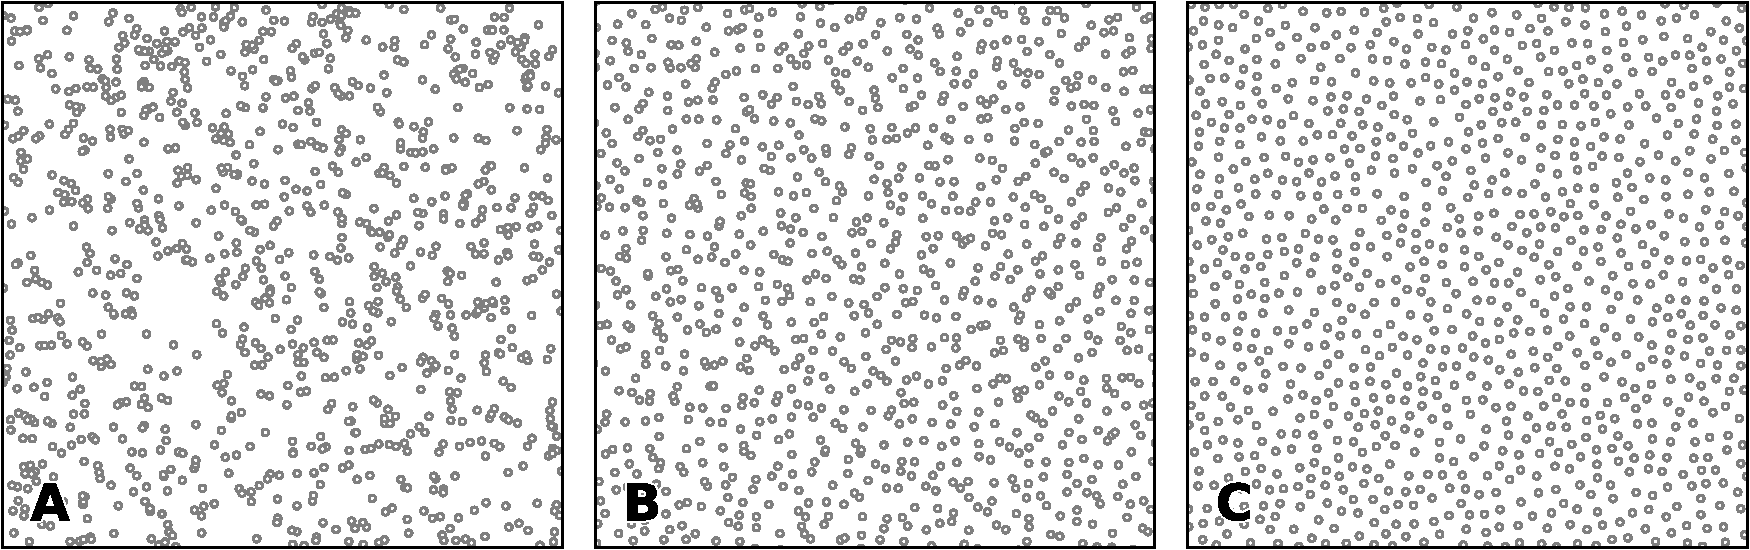
\includegraphics[width=\textwidth]{figure-blue-noise.pdf}
  \caption{\textbf{Spatial distributions.}
    \textbf{\textsf{A.}} Uniform sampling (n=1000) corresponding to white noise.
    \textbf{\textsf{B.}} Regular grid (n=32$\times$32) + jitter (2.5\%).
    \textbf{\textsf{C.}} Poisson disc sampling (n=988) corresponding to blue noise.}
  \label{fig:sampling}
\end{figure}
%%
There exists several methods \citep{Lagae:2008} to obtain blue noise sampling that have been originally designed for computer graphics (e.g. Poisson disk sampling, dart throwing, relaxation, tiling, etc.). Among these methods, the fast Poisson disk sampling in arbitrary dimensions \citep{Bridson:2007} is among the fastest ($\mathcal{O}(n)$) and easiest to use. This is the one we retained for the placement of neurons over the normalized region $[0,1]\times[0,1]$. Such Poisson disk sampling guarantees that samples are no closer to each other than a specified minimum radius. This initial placement is further refined by applying a LLoyd relaxation \citep{Lloyd:1982} scheme for 10 iterations, achieving a quasi centroidal Voronoi tesselation.


%The SOM space is usually defined as a two-dimensional manifold where nodes are arranged in a regular lattice (rectangular or hexagonal). Here, we follow a  different approach and, instead of the regular lattice, we place the neurons randomly by sampling a specific spectral distribution. More specifically, we assign neurons positions by drawing samples from a blue noise distribution. \citep{Zhou:2012}. have shown that the spectral distribution property of noise patterns is often described in terms of the Fourier spectrum color. For instance, white noise corresponds to a flat spectrum with signal's energy equally distributed to all frequency bands while blue  noise has weak low-frequency energy and strong high-frequency energy. An interesting property of the blue noise distribution is that  the resulting positions of neurons drawn are evenly spread without any apparent structure (see figure~\ref{fig:sampling} for a comparison of spatial distributions).
%%
%\begin{figure}[htbp]
%  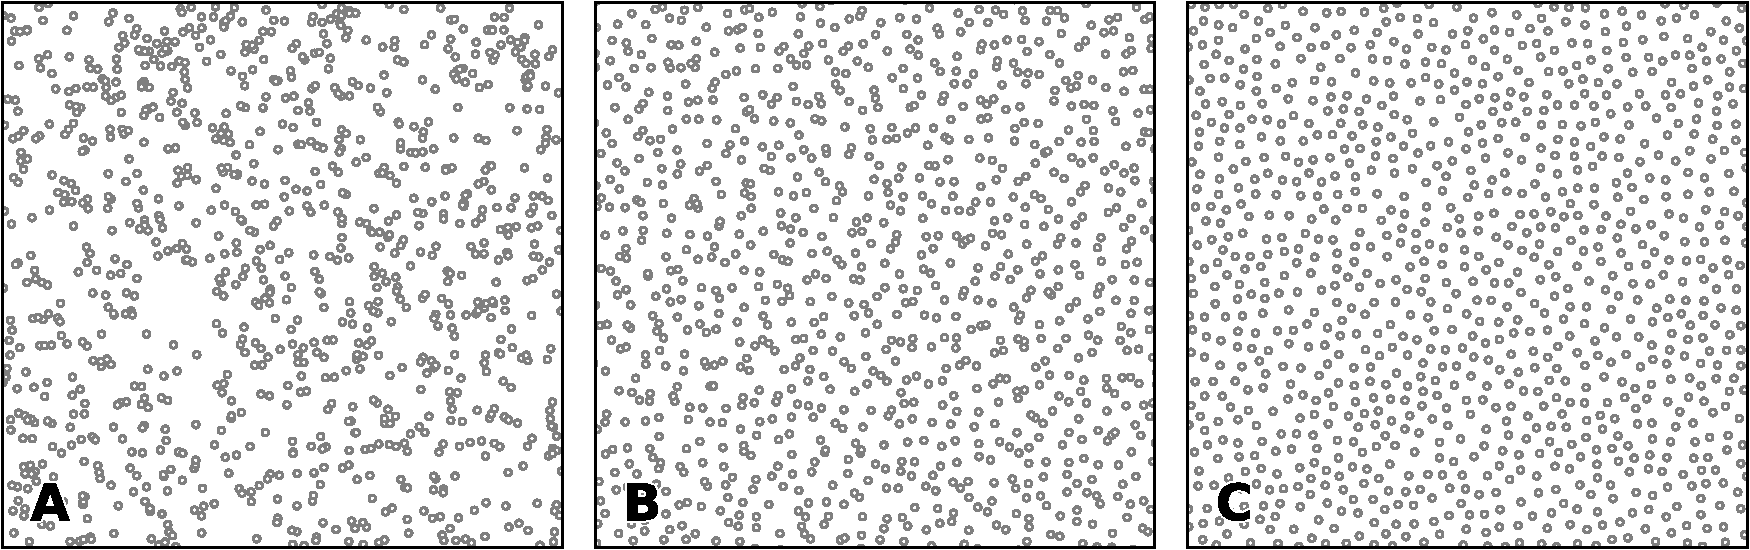
\includegraphics[width=\textwidth]{figures/blue-noise.pdf}
%  \caption{\textbf{Spatial distributions.}
%    \textbf{\textsf{A.}} Uniform sampling (n=1000) corresponding to white noise.
%    \textbf{\textsf{B.}} Regular grid (n=32$\times$32) + jitter (2.5\%).
%    \textbf{\textsf{C.}} Poisson disc sampling (n=988) corresponding to blue noise.}
%  \label{fig:sampling}
%\end{figure}
%%

%Blue noise distributions have been used in the field of computer graphics for many years and there are manych different techniques for computing them: Poisson disk sampling, dart throwing, relaxation, tiling, and other applications (see \citep{Lagae:2008} for a review). One of the fastest and easiest to implement method for generating blue noise samples is the  fast Poisson disk sampling. This method, introduced by \citet{Bridson:2007}, can be used on arbitrary dimensions in linear time ($\mathcal{O}(n)$). In this work, we propose to use this method for placing neurons over a normalized  region of $[0,1]\times[0,1]$. Such Poisson disk sampling guarantees that samples are no closer to each other than a specified minimum radius. This initial placement is further refined by applying a Lloyd relaxation~\cite{Lloyd:1982} scheme for $10$ iterations to achieve a quasi centroidal Voronoi tesselation.

\subsection{Topology}
\label{sec:topo}

Considering a set of $n$ points $P = \{P_i\}_{i \in [1,n]}$ on a finite region,
we first compute the Euclidean distance matrix $E$, where $e_{ij} = \lVert P_i - P_j \rVert$ 
and we subsequently define a connectivity matrix $G^{p}$
%= \{G^{p}_{ij}\}_{i,j \in [1,n]}$ \gid{$G^{p} = g^{p}_{ij},\, \text{where } i,j \in [1,n]$}
such that only the $p$ closest points
are connected. More precisely, if $P_j$ is among the $p$ closest neighbours of
$P_i$ then $g^p_{ij} = 1$ else we have $g^p_{ij} = 0$.
From this connectivity
matrix representing a graph, we compute the length of the shortest path between
each pair of nodes and stored them into a distance matrix $D^p$. Note that
lengths are measured in the number of nodes between two nodes such that two
nearby points (relatively to the Euclidean distance) may have a corresponding
long graph distance as illustrated in figure \ref{fig:topology}. This matrix
distance is then normalized by dividing it by the maximum distance between two
nodes such that the maximum distance in the matrix is 1. In the singular case
when two nodes cannot be connected through the graph, we recompute a spatial
distribution until all nodes can be connected.
%%
\begin{figure}
  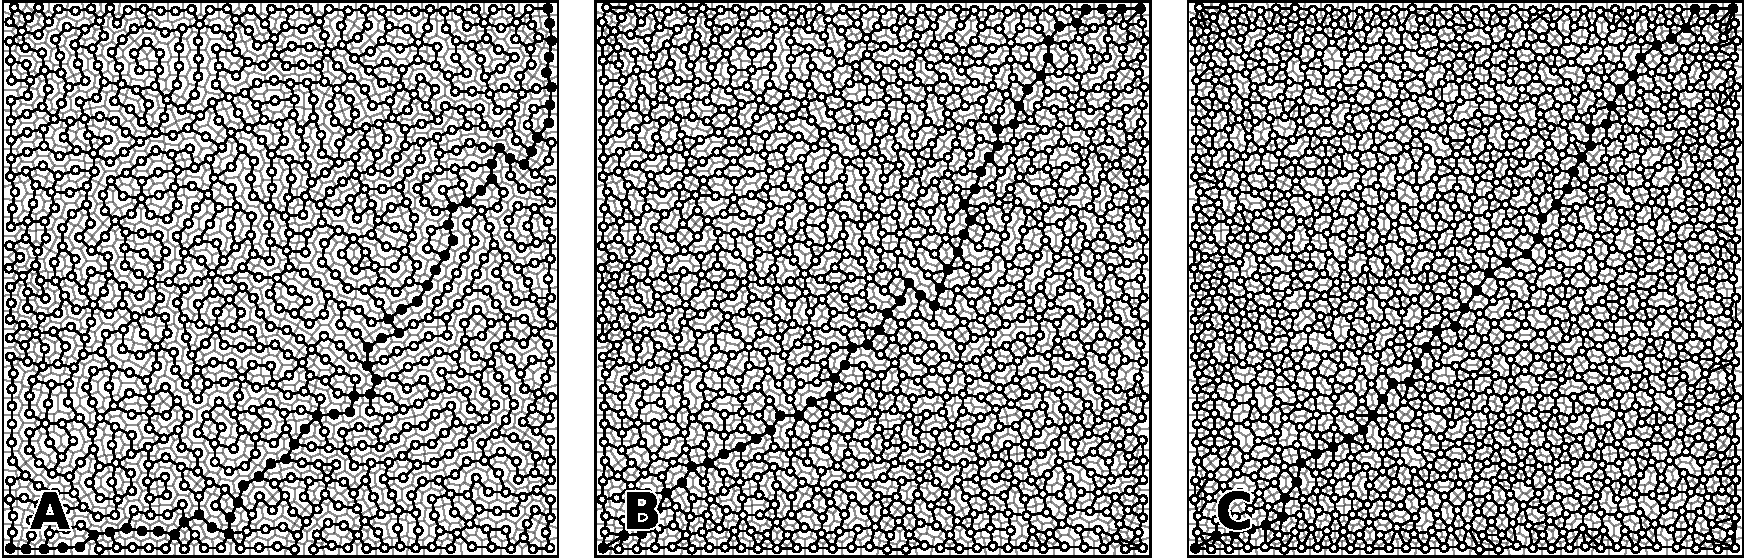
\includegraphics[width=\columnwidth]{figure-distances.pdf}
  \caption{\textbf{Influence of the number of neighbours on the graph
    distance.} The same initial set of 1003 neurons has been equiped with
    2-nearest neighbors, 3 nearest neighbors and 4-nearest neighbors induced
    topology (panels \textbf{A}, \textbf{B} and \textbf{C} respectively). A
    sample path from the the lower-left neuron to the upper-right neuron has
    been highlighted with a thick line (with respective lengths of 59, 50 and
    46 nodes).}
  \label{fig:topology}
\end{figure}

%Consider a set $P$ of $n$ points on a finite region of $[0, 1] \times [0, 1]$. The steps we follow to determine the topology of the SOM are: First, we compute the Euclidean distance matrix ${\bf E} \in \mathbb{R}^{n\times n}$, where $e_{ij} = \lVert p_i - p_j \rVert$ and $i, j=1, \ldots, n$. Subsequently  we define a connectivity matrix ${\bf G}_m$ with elements $g_{ij} = 1$ if $p_j$ belongs to the $m$ closest points to $p_i$ and $g_{ij} = 0$ otherwise. This definition implies that the matrix ${\bf G}_m$ carries information about connected neurons within a predetermined vicinity. Once we compute matrix ${\bf G_m}$, which essentially represents a graph, we compute the shortest path between each pair of nodes on the graph and we store them into a new matrix called ${\bf D}_m$. Note that lengths are measured in number of nodes (hops) required to reach two nodes such that the two corresponding Euclidean points (represented by the nodes) may have a graph distance as illustrated in figure \ref{fig:topology}.  \gid{This matrix distance is then normalized by dividing it by the maximum distance between two nodes. NOT VERY CLEAR}. In the degenerative case where two nodes are not connected on the graph, we resample from a spatial distribution until all nodes have degree greater than one (are connected at least with one other node \gid{IS THIS CORRECT?}).
%%
%\begin{figure}
%  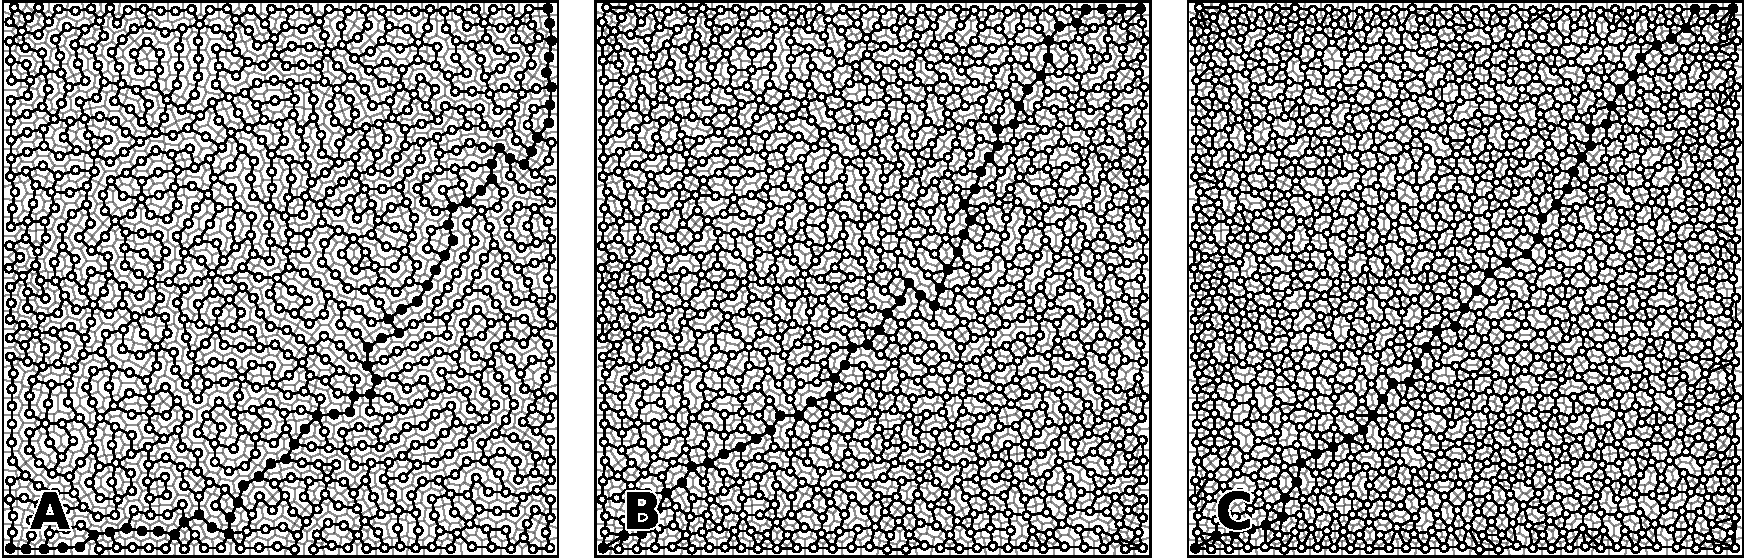
\includegraphics[width=\columnwidth]{figures/distances.pdf}
%\caption{\textbf{Influence of the number of neighbours on the graph distance.} The same initial set of 1003 neurons has been equipped with 2-nearest neighbors, 3 nearest neighbors and 4-nearest neighbors induced topology (panels \textbf{A}, \textbf{B} and \textbf{C} respectively). A sample path from the the lower-left neuron to the upper-right neuron has been highlighted with a thick line (with respective lengths of 59, 50 and 46 nodes).}
%  \label{fig:topology}
%\end{figure}


\subsection{Learning}

The learning process is an iterative process between time $t=0$ and time $t=t_f \in \mathbb{N}^+$ where vectors $\mathbf{v} \in \Omega$ are sequentially presented to the map. For each presented vector $\mathbf{v}$ at time $t$, a winner $s \in \mathcal{N}$ is determined according to equation (\ref{eq:psi}). All codes $\mathbf{w}_{i}$ from the code book are shifted towards $\mathbf{v}$ according to
\begin{equation}
  \Delta\mathbf{w}_{i} = \varepsilon(t)~h_\sigma(t,i,s)~(\mathbf{v} -
  \mathbf{w}_i)
  \label{eq:som-learning}
\end{equation}
with $h_\sigma(t,i,j)$ being a neighborhood function of the form
\begin{equation}
  h_\sigma(t,i,j) = e^{- \frac{{d^p_{ij}}^2}{\sigma(t)^2}}
  \label{eq:som-neighborhood}
\end{equation}
where $\varepsilon(t) \in \mathbb{R}$ is the learning rate and $\sigma(t) \in \mathbb{R}$
is the width of the neighborhood defined as
\begin{equation}
  \sigma(t) =
  \sigma_i\left(\frac{\sigma_f}{\sigma_i}\right)^{t/t_f}, \text{ with } \varepsilon(t) =
  \varepsilon_i\left(\frac{\varepsilon_f}{\varepsilon_i}\right)^{t/t_f},
\end{equation}
while $\sigma_i$ and $\sigma_f$ are respectively the initial and final neighborhood width and $\varepsilon_i$ and $\varepsilon_f$ are respectively the initial and final learning rate. We usually have $\sigma_f \ll \sigma_i$ and $\varepsilon_f \ll \varepsilon_i$.

%The learning algorithm we propose in this work relies on the standard SOM algorithm~\cite{Kohonen:1982}. Once we have define the topology of the map following the steps we described in paragraph~\ref{sec:topo}, we can start the learning process. Learning is iterative and starts at a time $t_0=0$ and runs until some predetermined final time step, $t_f \in \mathbb{N}^+$, has been reached. At every iteration input vectors $\mathbf{v} \in \Omega$ are sequentially given to the map with respect to the probability density function $f$ \gid{Where is defined?}. For each vector $\mathbf{v}$ at time $t$, a winner neuron with index  $s \in \mathcal{N}$ is determined according to equation (\ref{eq:psi}). This means that at time $t$ neuron $s$ is closer to the input vector ${\bf v}$, in the sense of Euclidean distance, than any other neuron. Once the winner neuron has been identified all codes $\mathbf{w}_{i}$ from the current code book are shifted towards $\mathbf{v}$ according to
%\begin{align}
%\label{eq:som-learning}
%    \Delta\mathbf{w}_{i} &= \varepsilon(t)~h(t,i,s;\sigma)~(\mathbf{v} - \mathbf{w}_i), 
%\end{align}
%where $s$ is the index of the winner neuron, $i$ is the index of code words in the code book and $t$ is the current time step. $h_\sigma(t,i,j;\sigma)$ is a neighborhood function of the form
%\begin{equation}
%  h(t,i,j; \sigma) = \exp\Big(-\frac{{d_{ij}}^2}{\sigma(t)^2}\Big)
%  \label{eq:som-neighborhood}
%\end{equation}
%where $\varepsilon: \mathbb{R} \rightarrow \mathbb{R}$ is the learning rate time-dependent function given by $\varepsilon(t) = \varepsilon_i\left(\frac{\varepsilon_f}{\varepsilon_i}\right)^{t/t_f}$, where $\varepsilon_i$ and $\varepsilon_f$ are the initial and final learning rates, respectively. $\sigma: \mathbb{R} \rightarrow \mathbb{R}$ is determines the width of the  neighborhood function~\eqref{eq:som-neighborhood} and it is reads $\sigma(t) = \sigma_i\left(\frac{\sigma_f}{\sigma_i}\right)^{t/t_f}$, where $\sigma_i$ and $\sigma_f$ are the initial and final neighborhood widths, respectively. We usually assume $\sigma_f \ll \sigma_i$ and  $\varepsilon_f \ll \varepsilon_i$. The entire learning procedure is summarized by Algorithm~\ref{algo:vsom}. 

%% %%
\begin{algorithm}[!htpb]
	\begin{algorithmic}
    	\Require $\mathcal{S}$, $\mathcal{N}$, $t_f$, $dt$, $\varepsilon_i$, $\varepsilon_f$, $\sigma_i$, $\sigma_f$
        \Ensure ${\bf W}$
        \If {\text{Blue noise is True}}
        	\State Compute blue noise distribution $\mathcal{B}$
        	\State Compute $e_{ij} = || p_i - p_j ||$		\Comment{Euclidean pair distances matrix}
        	\State Construct matrix ${\bf G}_m$			\Comment{Connectivity matrix}
        	\State Compute matrix ${\bf D}_m$			\Comment{Shortest paths between nodes}
        	\State Place neurons positions on points sampled from $\mathcal{B}$
        \Else
        	\State Discretize grid $[0, 1]\times[0, 1]$ and place neurons on its nodes
        \EndIf
        
        \State $w_s \gets \varnothing$, ${\bf W} \sim \mathcal{U}(0, 1)$	\Comment{Initialize winner unit and code book}
                 
        \For{$t \gets 0, \ldots, t_f$}
        	\State ${\bf v} \gets \bf{s}_t $	\Comment{${\bf s}_t \in \mathcal{S}$}
        	\State $s \gets argmin_{i \in \mathcal{N}} (\lVert \mathbf{v} - \mathbf{w}_i \rVert)$
        	\State $\varepsilon(t) = \varepsilon_i\left(\frac{\varepsilon_f}{\varepsilon_i}\right)^{t/t_f}$
        	\State $\sigma(t) = \sigma_i\left(\frac{\sigma_f}{\sigma_i}\right)^{t/t_f}$
        	\State $h(t,i,j; \sigma) = \exp\Big(-\frac{{d_{ij}}^2}{\sigma(t)^2}\Big)$
        	\State ${\bf w}_i^{\text{new}} = {\bf w}_i^{\text{old}} + \varepsilon(t) \odot h(t,i,s;\sigma) \odot (\mathbf{v} - \mathbf{w}_i^{\text{old}})$
        \EndFor
	\end{algorithmic}
\caption{Voronoi Self-organizing Map (vSOM). $\mathcal{N}$ is neurons index set,
$\mathcal{I}$ is the input dataset, $t_f$ is the simulation time (or the number of input samples).
$\varepsilon_i$ and $\varepsilon_f$ are the initial and final learning rates,
respectively. $\sigma_i$ and $\sigma_f$ are the initial and final neighborhood
widths. $\odot$ is the Hadamard product.}
\label{algo:vsom}
\end{algorithm}
%%


\subsection{Analysis Tools}
In order to analyze and compare the results of RSOM and SOM, we used a spectral method and persistence diagram analysis on the respective codebooks. These analysis tools are detailed below but roughly, the spectral method allows to estimate the distributions of eigenvalues in the activity of the maps while the persistence diagram allows to check for discrepancies between the topology of the input space and the topology of the map.

% To analyze the results of both the Kohonen SOM and VSOM algorithms and to make any comparison between the two algorithms we use a spectral method and persistence diagram on codebooks. The spectral method estimates the distributions of eigenvalues of the activity of neurons. The persistence diagram is a topological-geometrical  approach, more precisely is a tool coming from the field of topological data analysis (TDA). TDA provides the tools to investigate the topology of the maps and the input space and spot differences between the topology of the input space and the neural space of the SOM algorithms (Kohonen and VSOM). 

%\subsubsection{Topological Data Analysis}
\label{sec:tda}

Topological Data Analysis (TDA) \citep{Carlsson:2009} provides methods and tools to study topological structures of data sets such as point cloud and is useful when geometrical or topological information is not apparent within a data set. Furthermore, TDA tools are insensitive to dimension reduction and noise which make them well suited to analyze high-dimensional self-organized maps and their corresponding input data sets. In this work, we use the notion of persistent barcodes and diagrams \citep{Edelsbrunner:2008} to spot any differences between the topology of the input and neural spaces. Furthermore, we can apply some metrics from TDA such as the Bottleneck distance and measure how close two persistent diagrams are.
% qualify the quality of the representations of a map.
Since the exact manifold (or distribution) of the input space is not known in general and the SOM algorithms only approximate it, we simplify these manifolds by retaining their original topological structure.
Here we approach the manifolds of input and neural spaces using the Alpha complex. Before diving into more details regarding TDA, we provide here a few definitions and some notation. A $k$-simplex $\sigma$ is the convex hull of $k+1$ affinely independent points (for instance a $0$-simplex is a point, a $1$-simplex is an edge, a $2$-simplex is a triangle, etc). A simplicial complex with vertex set $\mathcal{V}$ is a set $\mathcal{S}$ of finite subsets of $\mathcal{V}$ such that the elements of $\mathcal{V}$ belong to $\mathcal{S}$ and for any $\sigma \in \mathcal{S}$ any subset $\sigma$ belongs to $\mathcal{S}$. Said differently, a simplicial complex is a space that has been  constructed out of intervals, triangles, and other higher dimensional simplices.

In our analysis we let $\mathcal{S}(\mathcal{M}, \alpha)$ be a Alpha simplicial complex with $\mathcal{M}$ being a point cloud, either the input space or the neural one, and $\alpha$ is the ``persistence'' parameter. More specifically, $\alpha$ is a threshold (or radius as we will see later) that determines if the set $X$ spans a $k$-simplex if and only if $d(x_i, x_j) \leq \alpha$ for all $0 \leq i, j \leq k$. From a practical point of view, we first define a family of thresholds $\alpha$ (or radius) and for each $\alpha$, we center a ball of radius $\alpha$ on each data point and look for possible intersections with other balls. This process is called filtration of simplicial complexes. We start from a small $\alpha$ where there are no intersecting balls (disjoint set of balls) and steadily we increase the size of $\alpha$ up to a point where a single connected blob emerges. As $\alpha$ varies from a low to a large value, holes open and close as different balls start intersecting. Every time an intersection emerges we assign a {\em birth} point $b_i$ and as the $\alpha$ increases and some new intersections of larger simplicies emerge some of the old simplicies die (since they merge with  other smaller simplicies to form larger ones). Then we assign a {\em death} point $d_i$. A pair of a birth and death points $(b_i, d_i)$ is plotted on a Cartesian two-dimensional plane and indicates when a simplicial complex was created and when it died. This two-dimensional diagram is called persistent diagram and the pairs (birth, death) that last longer reflect significant topological properties. The longevity of birth-death pairs is more clear in the persistent barcodes where the lifespan of such a pair is depicted as a straight line.

In other words, for each value of $\alpha$ we obtain new simplicial complexes and thus new topological properties such as  homology are revealed. Homology encodes the number of  points, holes, or voids in a space. For more thorough reading we refer the reader to \citep{Chazal:2017,Ghrist:2008,Zomorodian:2005}. In this work, we used the Gudhi library~\citep{Maria:2014} to compute the Alpha simplicial complexes, the filtrations and the persistent diagrams and barcodes. Therefore, we compute the persistent diagram and persistent barcode of the input space and of the maps and we calculate the Bottleneck distance between the input and SOM and RSOM maps diagrams. The bottleneck distance provides a tool to compare two persistent diagrams in a quantitative way. The Bottleneck distance between two persistent diagrams $\text{dgm}_1$ and $\text{dgm}_2$ as it is described in~\cite{Chazal:2017}
%%
\begin{align}
    \label{eq:bottle}
    d_b(\text{dgm}_1, \text{dgm}_2) &= \inf_{\text{matching }m}\{ \max_{(p, q) \in m} \{||p - q||_{\infty} \} \},
\end{align}
%%
where $p \in \text{dgm}_1 \backslash \Delta$, $q \in \text{dgm}_2 \backslash \Delta$, $\Delta$ is the diagonal of the persistent diagram (the diagonal $\Delta$ represents all the points that they die the very moment they get born, $b = d$). A matching between two  diagrams $\text{dgm}_1$ and $\text{dgm}_2$ is a subset $m \subset \text{dgm}_1 \times \text{dgm}_2$ such that every point in $\text{dgm}_1 \backslash \Delta$ and $\text{dgm}_2 \backslash \Delta$ appears exactly once in $m$. 

% In a similar way the Wasserstein distance is  defined by
% %%
% \begin{align}
%     \label{eq:wasser}
%     W_p(\text{dgm}_1, \text{dgm}_2)^p &= \inf_{\text{matching } m} \{ \sum_{(p, q) \in m}^{} ||p - q||^p_{\infty} \}.
% \end{align}
% %%



\subsection{Simulation Details}

Unless specified otherwise, all the models were parameterized using values given in table \ref{table:parameters}. These values were chosen to be simple and do not really impact the performance of the model. All simulations and figures were produced using the Python scientific stack, namely, SciPy \citep{Jones:2001}, Matplotlib \citep{Hunter:2007}, NumPy \citep{Walt:2011}, Scikit-Learn \citep{Pedregosa:2011}. Analysis were performed using Gudhi \citep{Maria:2014}). 
Sources are available at \href{https://github.com/rougier/VSOM}{github.com/rougier/VSOM}.
%%
\begin{table}[!ht]
  \begin{center}
    \begin{tabular}{ll}
        \textbf{Parameter} & \textbf{Value} \\
        \hline
        Number of epochs      ($t_f$)           & 25000\\
        Learning rate initial ($\varepsilon_i$) & 0.50\\
        Learning rate final   ($\varepsilon_f$) & 0.01\\
        Sigma initial         ($\sigma_i$)      & 0.50\\
        Sigma final           ($\sigma_f$)      & 0.01\\
    \end{tabular}
      \caption{\textbf{Default parameters} Unless specified otherwise, these are
        the parameters used in all the simulations.}
      \label{table:parameters}
  \end{center}
\end{table}

%We conduct all the experiments using the parameters provided by Table~\ref{table:parameters}. In all the experiments the input space is the Cartesian product $[0, 1] \times [0, 1]$ and neurons positions drawn from a blue noise distribution using the fast Poisson disk sampling algorithm~\cite{Bridson:2007} (see paragraph~\ref{sec:spatial_dist} for more details).  The source code of the proposed algorithm is written in the Python programming language (SciPy~\cite{Jones:2001}, Matplotlib~\cite{Hunter:2007} and NumPy~\cite{Walt:2011}, Scikit-Learn~\cite{Pedregosa:2011}, Gudhi~\cite{Maria:2014}). Sources are available at \href{https://github.com/rougier/VSOM}{github.com/rougier/VSOM}.


%% Considering a set of $n$ points $P = \{P_i\}_{i \in [1,n]}$ on a finite domain
%% $D \in \mathbb{R}^2$, the Voronoi tesselation $V(P) = \{V_i\}_{i \in [1,n]}$ of
%% $P$ is defined as:
%% %
%% \begin{equation}
%%   \forall i \in [1,n], V_i = \{x \in D \mid
%%   \lVert x - P_i \rVert \leq \lVert x - P_j \rVert, \forall j \neq i\}
%% \end{equation}
%% %
%% Reciprocally, the (unique) Delaunay triangulation $T(P) = \{T_i\}_{i \in
%%   [1,n]}$ of $P$ is the dual graph of the Voronoi diagram and defined such that
%% no point in $P$ is inside the circumcircle of any triangles in $T(P)$. The
%% centers of the circumcircles are equivalent to the Voronoi diagram, i.e. a
%% partition of $D$ into Voronoi cells. For each of the cell $V_i$, we can compute
%% its centroid $C_i$ which is the center of mass of the cell. A Voronoi
%% tesselation is said to be centroidal when we have $\forall i \in [1,n], C_i =
%% P_i$ (see figure~\ref{fig:CVT}).\\

%% For an arbitrary set of points, there is no guarantee that the corresponding
%% Voronoi tesselation is centroidal but different methods can be used to
%% generate a centroidal tesselation from an arbitrary set of points. One of the
%% most straightforward and iterative methods is the Lloyd relaxation scheme
%% \cite{Lloyd:1982}:
%% \begin{enumerate}
%%   \item The Voronoi diagram of the $n$ points is computed
%%   \item The centroid of each of the $n$ Voronoi cell is computed.
%%   \item Each point is moved to the corresponding centroid of its Voronoi cell
%%   \item The method terminates if criterion is met (see below), else go to 1
%% \end{enumerate}
%% The algorithm finishes when the maximum distance between points and centroids
%% is less than a given threshold as illustrated in figure~\ref{fig:CVT}. It is
%% to be noted that because of numerical imprecisions, there is no guarantee that
%% an arbitrary small threshold can be reached.


%% \begin{figure}[htbp]
%%   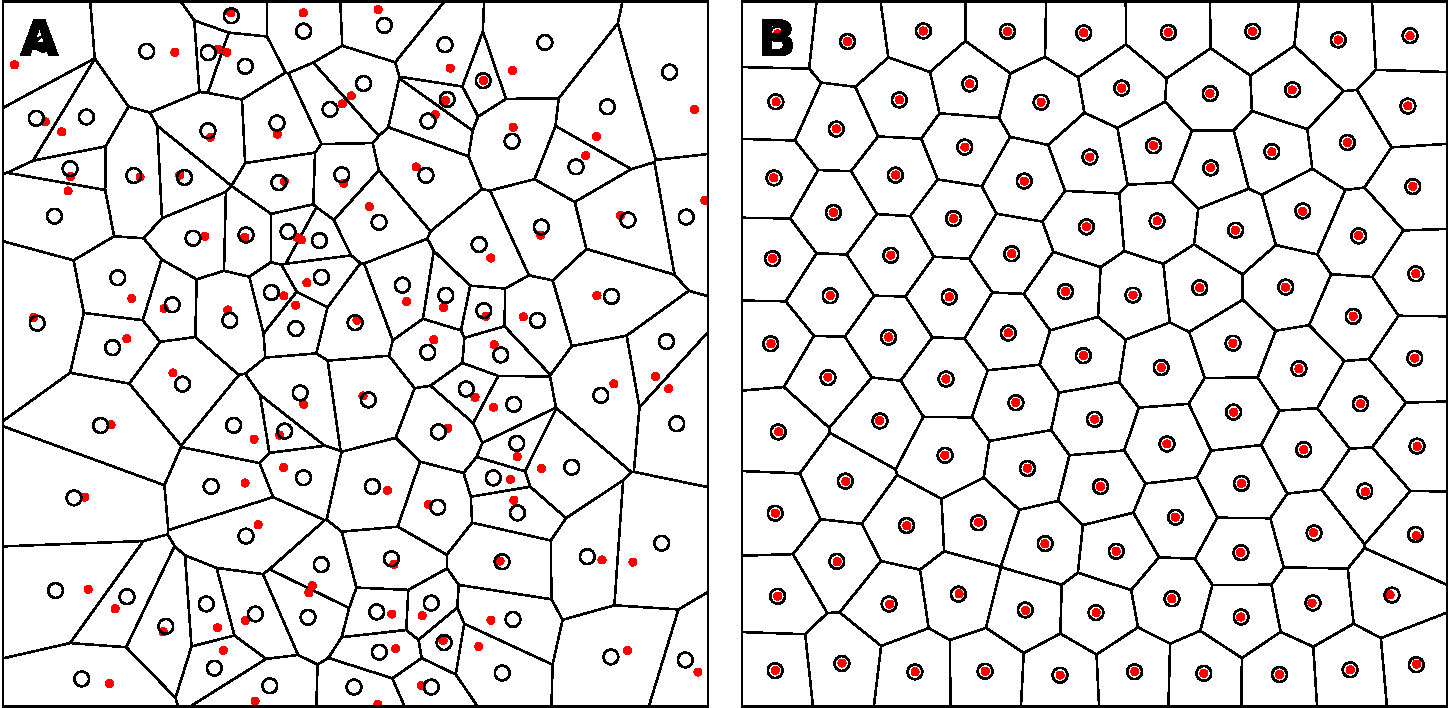
\includegraphics[width=\textwidth]{figures/CVT.pdf}
%%   \caption{\textbf{Centroidal Voronoi Tesselation.}  \textbf{\textsf{A.}}
%%     Voronoi diagram of a uniform distribution (n=100) where red dots represent
%%     the uniform distribution and white circles represent the centroids of each
%%     Voronoi cell. \textbf{\textsf{B.}} Centroidal Voronoi diagram where the
%%     point distribution matches the centroid distribution which constitutes a
%%     blue noise distribution (i.e. {\em a distribution that is roughly uniformly
%%       random with no preferred inter-point directions or distances} according
%%     to the definition of \cite{Ebeida:2014}). This figure has been obtained
%%     from the initial distribution on the left after 50 iterations of the Lloyd
%%     relaxation algorithm. }
%%   \label{fig:CVT}
%% \end{figure}
%

\section{Results}


\subsection{Low-dimensional data}

\subsubsection*{One-dimensional data}

\begin{figure}
  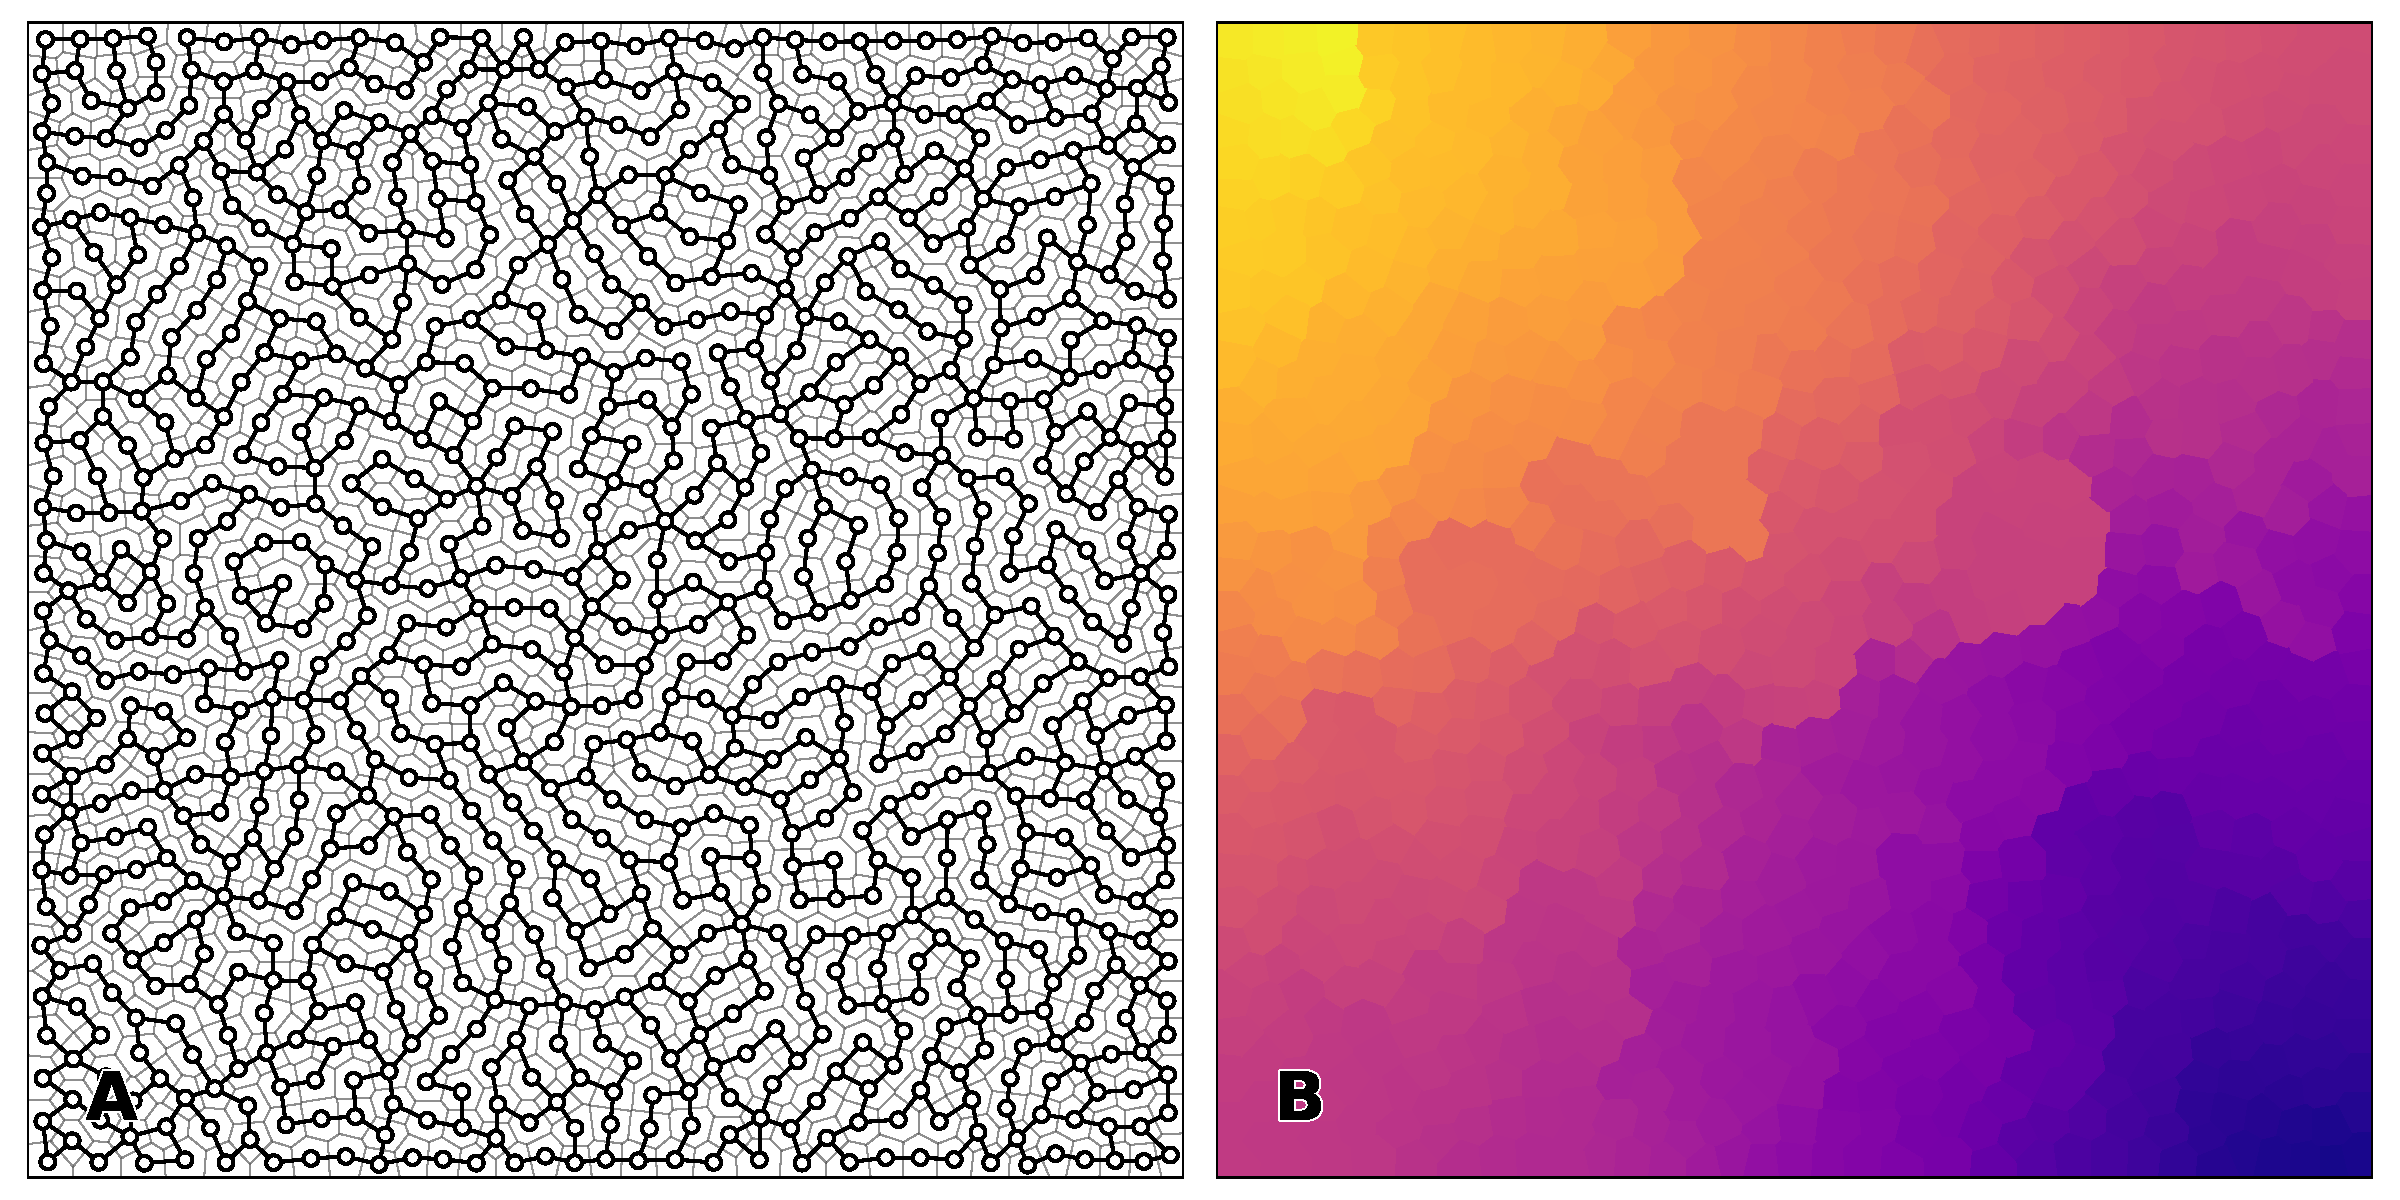
\includegraphics[width=\columnwidth]{figures/vsom-scalar-1.pdf}

  \vspace{2mm}
  
  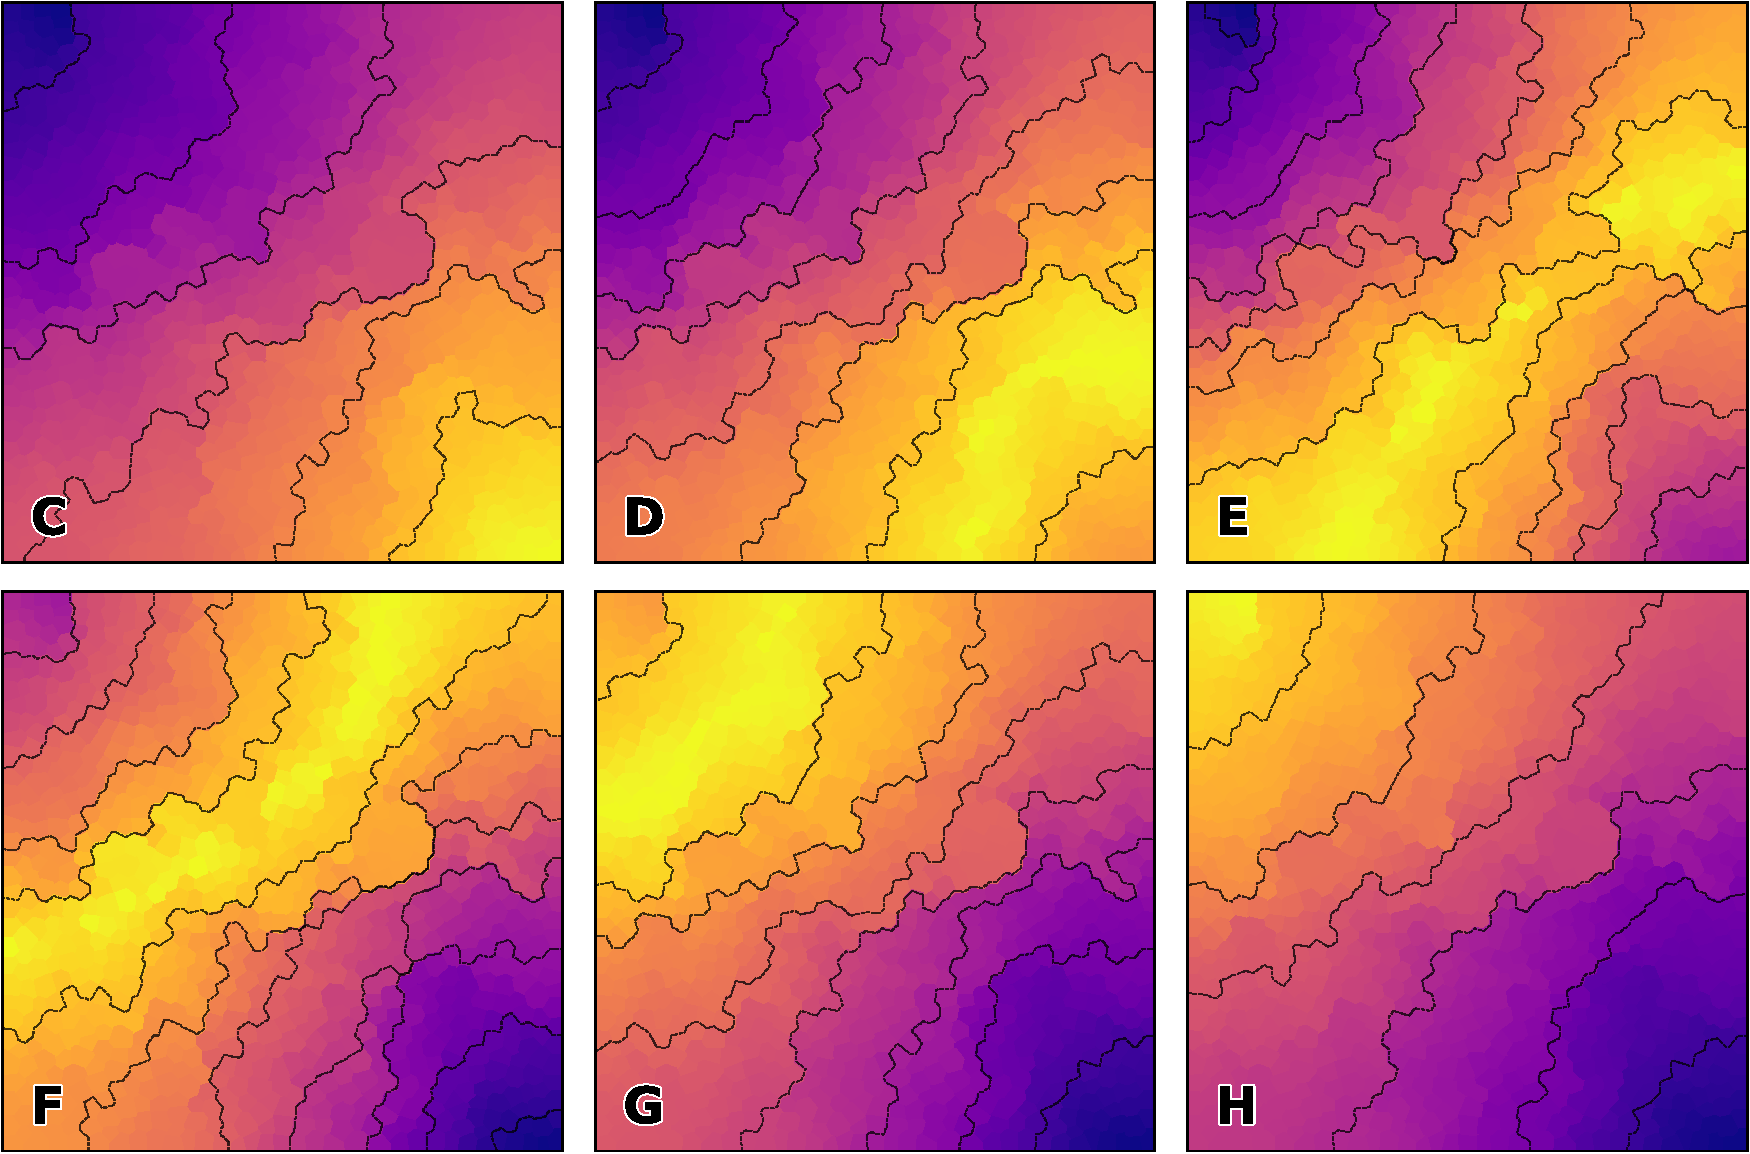
\includegraphics[width=\columnwidth]{figures/vsom-scalar-2.pdf}

  \vspace{2mm}
  
  \includegraphics[width=\columnwidth]{figures/colormap.pdf}
  
  \caption{Voronoidal SOM made of 1003 neurons with a 2-nearest neighbors
    induced topology. Model has been trained for 10,000 epochs on random
    uniform scalars in [0,1]. \textbf{A} Map topology in the neural
    space. \textbf{B} Map prototypes displayed in neural space using Voronoi
    cells (whose color indicates prototype according to colormap). \textbf{C to
      H} Map activity for some random data (\textbf{C}:0.0, \textbf{D}:0.2,
    \textbf{E}: 0.4, \textbf{F}:0.6, \textbf{G}:0.8, \textbf{H}:1.0).}
\end{figure}

\begin{figure}
  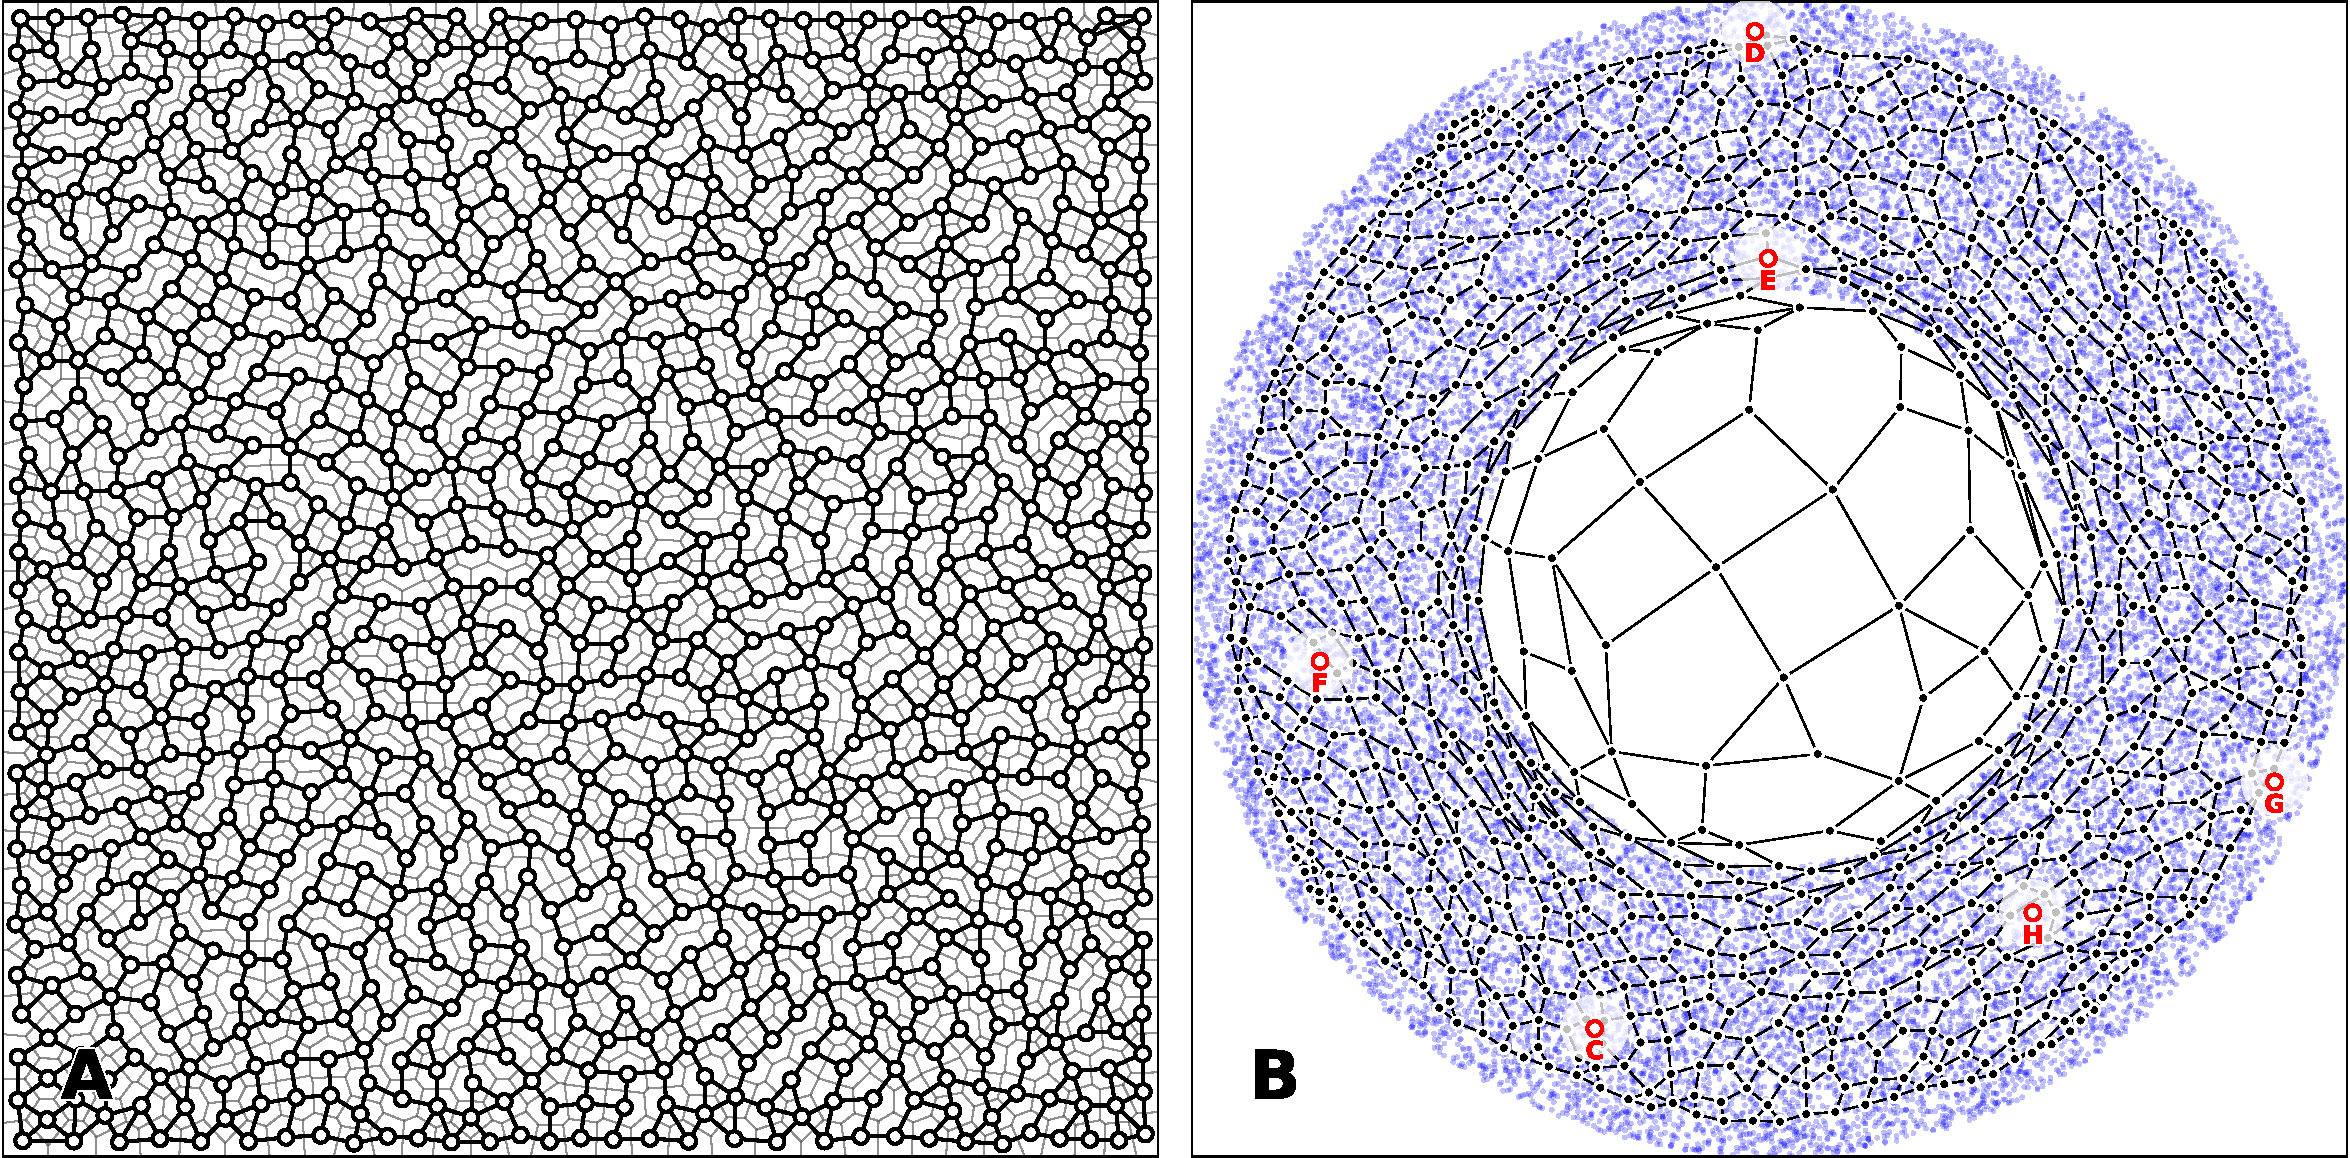
\includegraphics[width=\columnwidth]{figures/vsom-spatial-1.pdf}

  \vspace{2mm}
  
  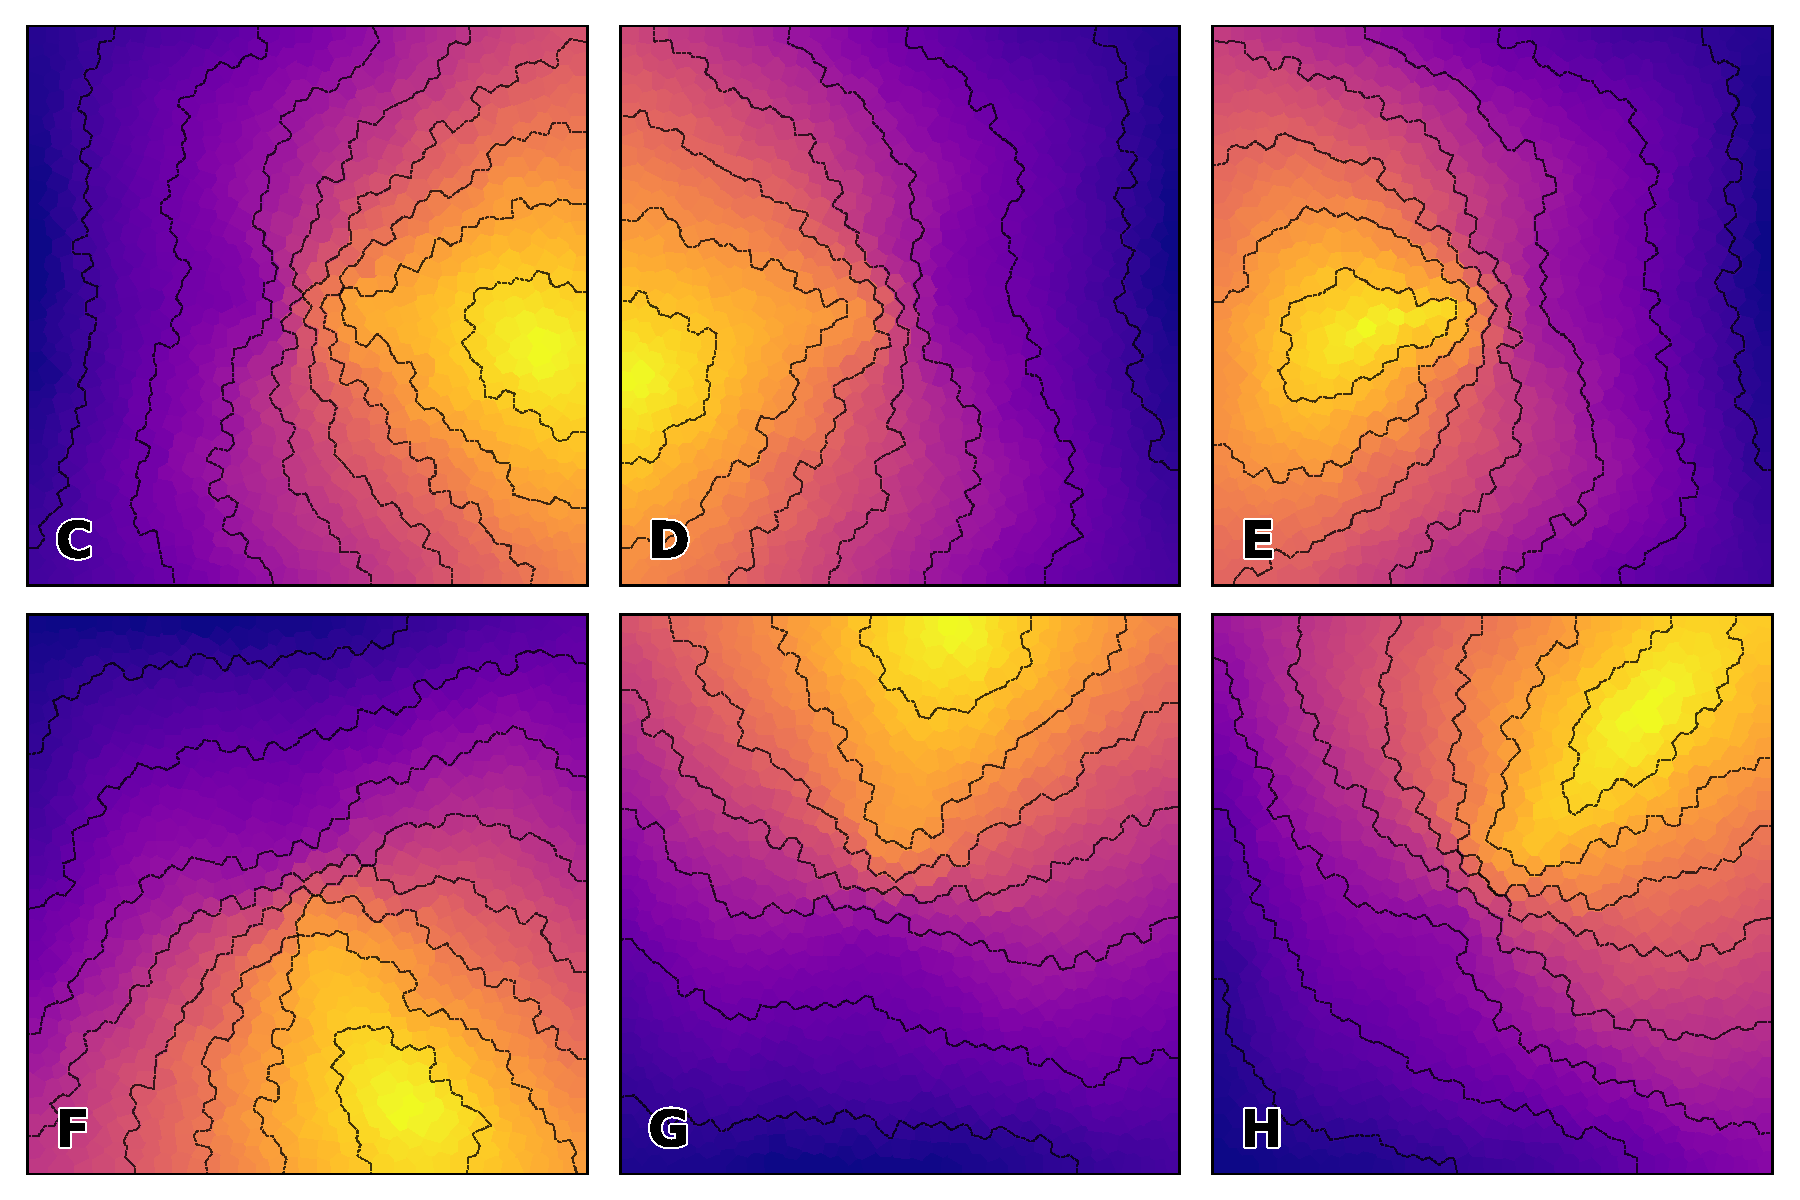
\includegraphics[width=\columnwidth]{figures/vsom-spatial-2.pdf}

  \vspace{2mm}

  \includegraphics[width=\columnwidth]{figures/colormap.pdf}
  \caption{Voronoidal SOM made of 1003 neurons with a 3-nearest neighbors
    induced topology. Model has been trained for 25,000 epochs on random
    samples inside a torus. \textbf{A} Map topology in the neural
    space. \textbf{B} Map prototypes displayed in data space, blue points are
    the actual samples. \textbf{C to H} Map activity for some random data
    (shown on subplot \textbf{B}).}
\end{figure}

\begin{figure}
  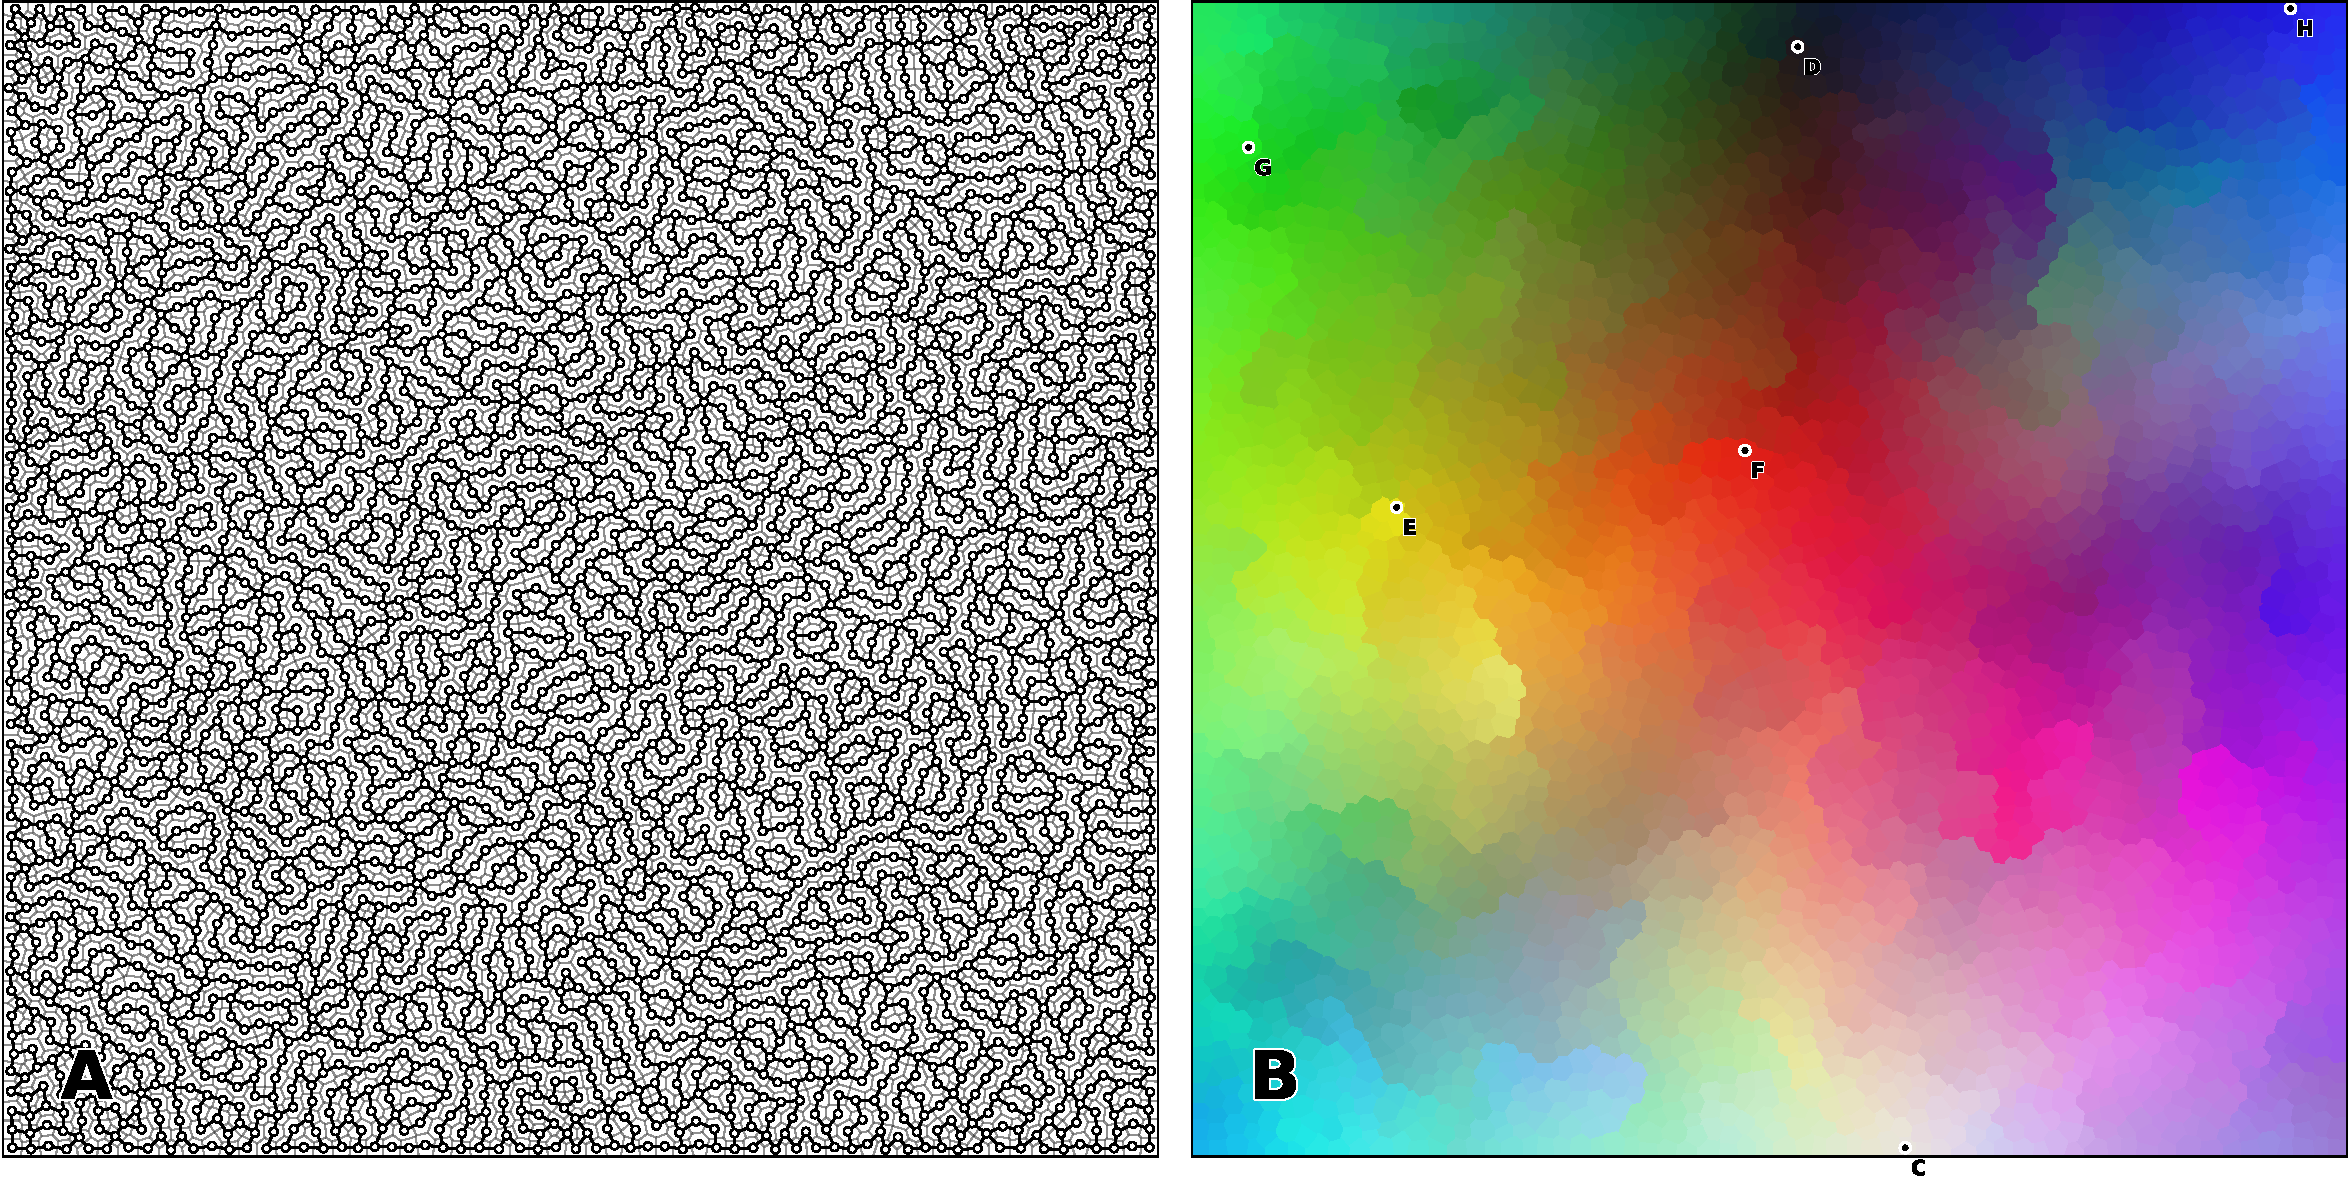
\includegraphics[width=\columnwidth]{figures/vsom-colors-1.pdf}

  \vspace{2mm}
  
  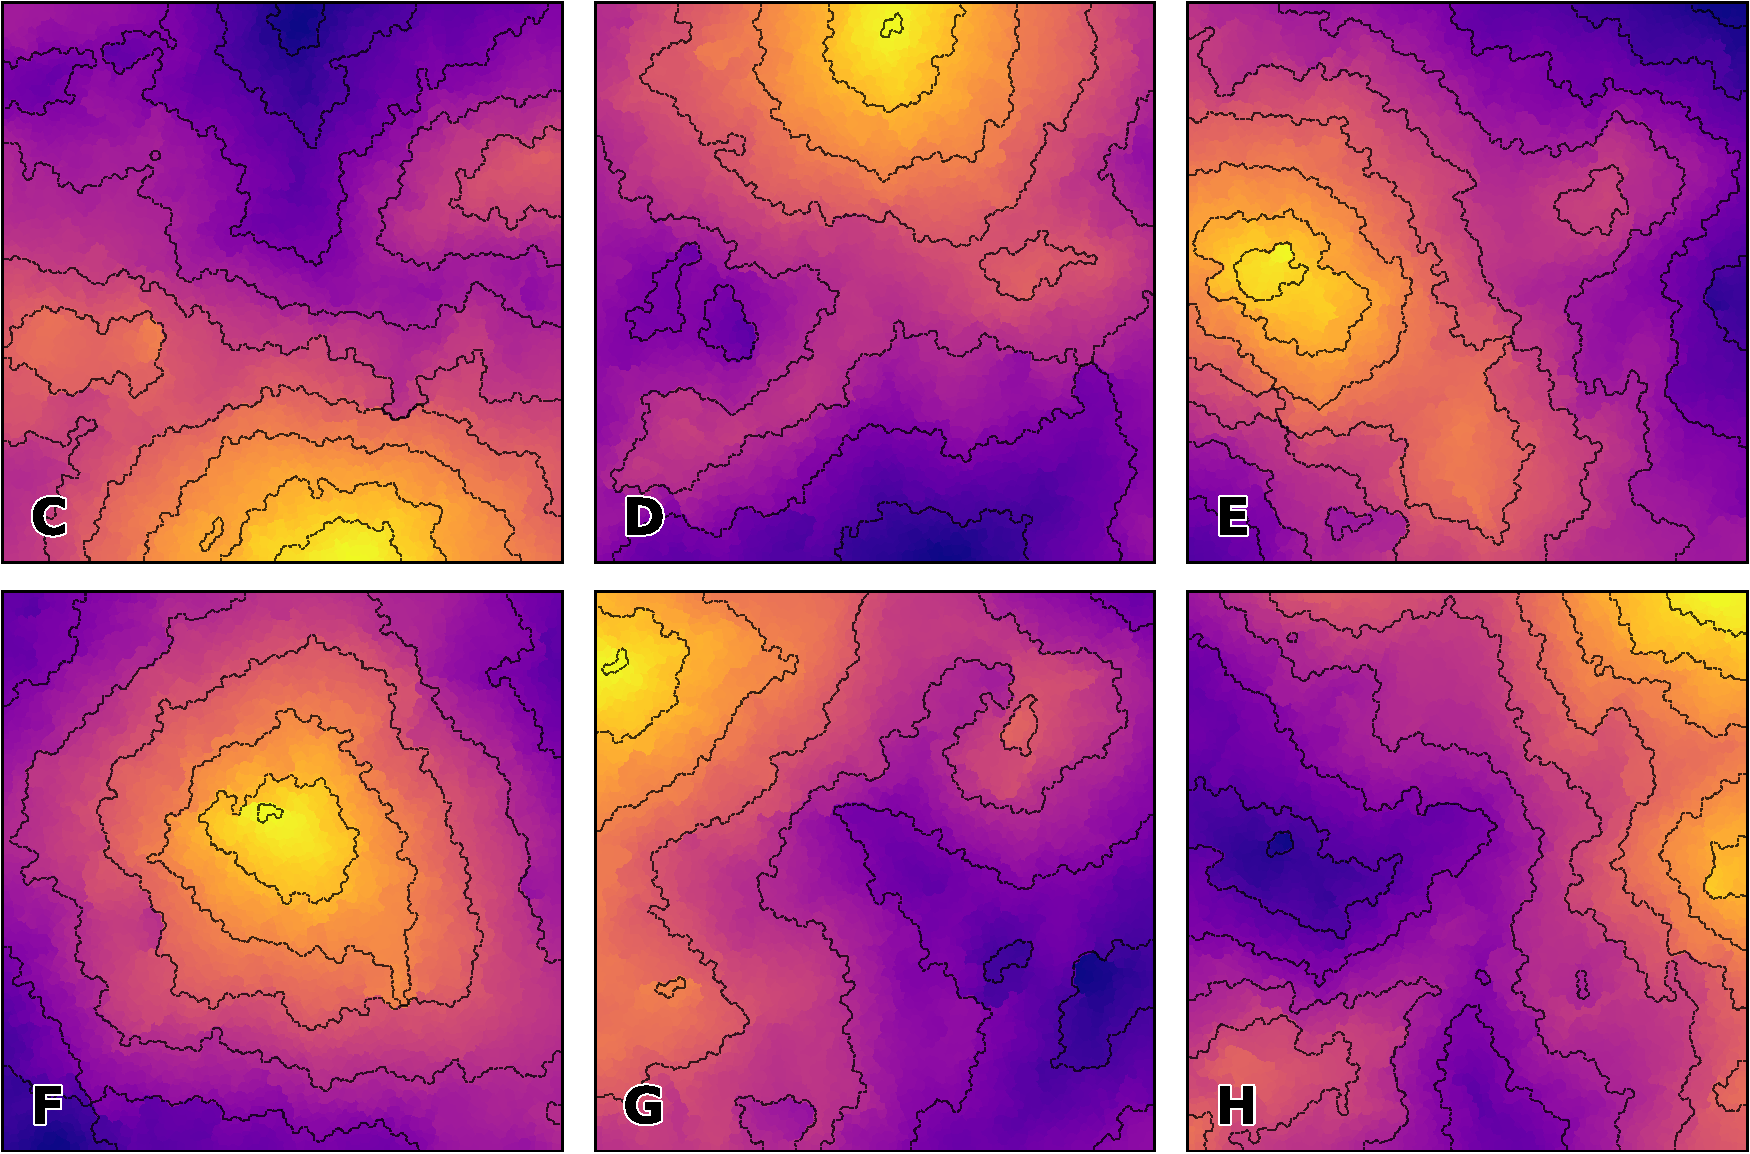
\includegraphics[width=\columnwidth]{figures/vsom-colors-2.pdf}

  \vspace{2mm}

  \includegraphics[width=\columnwidth]{figures/colormap.pdf}

  \caption{}
\end{figure}

\subsection{High-dimensional data}






\begin{figure}
  \setlength{\fboxsep}{0pt}%
  \setlength{\fboxrule}{.25pt}%

  \fbox{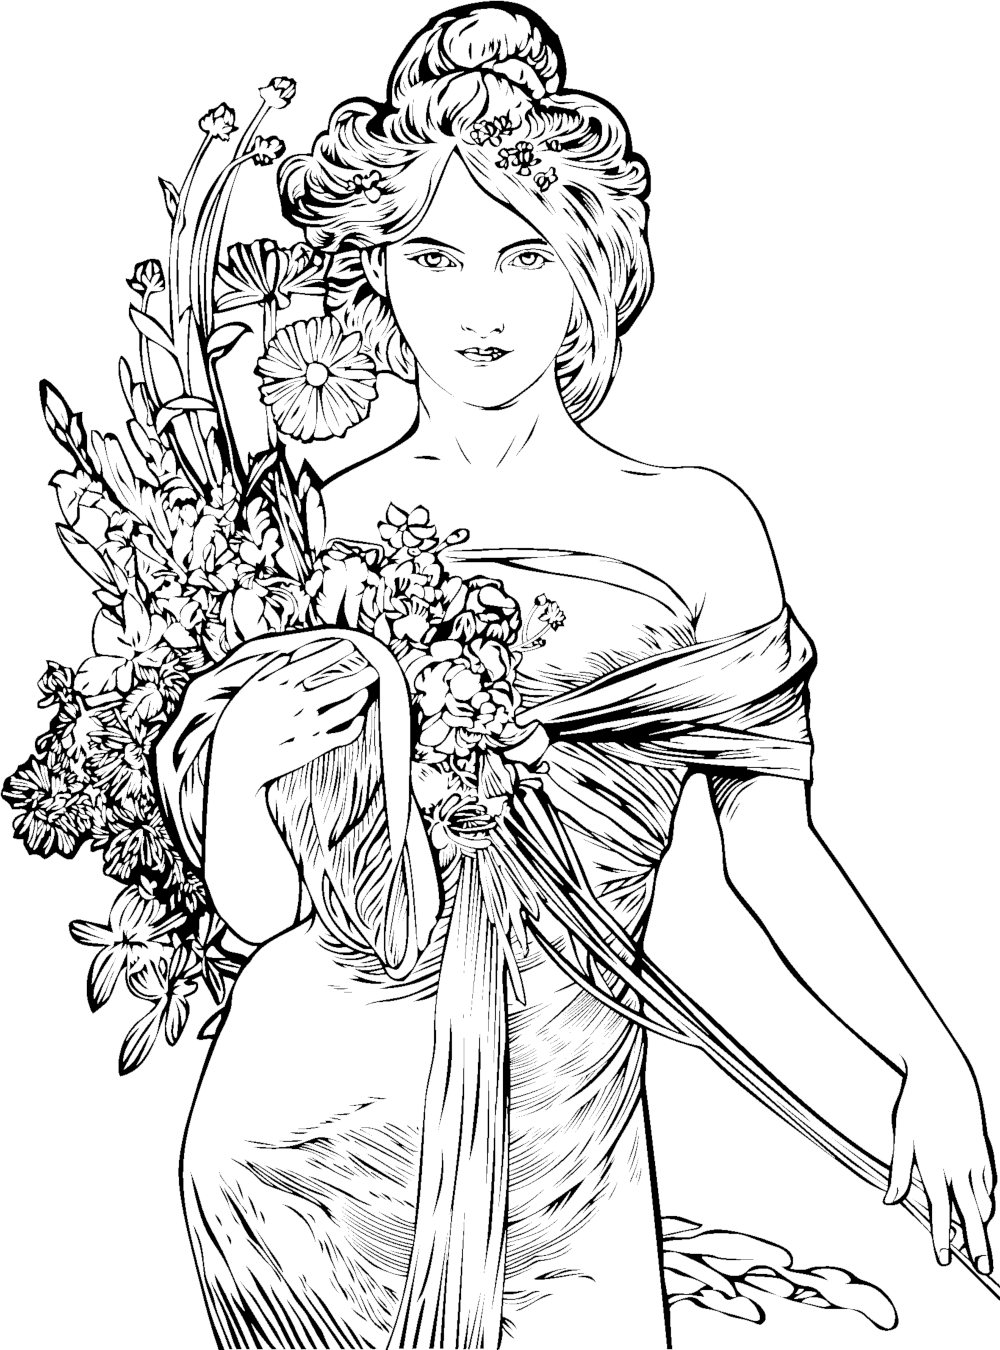
\includegraphics[height=5.1cm]{figures/mucha.png}}
        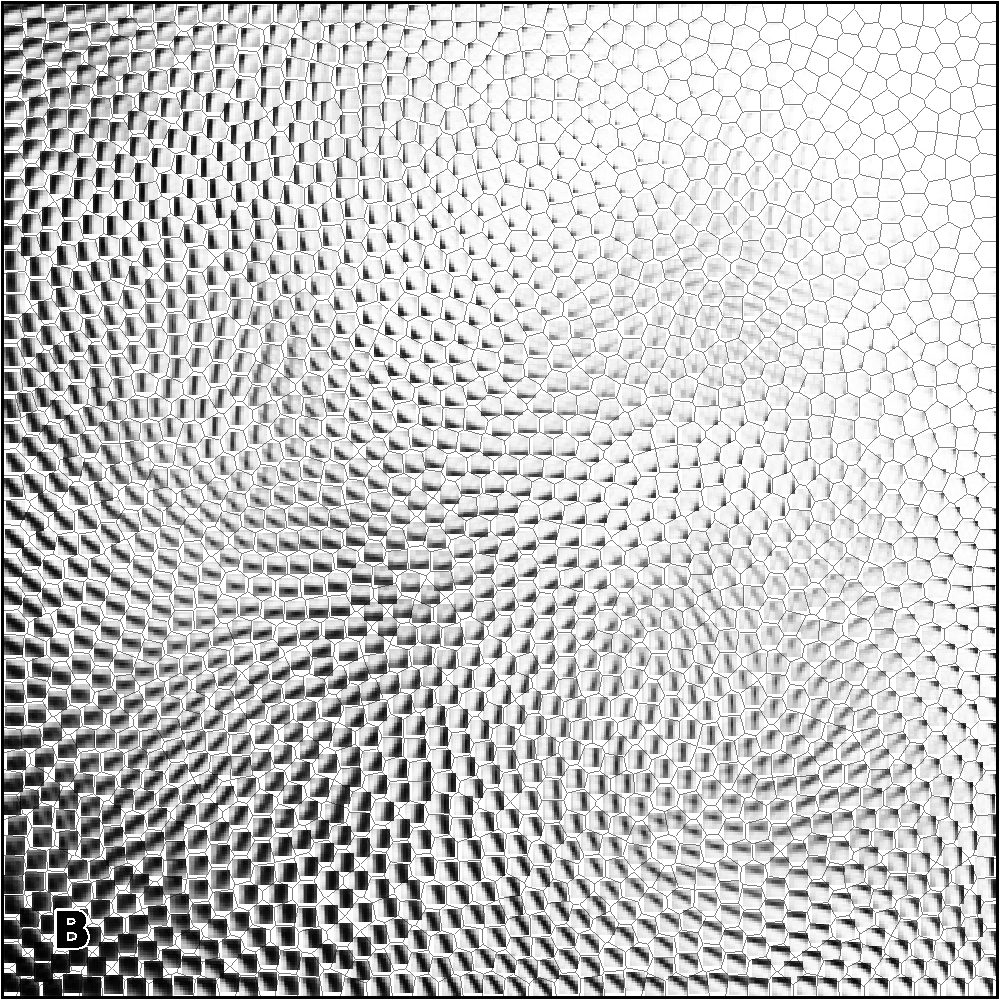
\includegraphics[height=5.1cm]{figures/vsom-image.pdf}
  \fbox{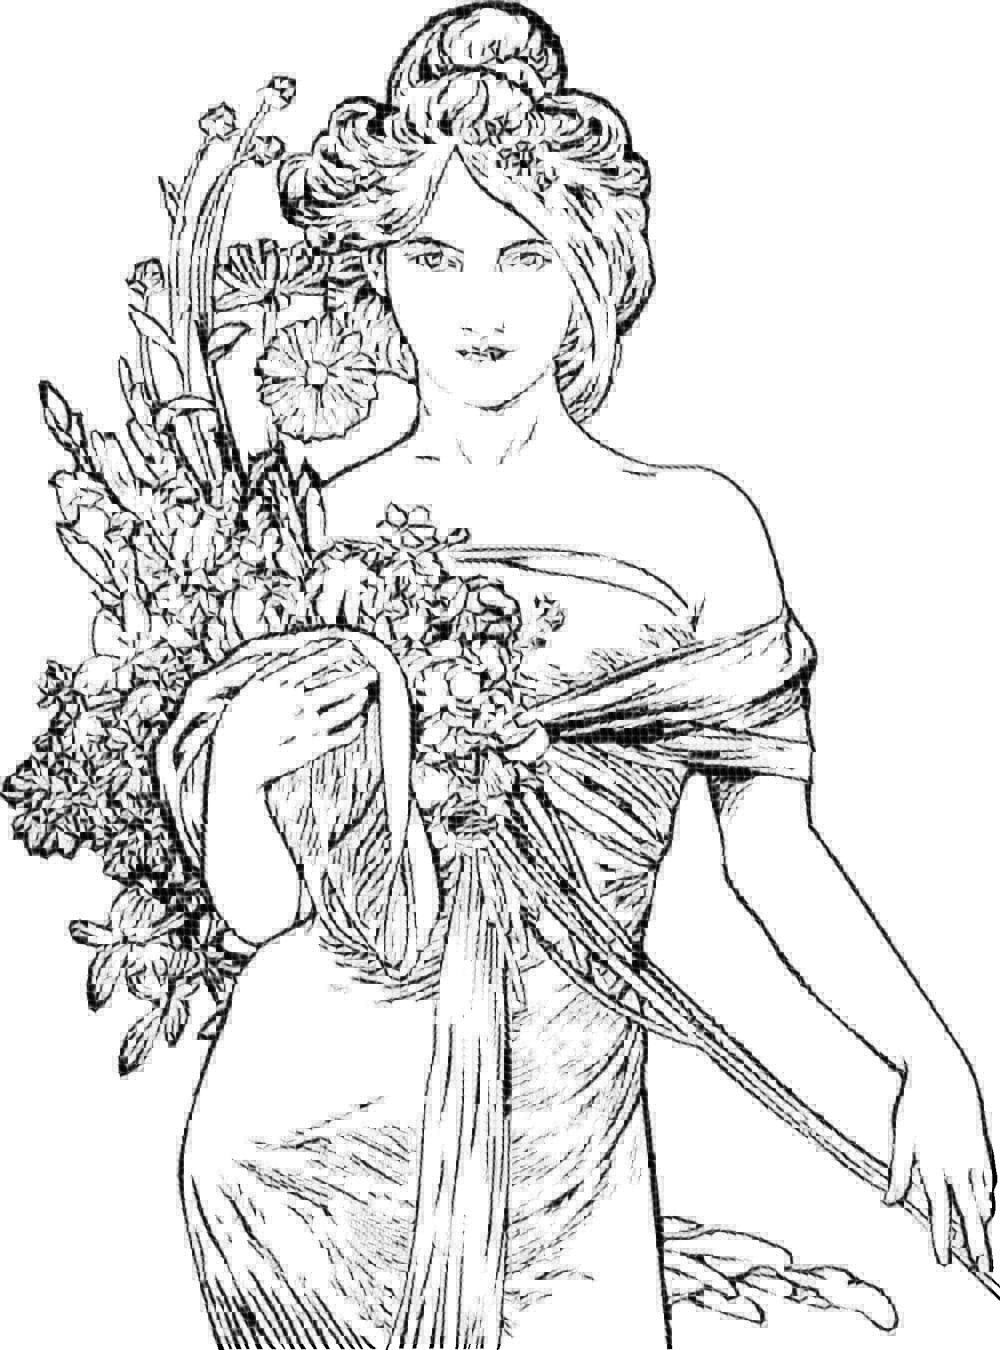
\includegraphics[height=5.1cm]{figures/mucha-vsom.png}}

%  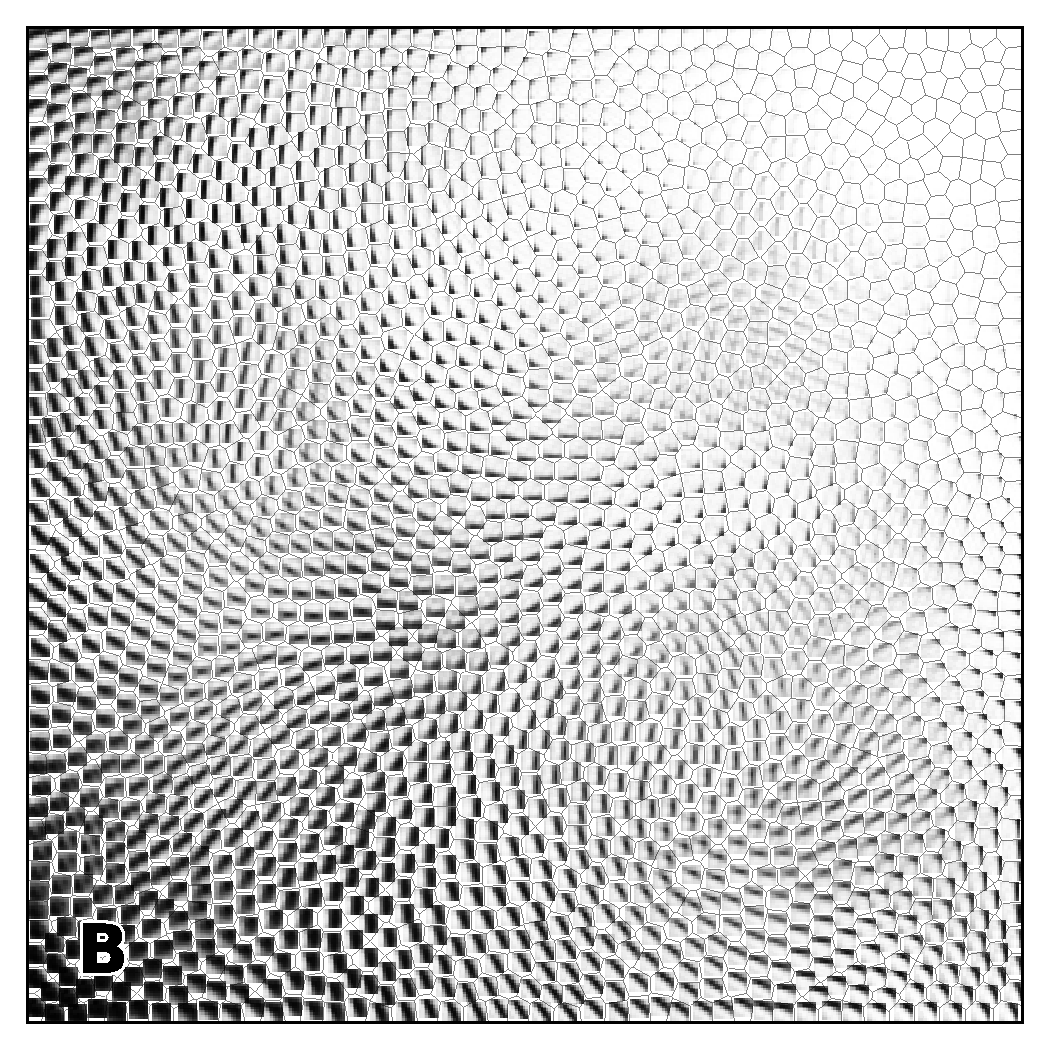
\includegraphics[width=\textwidth]{figures/vsom-image-1.pdf}
  
  \vspace{2mm}

  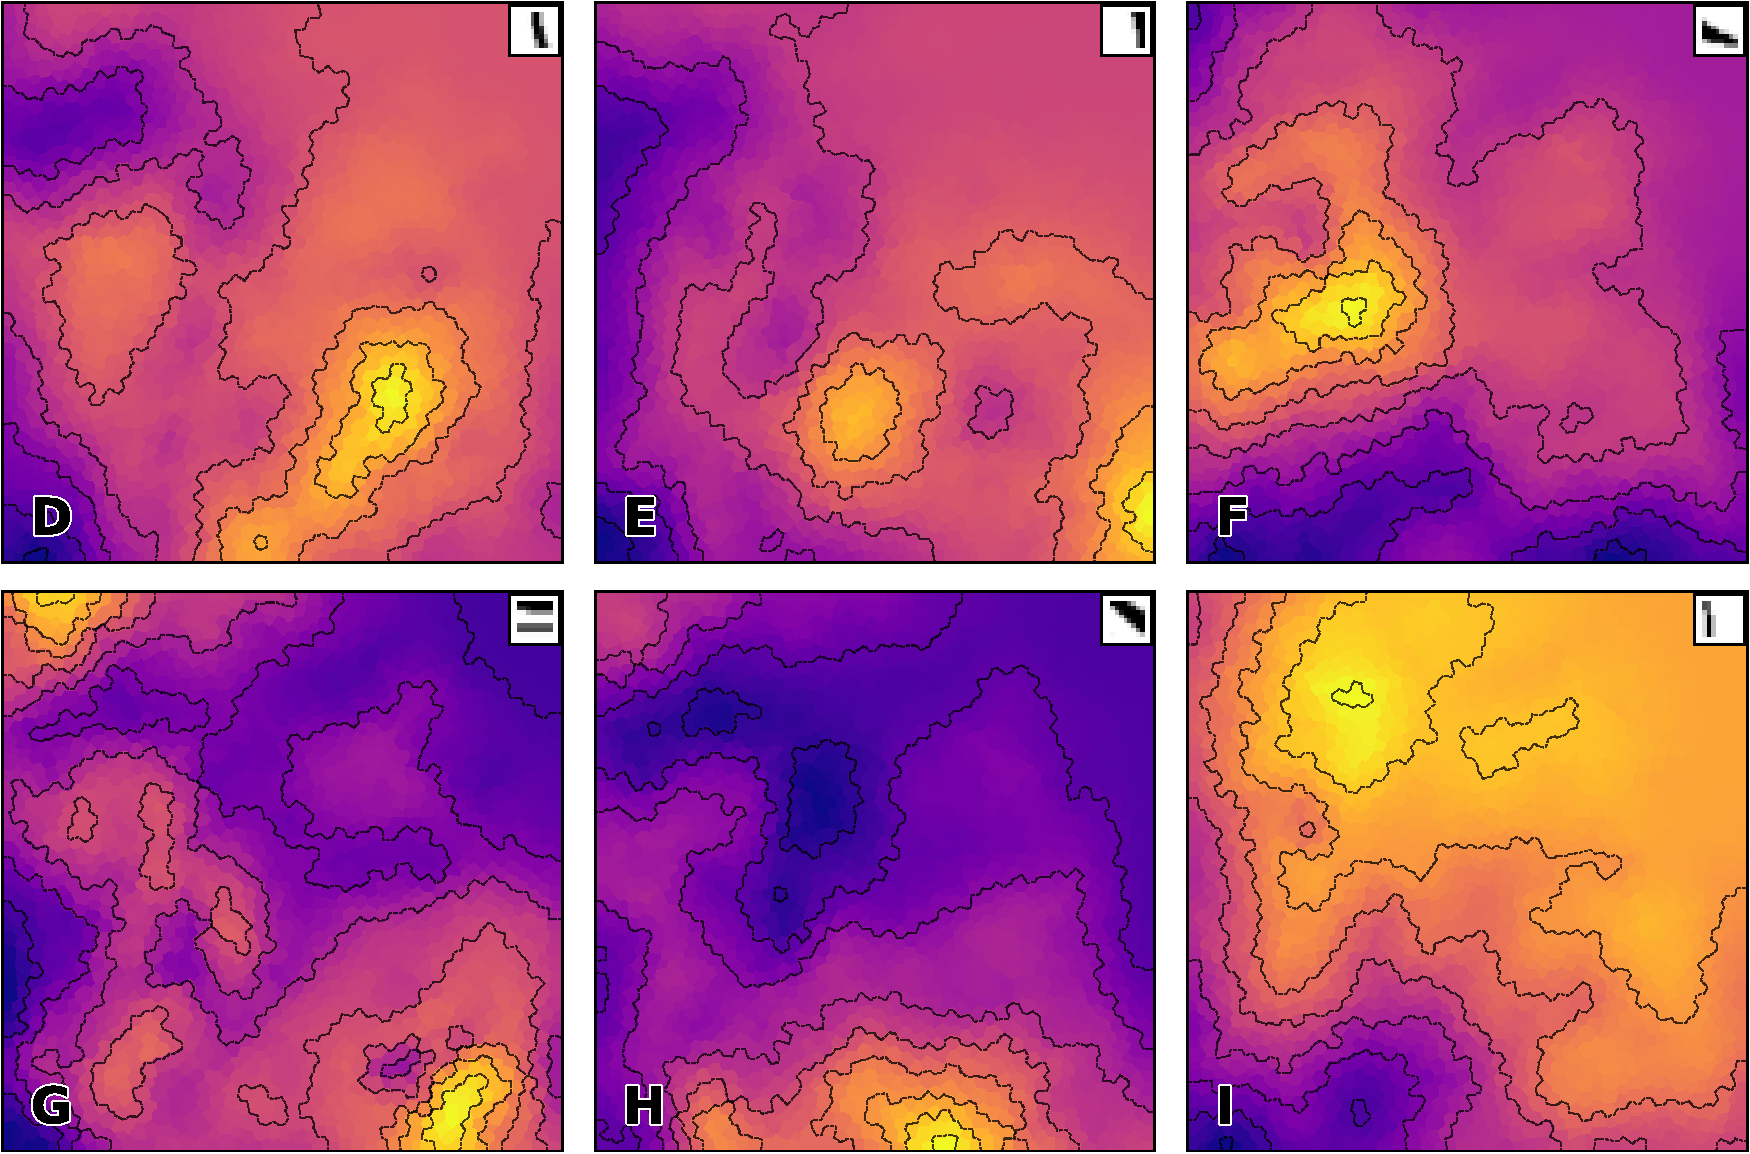
\includegraphics[width=\textwidth]{figures/vsom-image-2.pdf}

  \caption{Voronoidal SOM made of 1003 neurons with a 2-nearest neighbors
    induced topology. Model has been trained for 10,000 epochs on random
    uniform scalars in [0,1]. \textbf{A} Map topology in the neural
    space. \textbf{B} Map prototypes displayed in neural space using Voronoi
    cells (whose color indicates prototype according to colormap). \textbf{C to
      H} Map activity for some random data (\textbf{C}:0.0, \textbf{D}:0.2,
    \textbf{E}: 0.4, \textbf{F}:0.6, \textbf{G}:0.8, \textbf{H}:1.0).}
\end{figure}


\subsection{Reorganization}

In case of neural loss (a set of neurons is removed from the map) or neural
gain (a set of neurons is added to the map), we can appy the LLoyd relaxation
scheme in order to achieve a new quasi centroidal Voronoi tesselation (see
figure \ref{fig:CVT}) whose induced topology shares similarity with the orginal
topology (before loss or gain).

\begin{figure}
  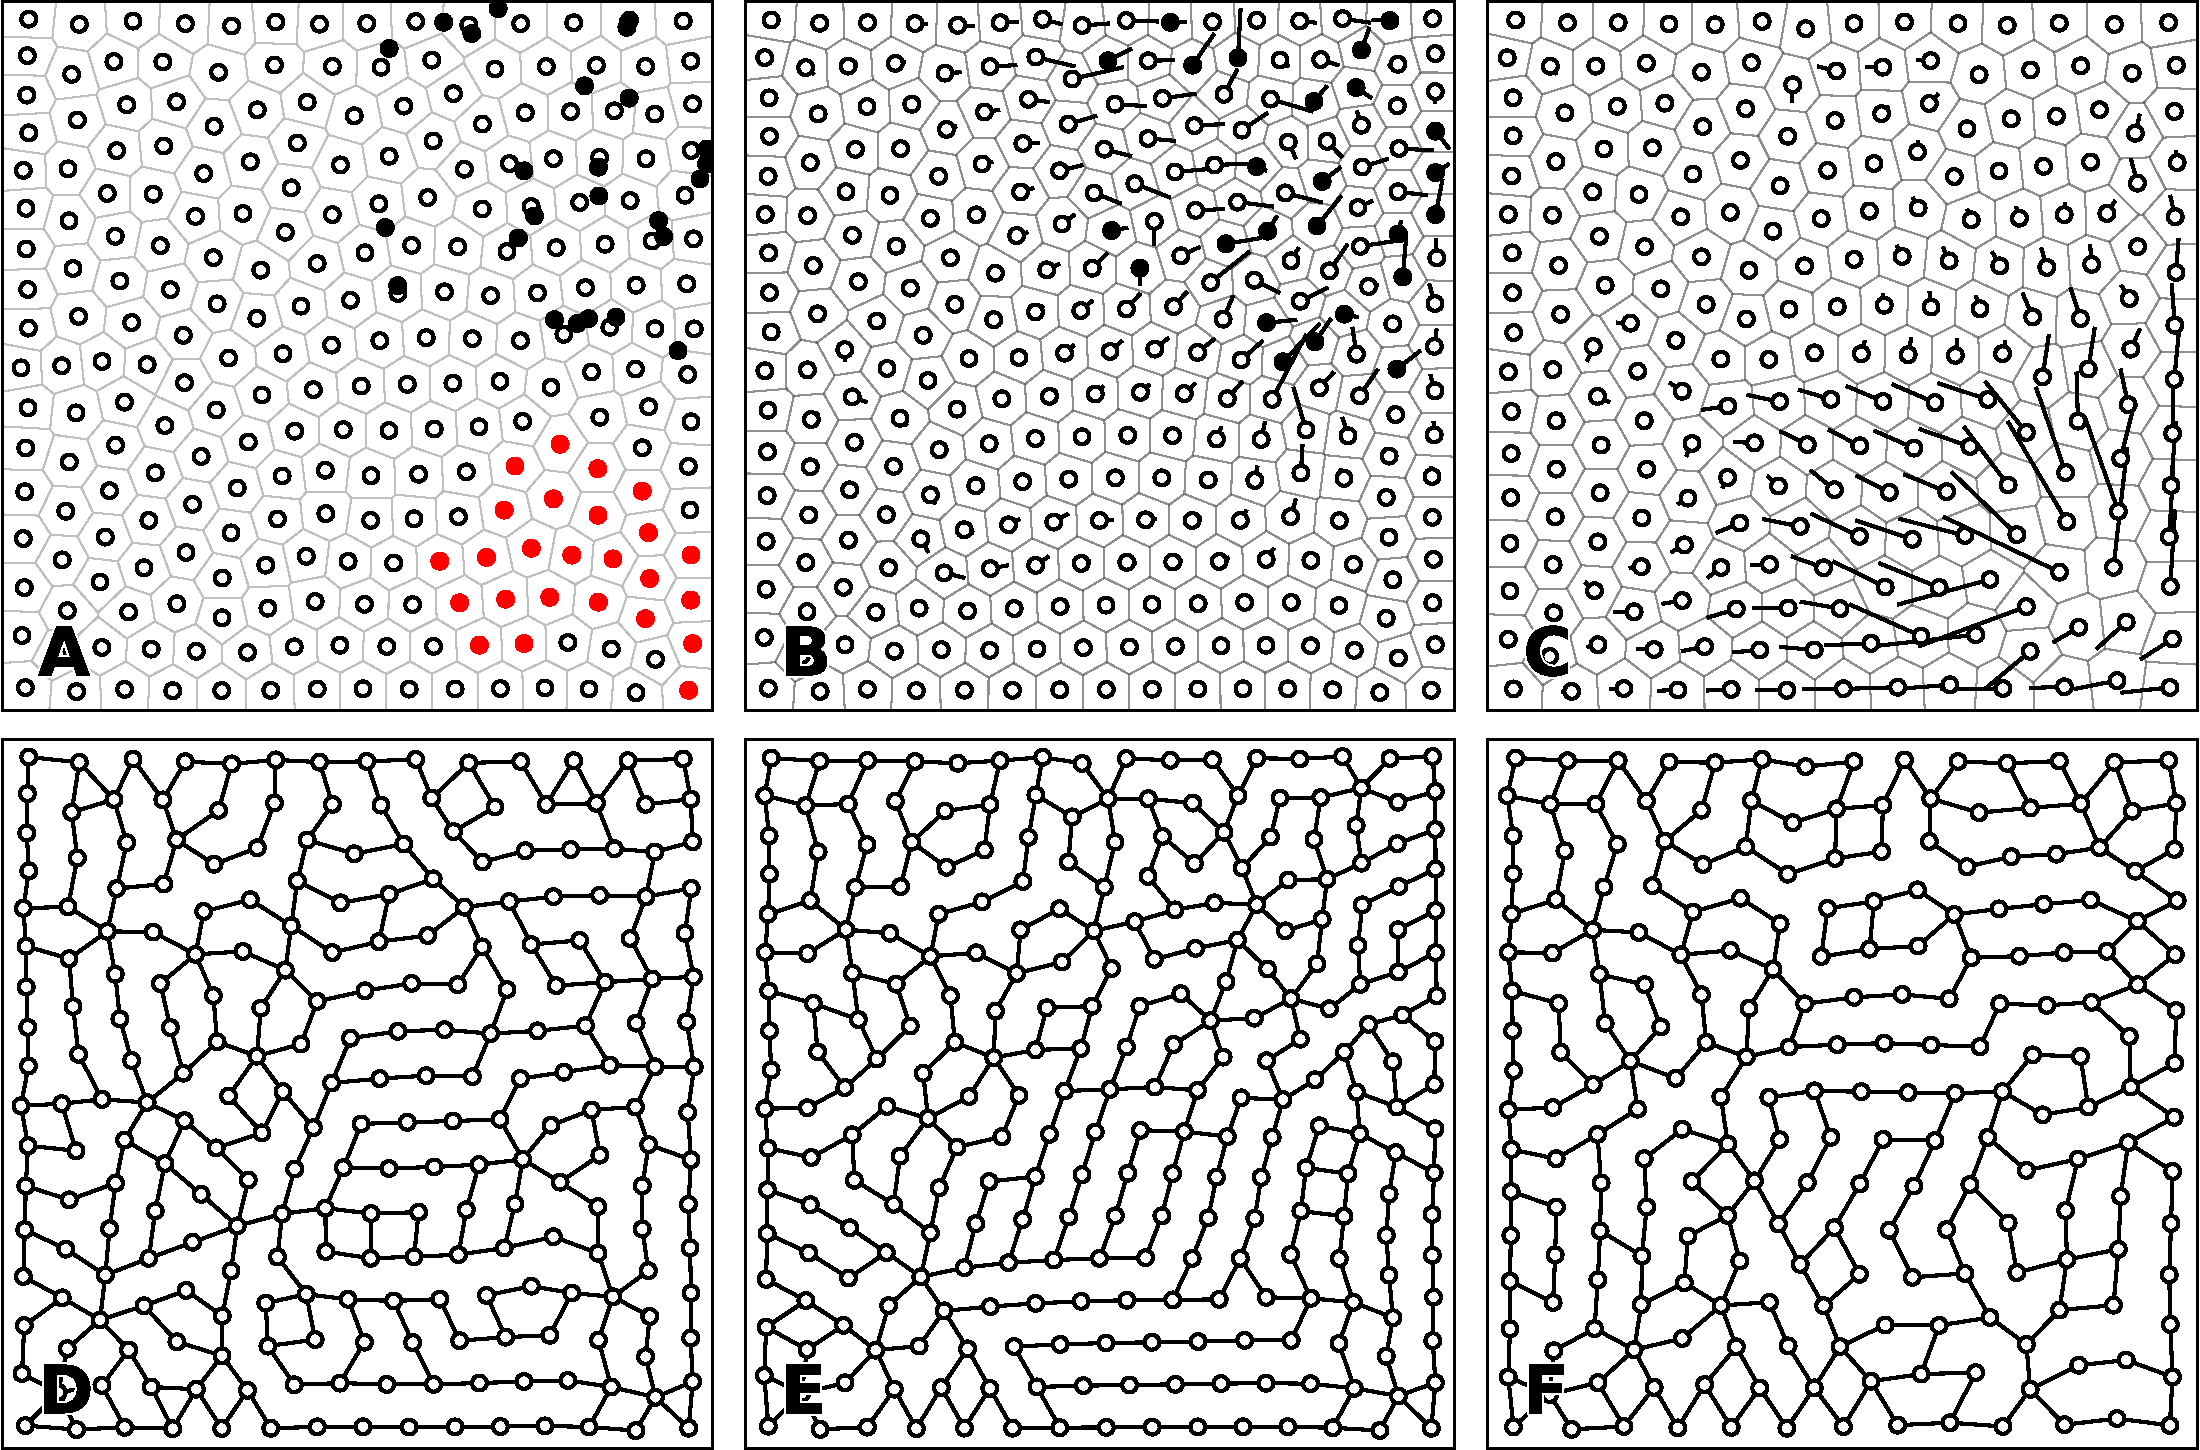
\includegraphics[width=\columnwidth]{figures/vsom-resilience.pdf}
  \caption{\textbf{Reorganization following neural loss or gain.}  An initial
    set of 248 neurons (outlined discs on panel \textbf{A}) has been modified
    with the addition of 25 neurons (black discs) or the removal of 25 neurons
    (red discs). Panels \textbf{B} and \textbf{C} show the final position of
    neurons after 100 iterations of the centroidal Voronoi tesselation. Lines
    shows individual movement of neurons. Panels \textbf{D}, \textbf{E} and
    \textbf{F} show the 2-neighbors induced topology for \textbf{A},
    \textbf{B} and \textbf{C} respectively.}
  \label{fig:CVT}
\end{figure}

\subsubsection*{Ablation}

\subsubsection*{Addition}

\section{Conclusion}

This article comes last in a series of three articles where we investigate for
a more biologically plausible self-organization. 





\section*{Abbreviations}
\begin{description}
    \item[\bf SOM] Self-organizing Map
    \item[\bf BMU] Best matching unit
    \item[\bf DSOM] Dynamic Self-organizing Map
\end{description}





%% \begin{figure}
%%   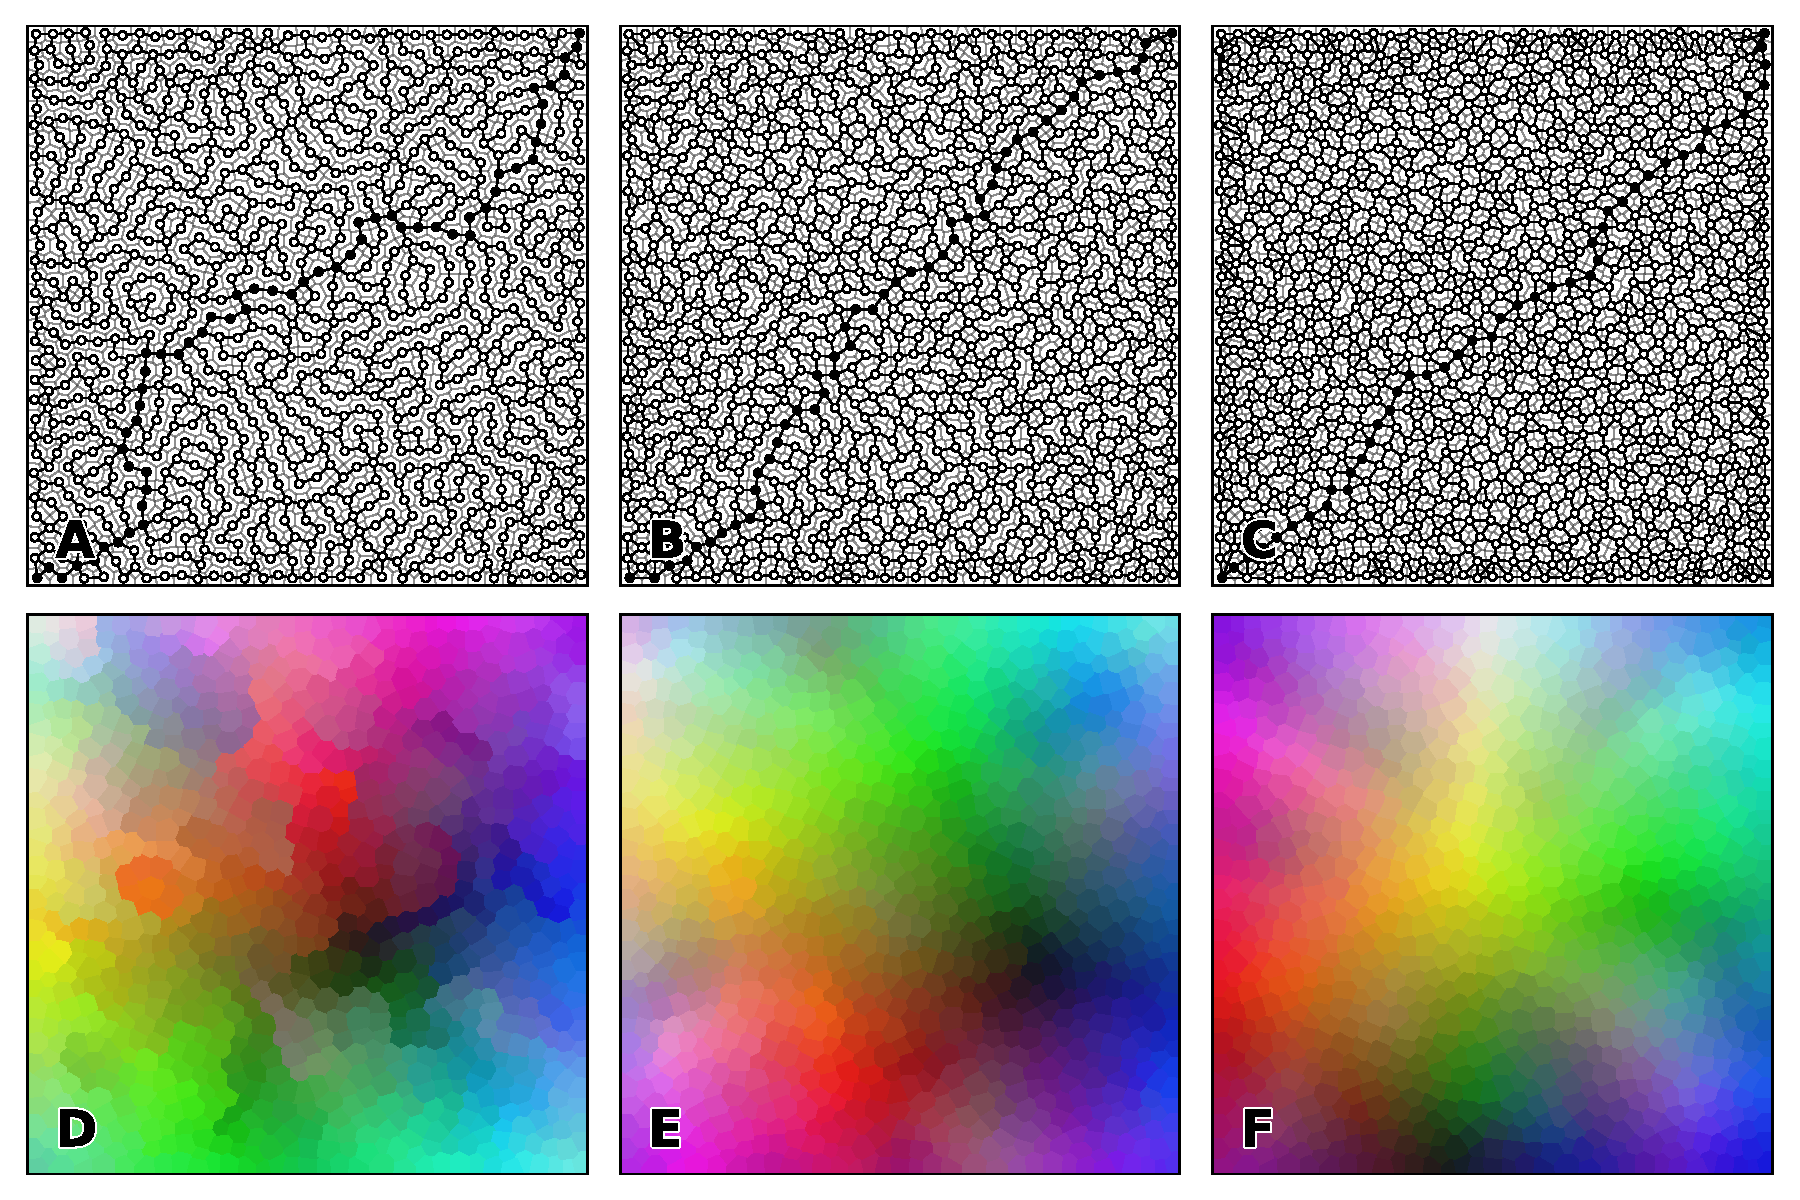
\includegraphics[width=\columnwidth]{figures/vsom-topology.pdf}

%%   \caption{\textbf{Influence of topology on the self organization.} The same
%%     initial set of 1003 neurons has been equiped with 2-nearest neighbors, 3
%%     nearest neighbors and 4-nearest neighbors induced topology (panels
%%     \textbf{A}, \textbf{B} and \textbf{C} respectively) and trained on 25,000
%%     random RGB colors. This lead to qualitatively different self-organization
%%     as shown on panels \textbf{D}, \textbf{E} and \textbf{F} respectively, with
%%     major discontinuities in the 2-nearest neighbors case. A sample path from
%%     the the lower-left neuron to the upper-right neuron has been highlighted with
%%     a thick line (with respective lengths of 59, 50 and 46 nodes).}
%% \end{figure}

%% \begin{figure}
%%   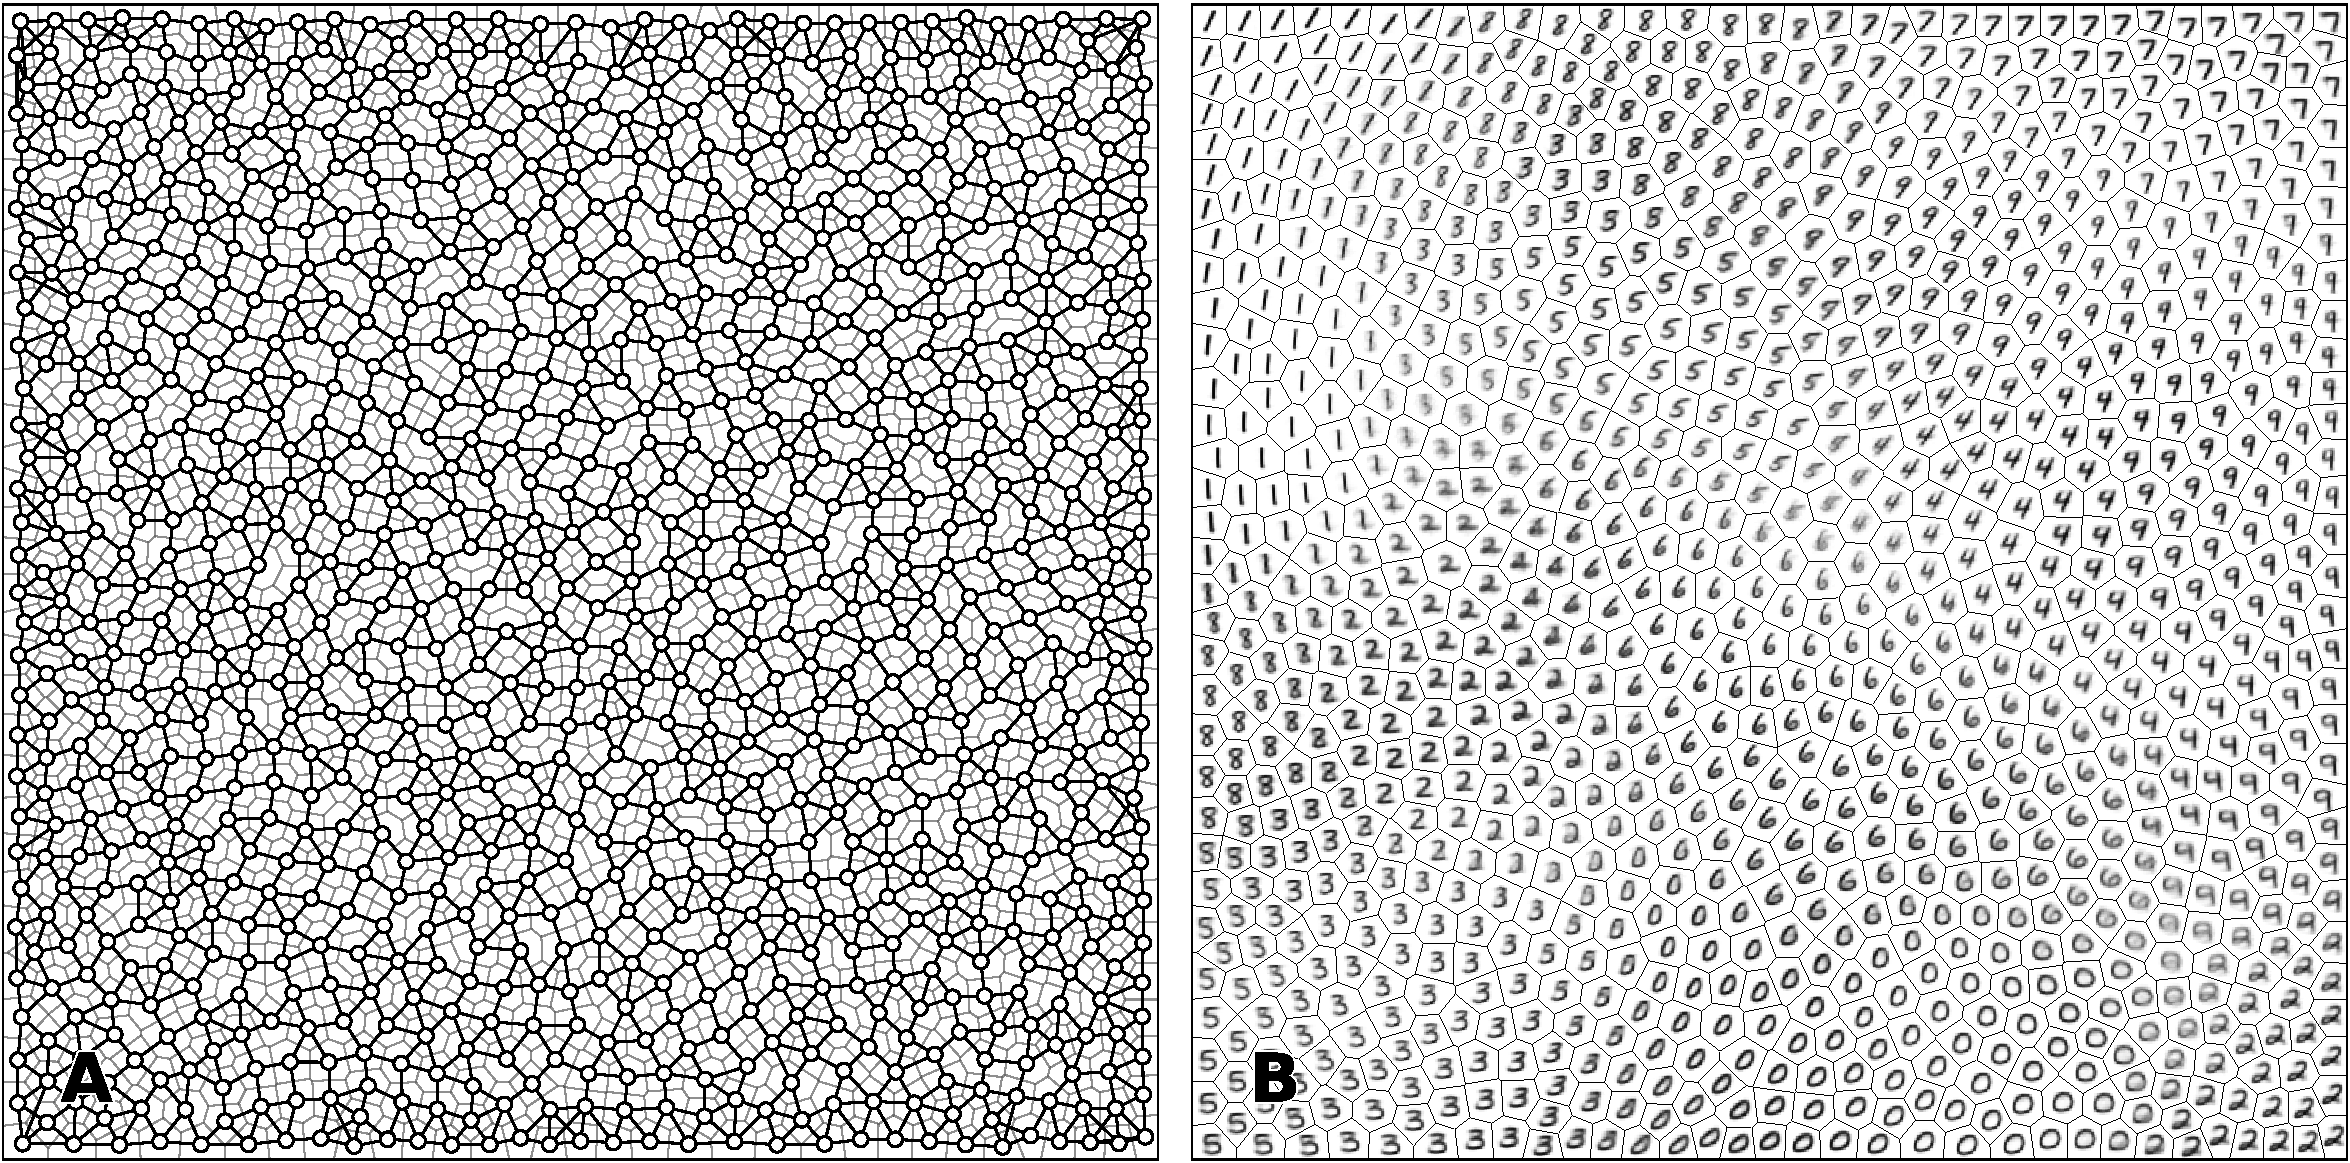
\includegraphics[width=\columnwidth]{figures/vsom-mnist-1.pdf}

%%   \vspace{2mm}
  
%%   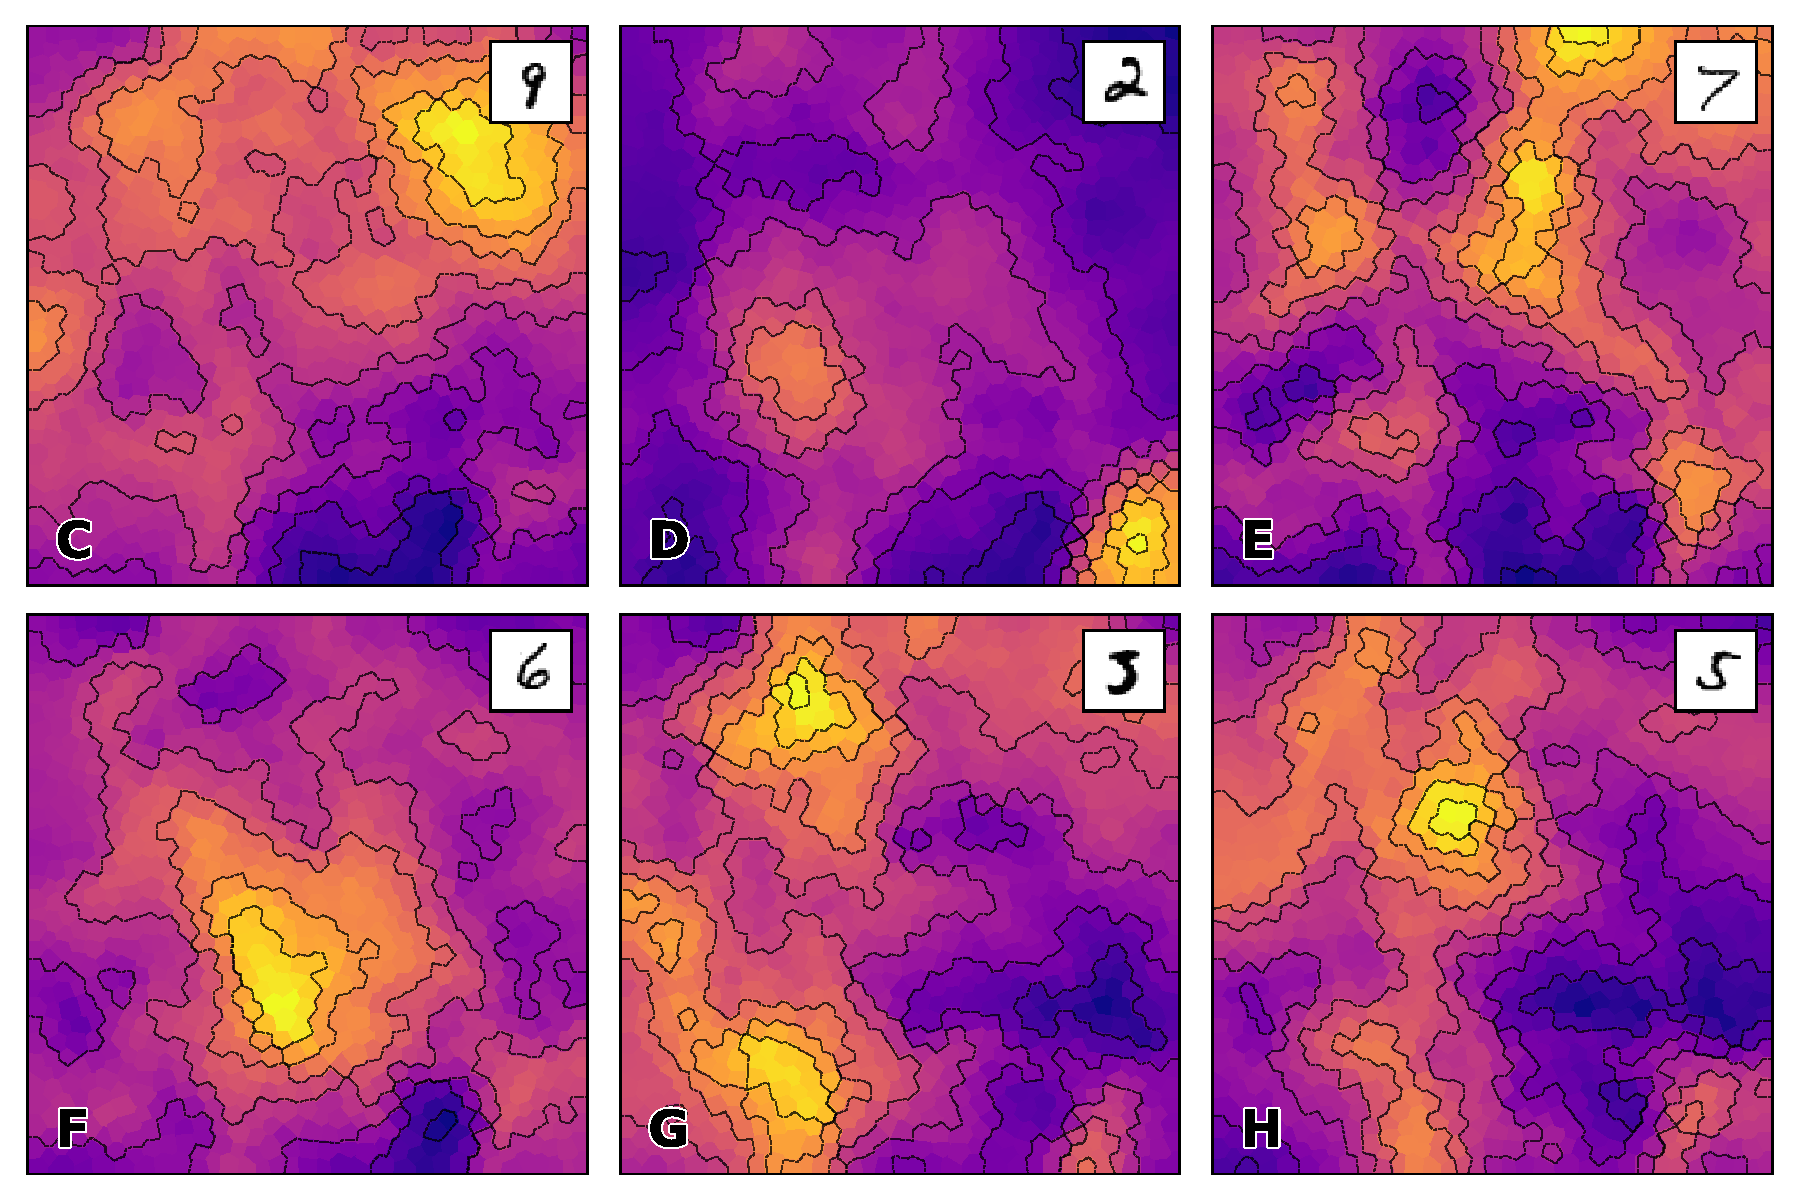
\includegraphics[width=\columnwidth]{figures/vsom-mnist-2.pdf}

%%   \vspace{2mm}

%%   \includegraphics[width=\columnwidth]{figures/colormap.pdf}

%%   \caption{}
%% \end{figure}


%% \begin{figure}
%%   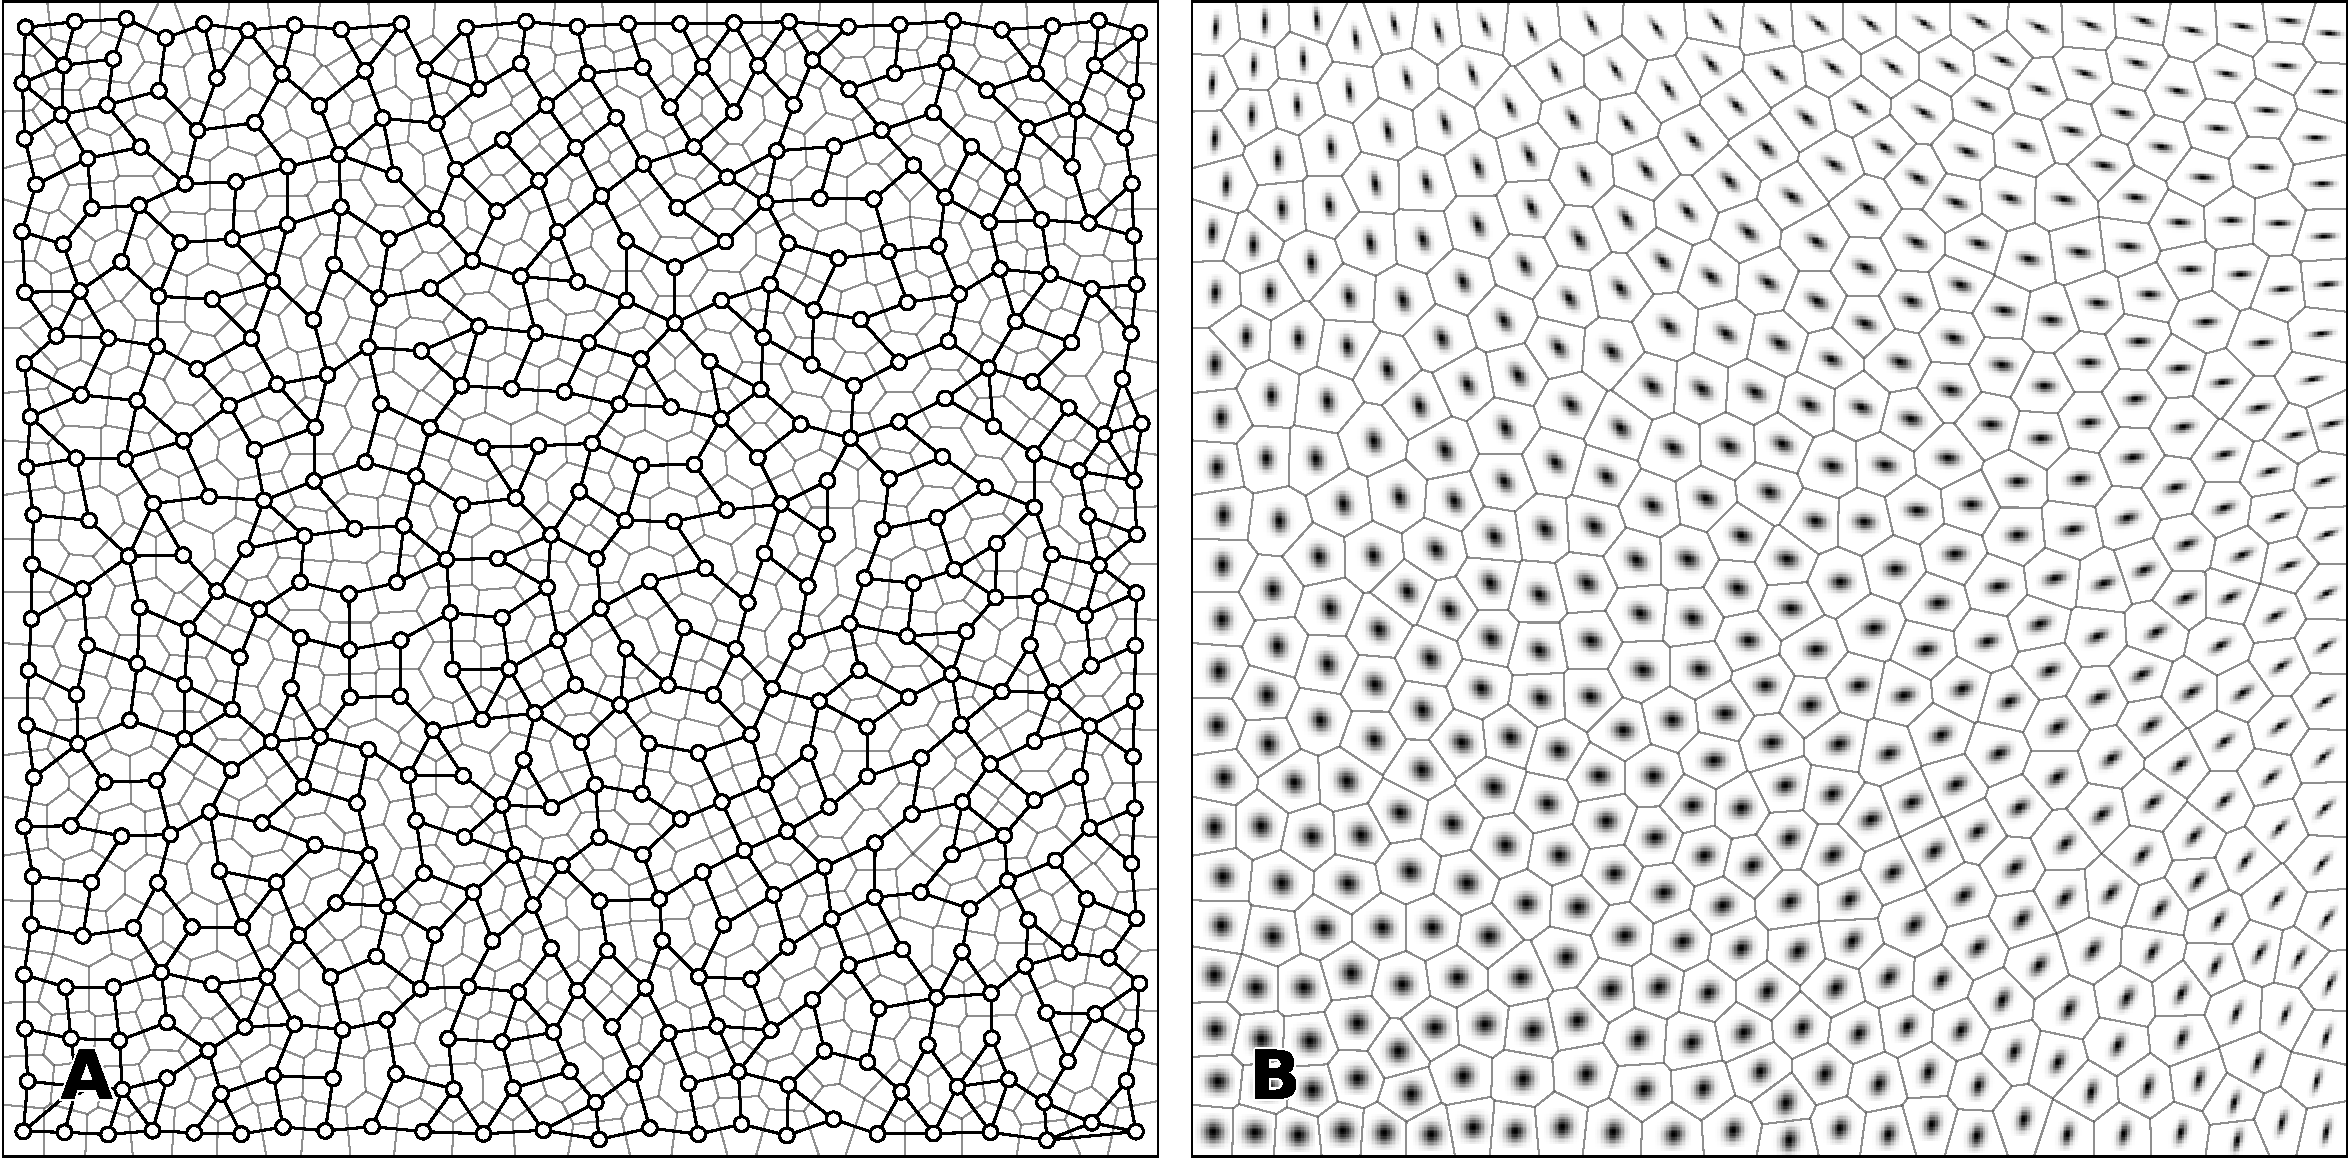
\includegraphics[width=\columnwidth]{figures/vsom-gaussian-1.pdf}
  
%%   \vspace{2mm}
  
%%   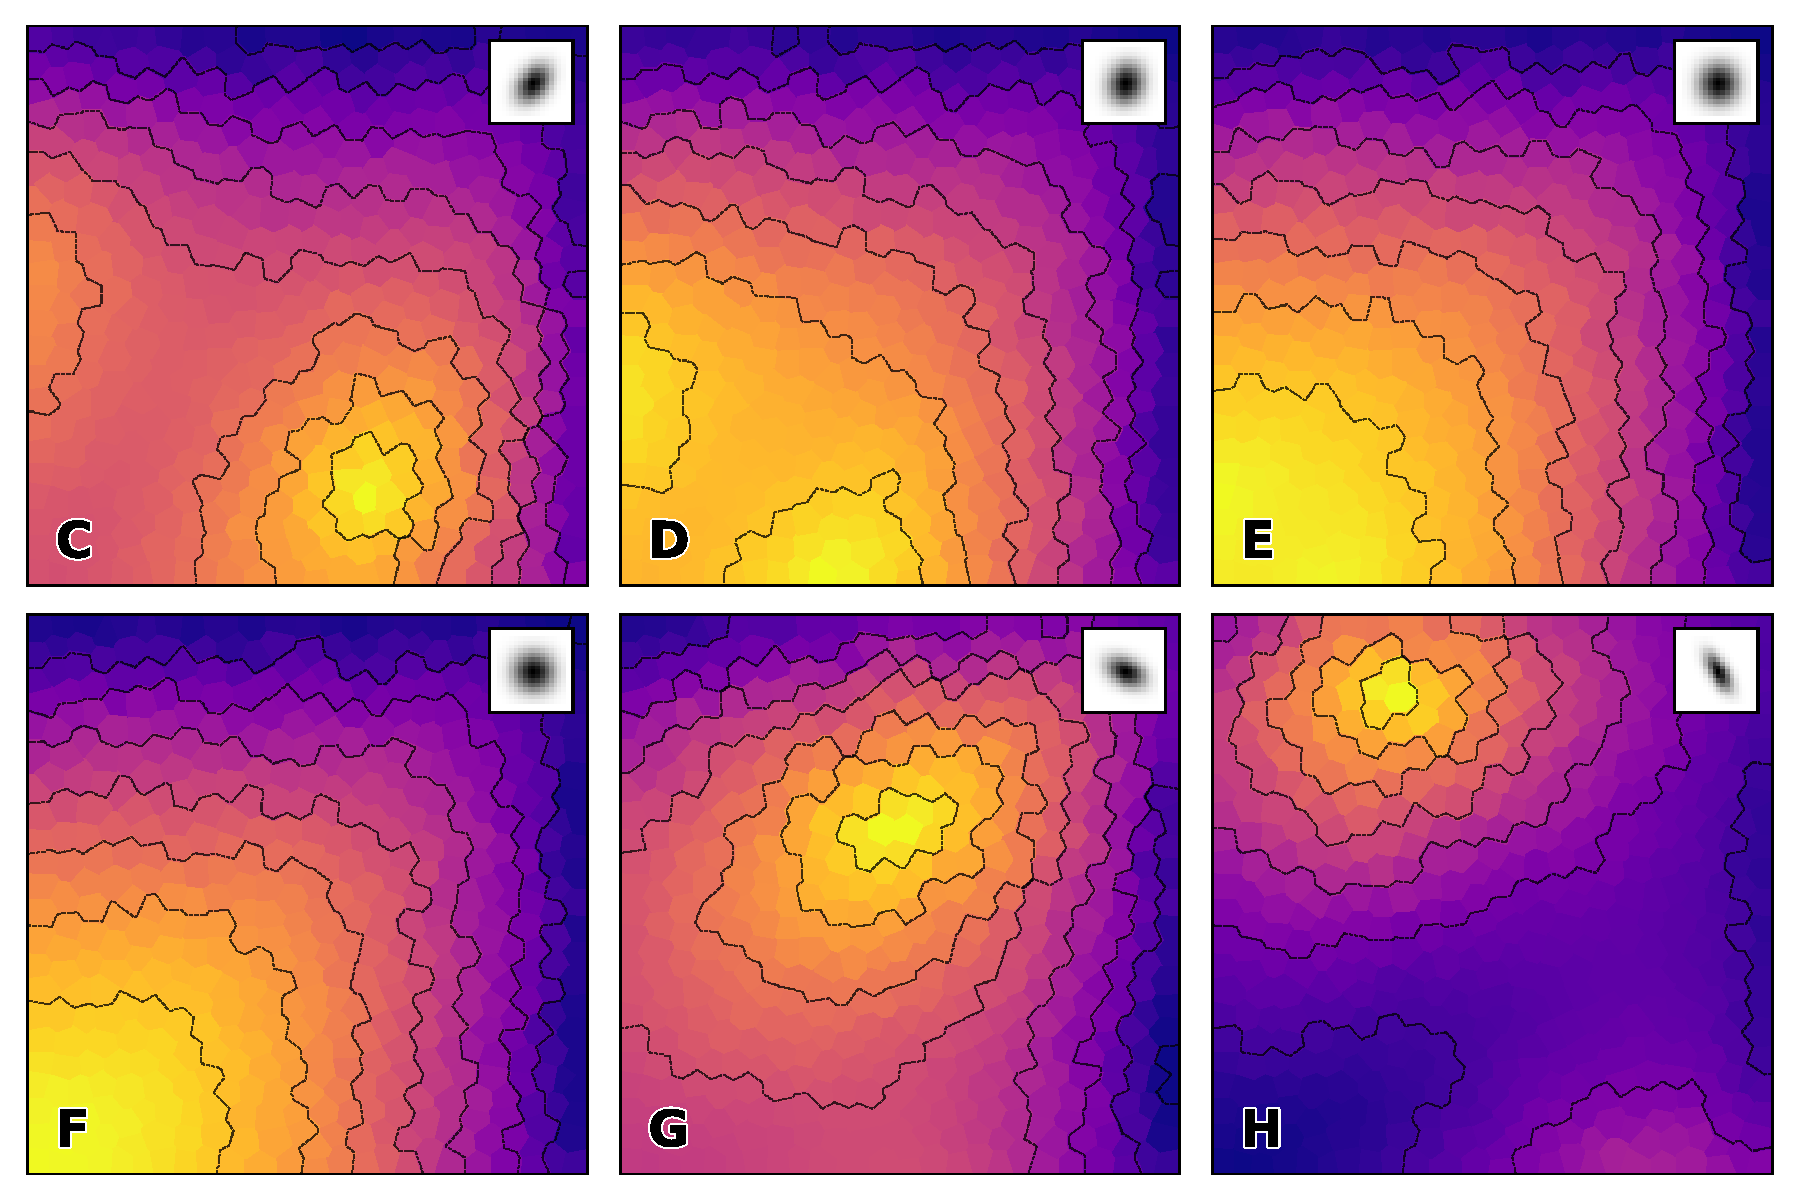
\includegraphics[width=\columnwidth]{figures/vsom-gaussian-2.pdf}

%%   \vspace{2mm}

%%   \includegraphics[width=\columnwidth]{figures/colormap.pdf}

%%   \caption{}
%% \end{figure}


\section*{Abbreviations}
\begin{description}
    \item[BMU]     Best Matching unit
    \item[DNF-SOM] Dynamic Neural Field-Self-Organizing Map
    \item[DSOM]    Dynamic Self-organizing Map
    \item[KSOM]    Kohonen Self-Organizing Map (Kohonen original proposal)
    \item[KDE]     Kernel Density Estimation
    \item[RSOM]    Randomized Self-Organizing Map
    \item[TDA]     Topological Data Analysis
    \item[SOM]     Self-Organizing Map
\end{description}

\section*{Funding}
This work was partially funded by grant ANR-17-CE24-0036.

\bibliographystyle{apa}
\bibliography{biblio}

% \printbibliography %[heading=bibintoc]


\newpage
\appendix
\section{Supplementary material}

Randomized Self Organizing Map \\ 
Nicolas P. Rougier$^{1,2,3}$ and Georgios Is. Detorakis$^4$ \\
$^1$ Inria Bordeaux Sud-Ouest \\
$^2$ Institut des Maladies Neurodégénératives, Université  de Bordeaux, CNRS UMR 5293 \\
$^3$ LaBRI, Université de Bordeaux, Institut Polytechnique de Bordeaux, CNRS UMR 5800 \\
$^4$ adNomus Inc., San Jose, CA, USA \\
\medskip
% Self-organizing maps usually rely on a predetermined topology of the neural space (the map), which is either a rectangular or a hexagonal Cartesian grid. When the intrinsic dimension of  the input space is much higher than the allowed dimension of the neural space, then the self-organizing map can be ill-formed. To overcome this problem in  high dimensional input spaces. We propose a variation of the self organizing map algorithm, where we consider random placement of neurons on a high-dimensional manifold. The positions of the neural units are drawn from a blue noise distribution from which various topologies can be derived. These topologies possess  random but controllable discontinuities that allow for a flexible self-organization, especially with high-dimensional data. The proposed algorithm has been tested on one-, two- and three-dimensions tasks as well as on MNIST handwritten digits dataset. Furthermore, we investigate the reorganization of the self-organizing maps when we either remove or add neurons to the map. To analyze the results we use spectral analysis and topological data analysis tools. 
%

\textbf{Abstract.} We propose a variation of the self organizing map algorithm by considering the random placement of neurons on a two-dimensional manifold, following a blue noise distribution from which various topologies can be derived. These topologies possess random (but controllable) discontinuities that allow for a more flexible self-organization, especially with high-dimensional data. The proposed algorithm is tested on one-, two- and three-dimensions tasks as well as on the MNIST handwritten digits dataset and validated using spectral analysis and topological data analysis tools. We also demonstrate the ability of the randomized self-organizing map to gracefully reorganize itself in case of neural lesion and/or neurogenesis.\par

% \textbf{Keywords.} Self Organization, Neural Networks, Vector Quantization, Voronoi Tesselation, Neural Map Topology

\bigskip


\subsection{One-dimensional uniform dataset}

% We train a two-dimensional map over $25000$ samples drawn from a uniform distribution ($\mathcal{U}(0, 1)$). The map consists of $1024$ units (neurons) and it is being trained for $25000$ epochs (all the parameters can be found in Table~\ref{table:parameters}). Figure~\ref{fig:one-dim}{\bfseries \sffamily A} shows the neural space topology of the two-dimensional map after sampling a blue noise distribution and placing the neurons on the corresponding nodes. Figure~\ref{fig:one-dim}{\bfseries \sffamily B} indicates the learned representations after training. In this case the mapping of real numbers within the interval $[0, 1]$ is illustrated in color-code with blue color representing number zero and yellow representing one. It is clear that the map has organize the representations in a descending order starting from the upper left corner (one) of the map to the lower right corner (zero).

% Neurons of both the Kohonen and VSOM maps develop receptive filters during training. Each of these receptive fields usually captures a portion of the input space and learns the reciprocal representations. Therefore, we examine the receptive fields of neurons by evaluating their response to a stimulus. To this end, we feed the map with $6$ input samples after discretizing the interval $[0, 1]$. The activity of each neuron is  computed as the Euclidean distance between the input sample and the neuron's code word. Figures~\ref{fig:one-dim} {\sffamily \bfseries C}-{\sffamily \bfseries H}  show the neural activity on the map for $6$ input samples. It is apparent that different regions of the map respond to different stimuli, implying that the topographic organization has been successfully accomplished. 


\begin{figure}
  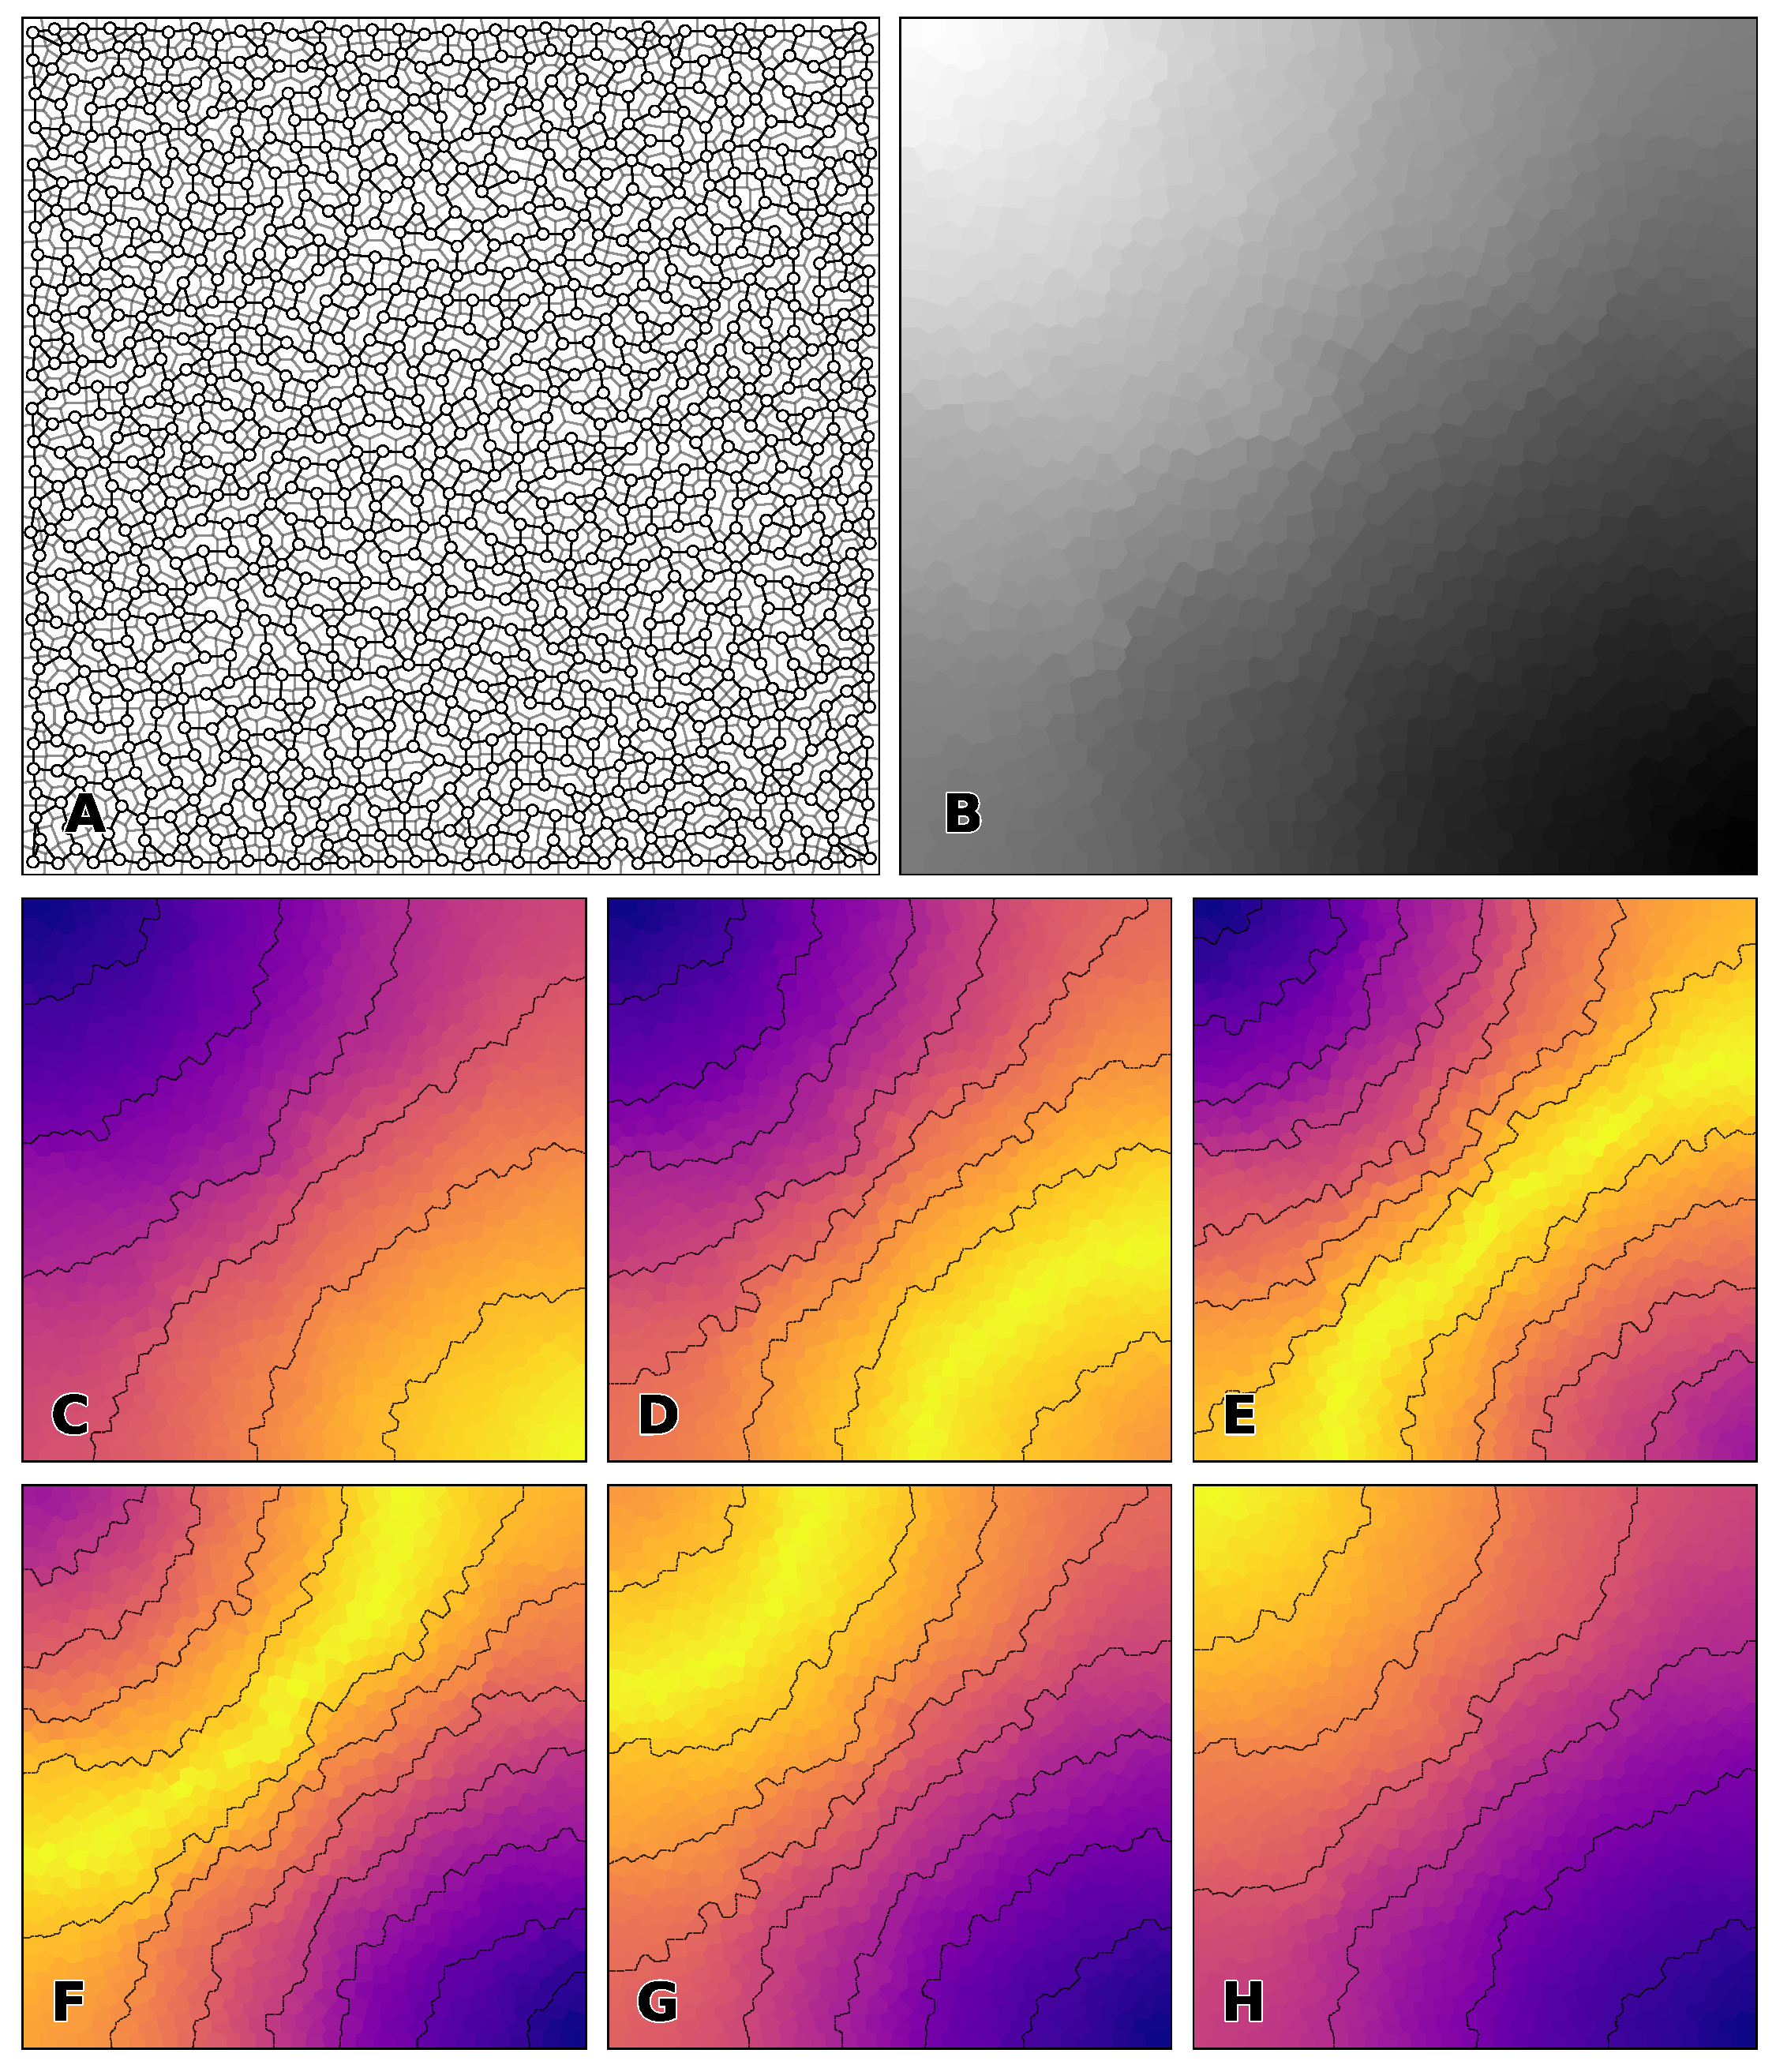
\includegraphics[width=\columnwidth]{experiment-1D-uniform.pdf}
  \vspace{2mm}
  \centering
  \includegraphics[width=.975\columnwidth]{figures/colormap.pdf}
  %
  \caption{%
  %
  {\bfseries \sffamily One dimensional uniform dataset with holes (results)}
  %
  Randomized SOM made of $1024$ neurons with a $3$-nearest neighbors induced topology. Model has been trained for $25,000$ epochs on one-dimensional points drawn from a uniform distribution on the unit segment. \textbf{A} Map topology in neural space. \textbf{B} Map topology in data space. \textbf{C to H} Receptive field of the map for six samples.
  %
  }
  \label{fig:1D-uniform:results}
\end{figure}


\subsection{Two dimensional uniform dataset}

\begin{figure}
  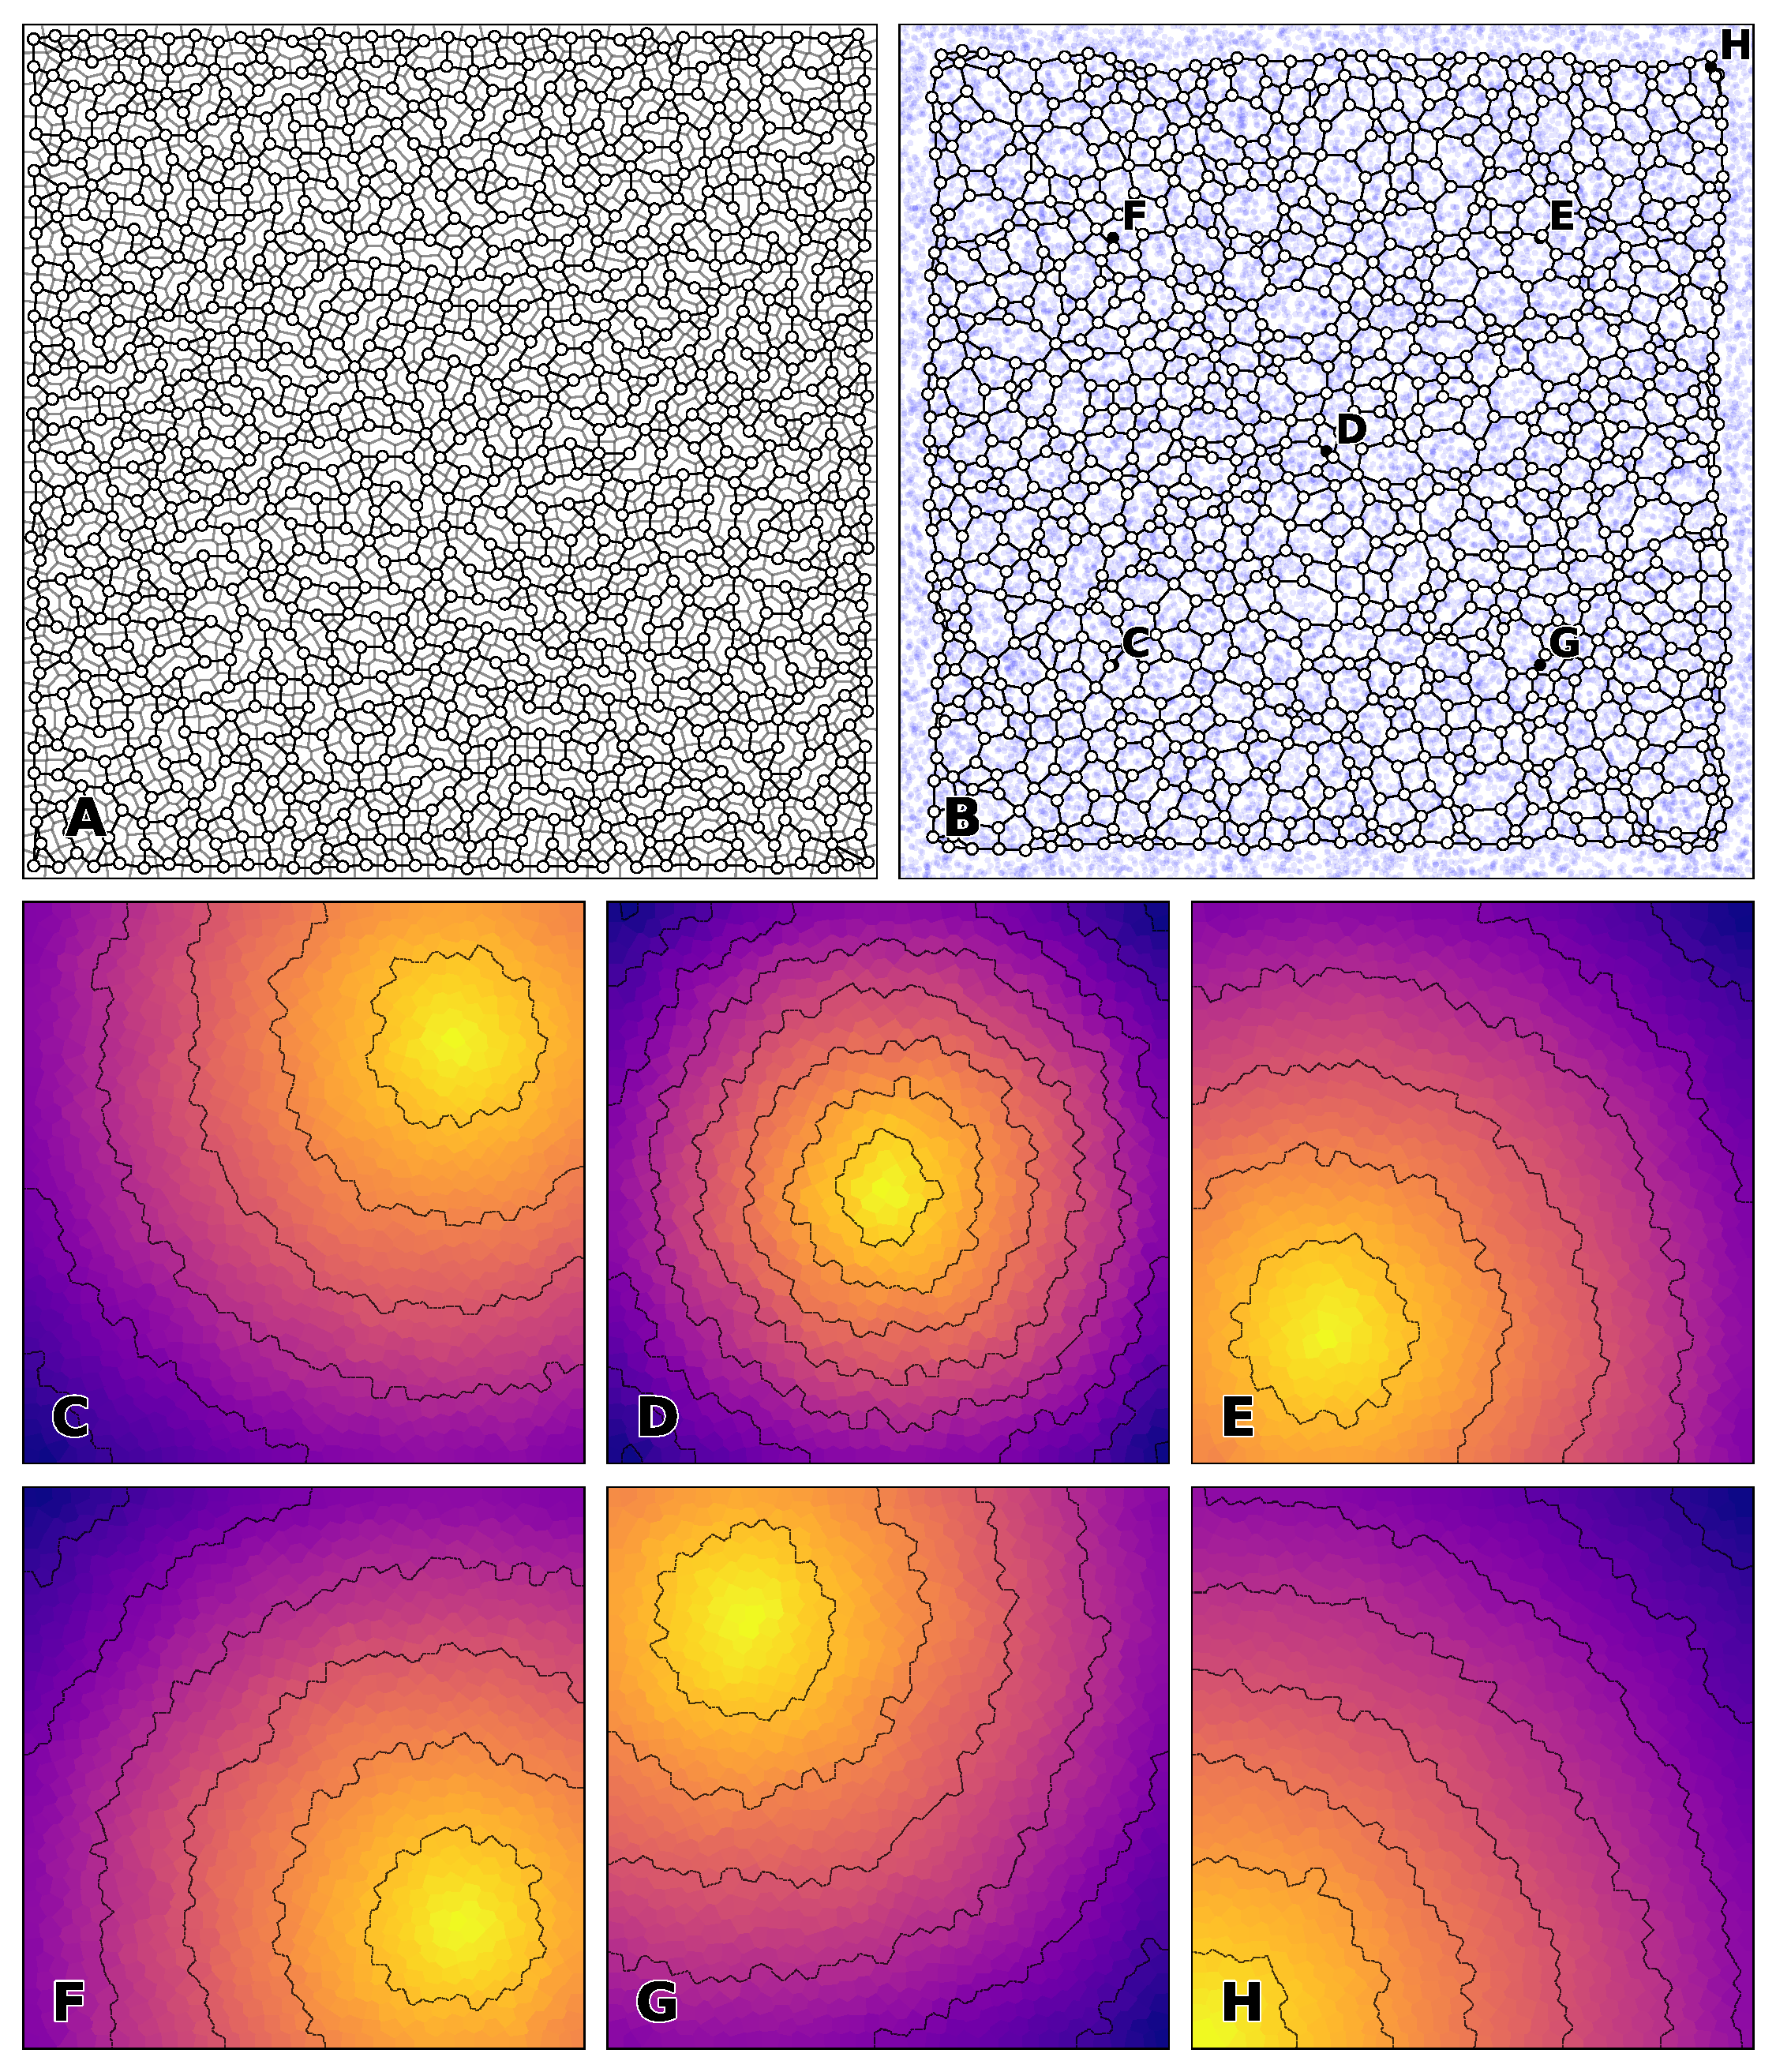
\includegraphics[width=\columnwidth]{experiment-2D-uniform.pdf}
  \vspace{2mm}
  \centering
  \includegraphics[width=.975\columnwidth]{colormap.pdf}
  %
  \caption{%
  %
  {\bfseries \sffamily Two dimensional uniform dataset (results)}
  %
  Randomized SOM made of $1024$ neurons with a $2$-nearest neighbors induced topology. Model has been trained for $25,000$ epochs on two-dimensional points drawn from a uniform distribution on the unit square. \textbf{A} Map topology in neural space. \textbf{B} Map topology in data space. \textbf{C to H} Receptive field of the map for six samples.
  %
  }
  \label{fig:2D-uniform:results}
\end{figure}

\subsection{Two-dimensional ring dataset }

\begin{figure}
  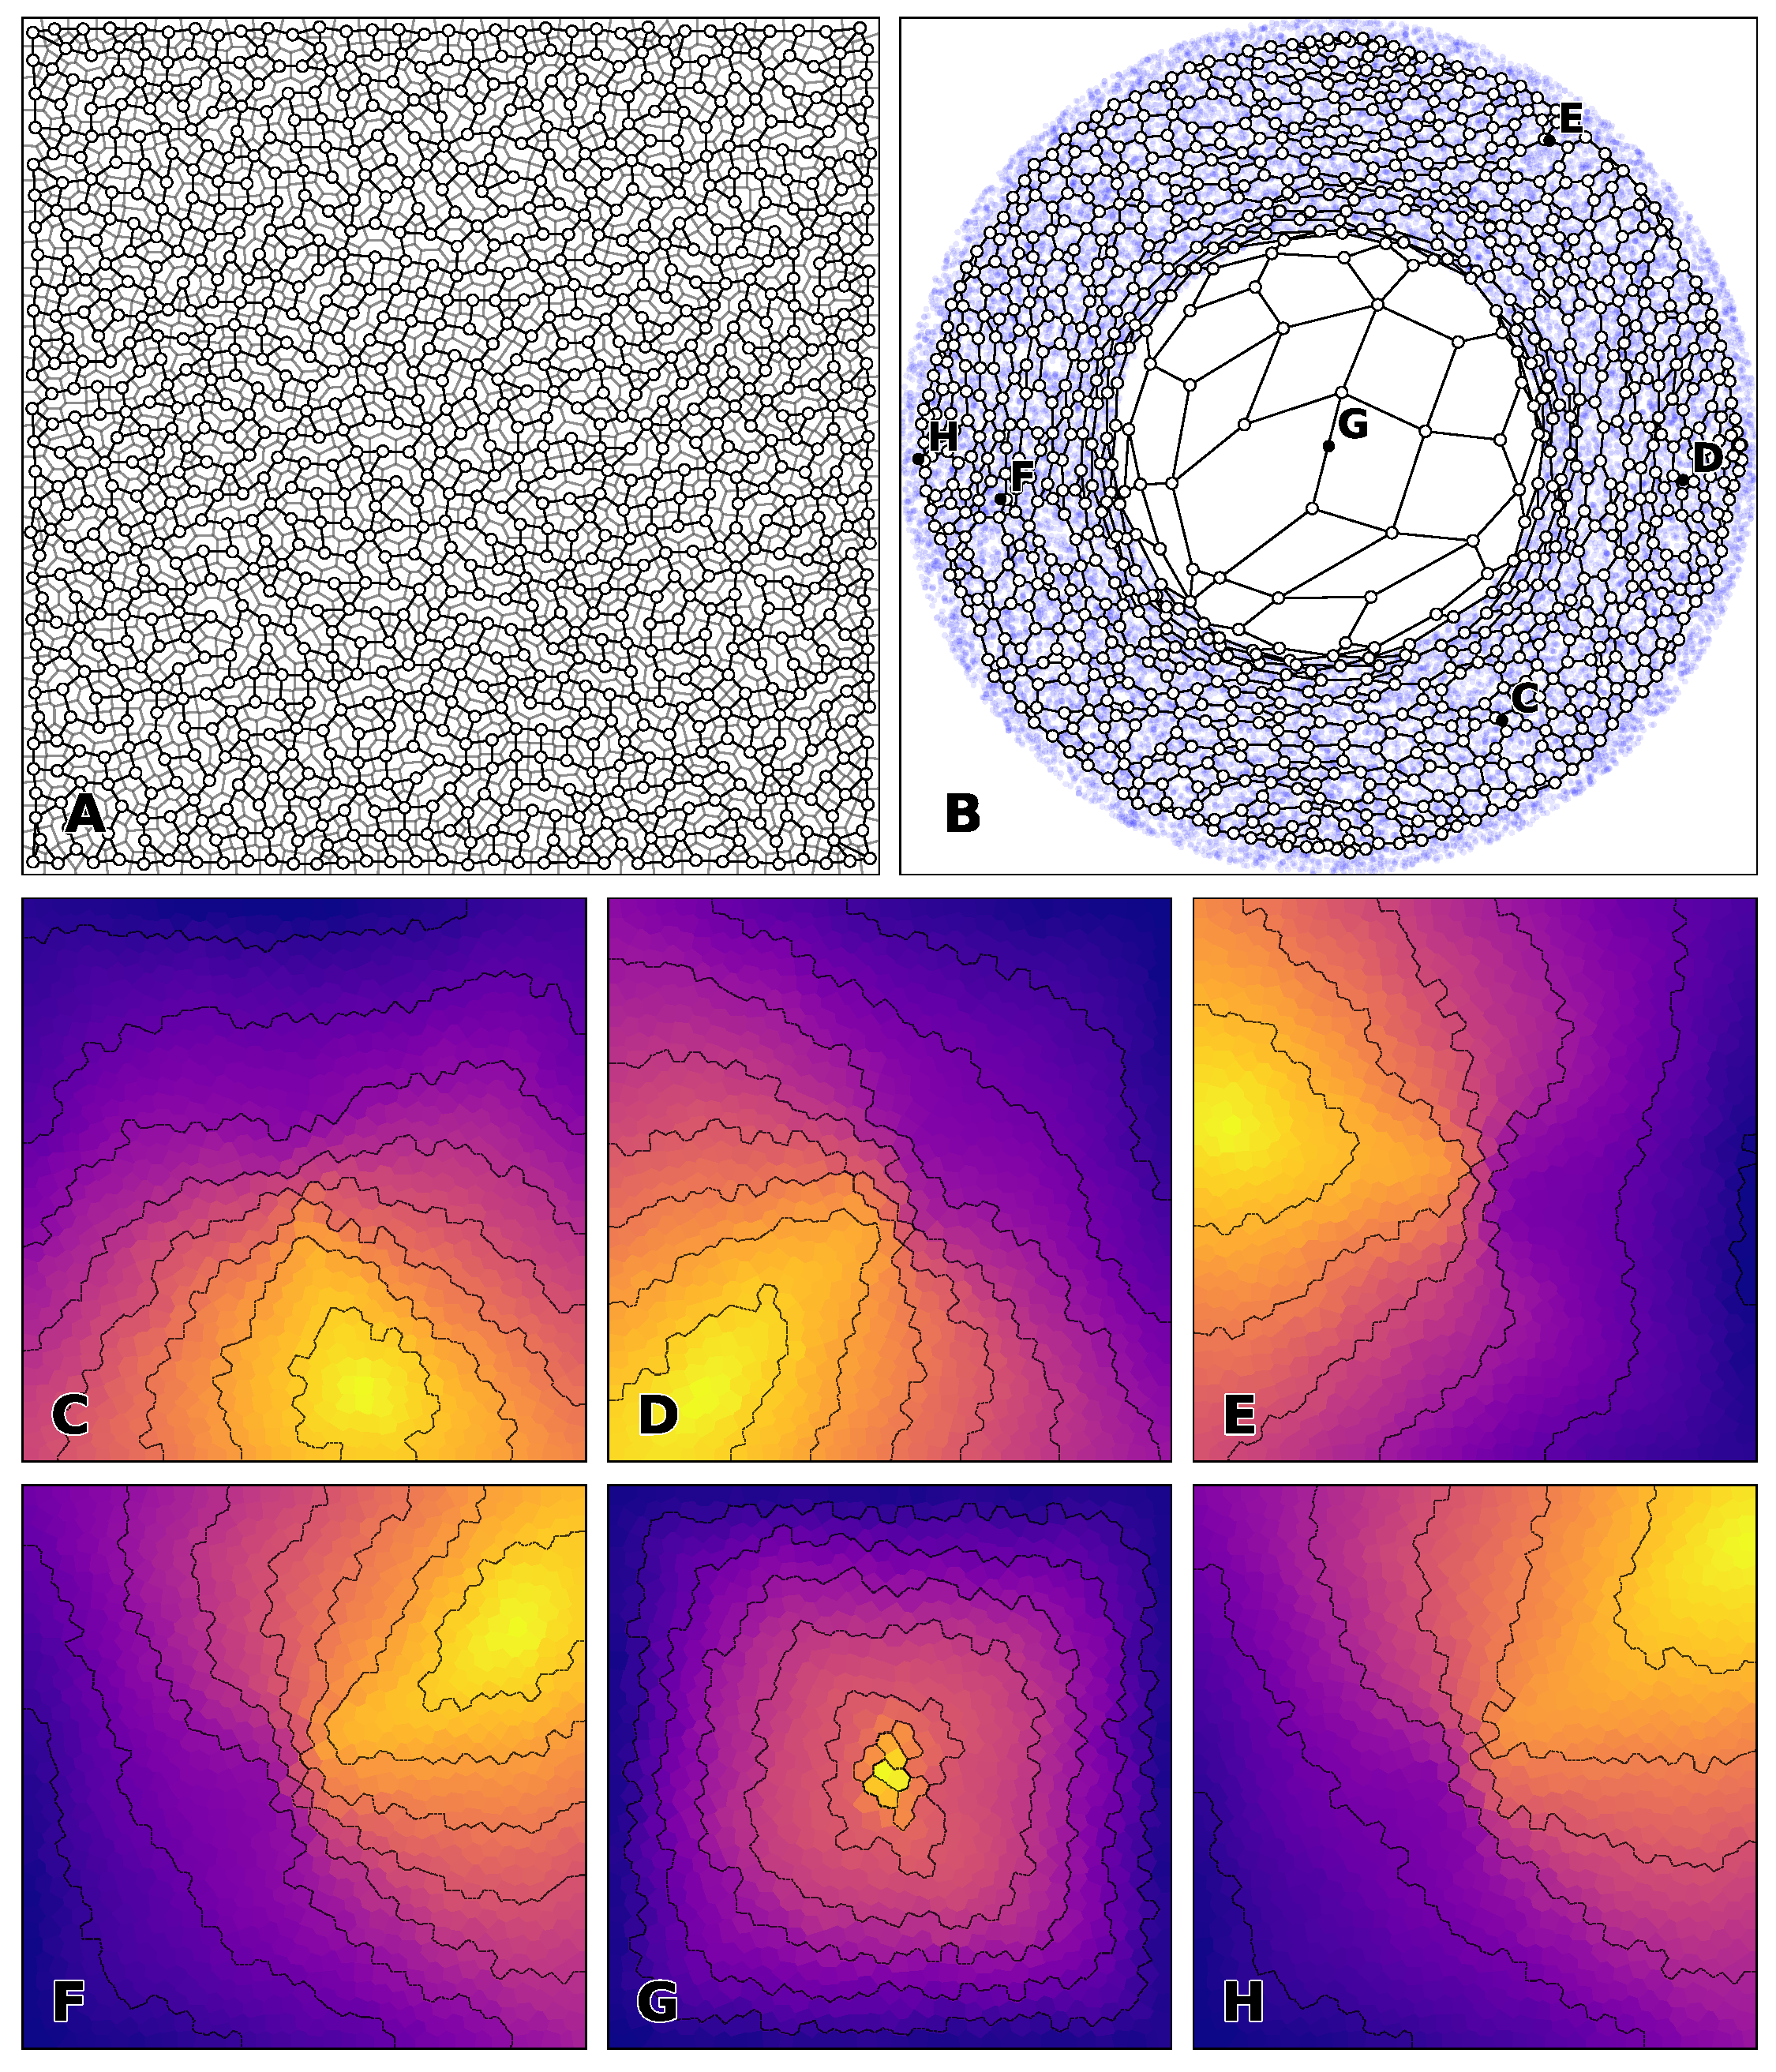
\includegraphics[width=\columnwidth]{experiment-2D-torus.pdf}
  \vspace{2mm}
  \centering
  \includegraphics[width=.975\columnwidth]{figures/colormap.pdf}
  %
  \caption{%
  %
  {\bfseries \sffamily Two dimensional ring dataset (results)}
  %
  Randomized SOM made of $1024$ neurons with a $3$-nearest neighbors induced topology. Model has been trained for $25,000$ epochs on two-dimensional points drawn from a ring distribution on the unit square. \textbf{A} Map topology in neural space. \textbf{B} Map topology in data space. \textbf{C to H} Normalized distance map for six samples. Normalization has been performed for each sample in order to enhance contrast but this prevents comparison between maps.
  %
  }
  \label{fig:2D-ring:results}
\end{figure}


% A one-dimensional problem as the one in the previous paragraph does not reveal a lot of information with respec to the organization of the map. Therefore, we proceed with investigating how a two-dimensional map learns two-dimensional representations. First, we train the SOM algorithms (both the Kohonen and VSOM) on $25000$ two-dimensional points drawn from a uniform distribution of an annulus in $[0, 1]\times[0, 1$]. More precisely, $x_1 = \frac{1 + r \cos(k)}{2}$ and $x_2 = \frac{1 + r\sin(k)}{2}$, where $k \sim \mathcal{U}(0, 2\pi)$ and $r \sim \sqrt{\mathcal{U}(\frac{1}{4}, 1)}$. After placing the neurons on the appropriate positions on neural space with respect to the topology provided by a blue noise distribution (only for the VSOM algorithm), we train the maps for $25000$ epochs. Both Kohonen and VSOM algorithms use $1024$ neurons. The results after convergence are shown in Figure~\ref{fig:annulus}, where the map topology of the annulus is shown in Figure~\ref{fig:annulus}{\bfseries \sffamily A}. The mapping produced by the VSOM learning algorithm is shown in Figure~\ref{fig:annulus}{\bfseries \sffamily B} trained on the annulus data set. As we observe the map covers the input space with higher density within the annulus, where the input data points lie, and a lower density within the hole of annulus. Panels~\ref{fig:annulus}{\bfseries \sffamily C}-{\bfseries \sffamily H} display the responses of six neurons (see the red annotated points in panel~\ref{fig:annulus}{\bfseries \sffamily B}) to a stimulus derived from  the discretization of $[0, 1]\times [0, 1]$. The responses of these neurons are well organized and reflect their receptive fields. 

% The distribution of eigenvalues for the two maps (black and blue colors correspond to VSOM and Kohonen maps, respectively) for the current experiment are shown in Figure~\ref{Fig:distributions}{\bfseries \sffamily A}. We observe that there is no significant difference between the two distributions and thus the two algorithms perform equally (see Section~\ref{sec:gram} for more details about how we obtain the distributions). Also the Wasserstein distance indicates that the two distributions are almost identical. 

% Finally, the persistence barcodes and diagrams in Figure~\ref{Fig:persistence_exp2} indicate that the Kohonen map (middle column in the figure) does not capture so well the $H1$ topological features of the input (first column in the figure),  although it captures the $H1$ properties. This is related to the fact that the  Kohonen map covers with more neurons the hole of the annulus which is not  the case with the VSOM. VSOM retains better than Kohonen the $H1$ topological features and this is reflected in the barcode and diagram (last column) where the blue dots resemble the cluster of blue dots of input's diagram (first column). This indicates that VSOM uses less neurons to cover the hole of the annulus, which can be confirmed by visually inspecting Figure~\ref{fig:annulus}{\bfseries \sffamily B}. The same phenomenon is present in the persistent barcodes where the blue segments appear in input's and VSOM's barcodes but not as strongly as in Kohonen's. 

\subsection{Oriented Gaussians dataset}


\begin{figure}
  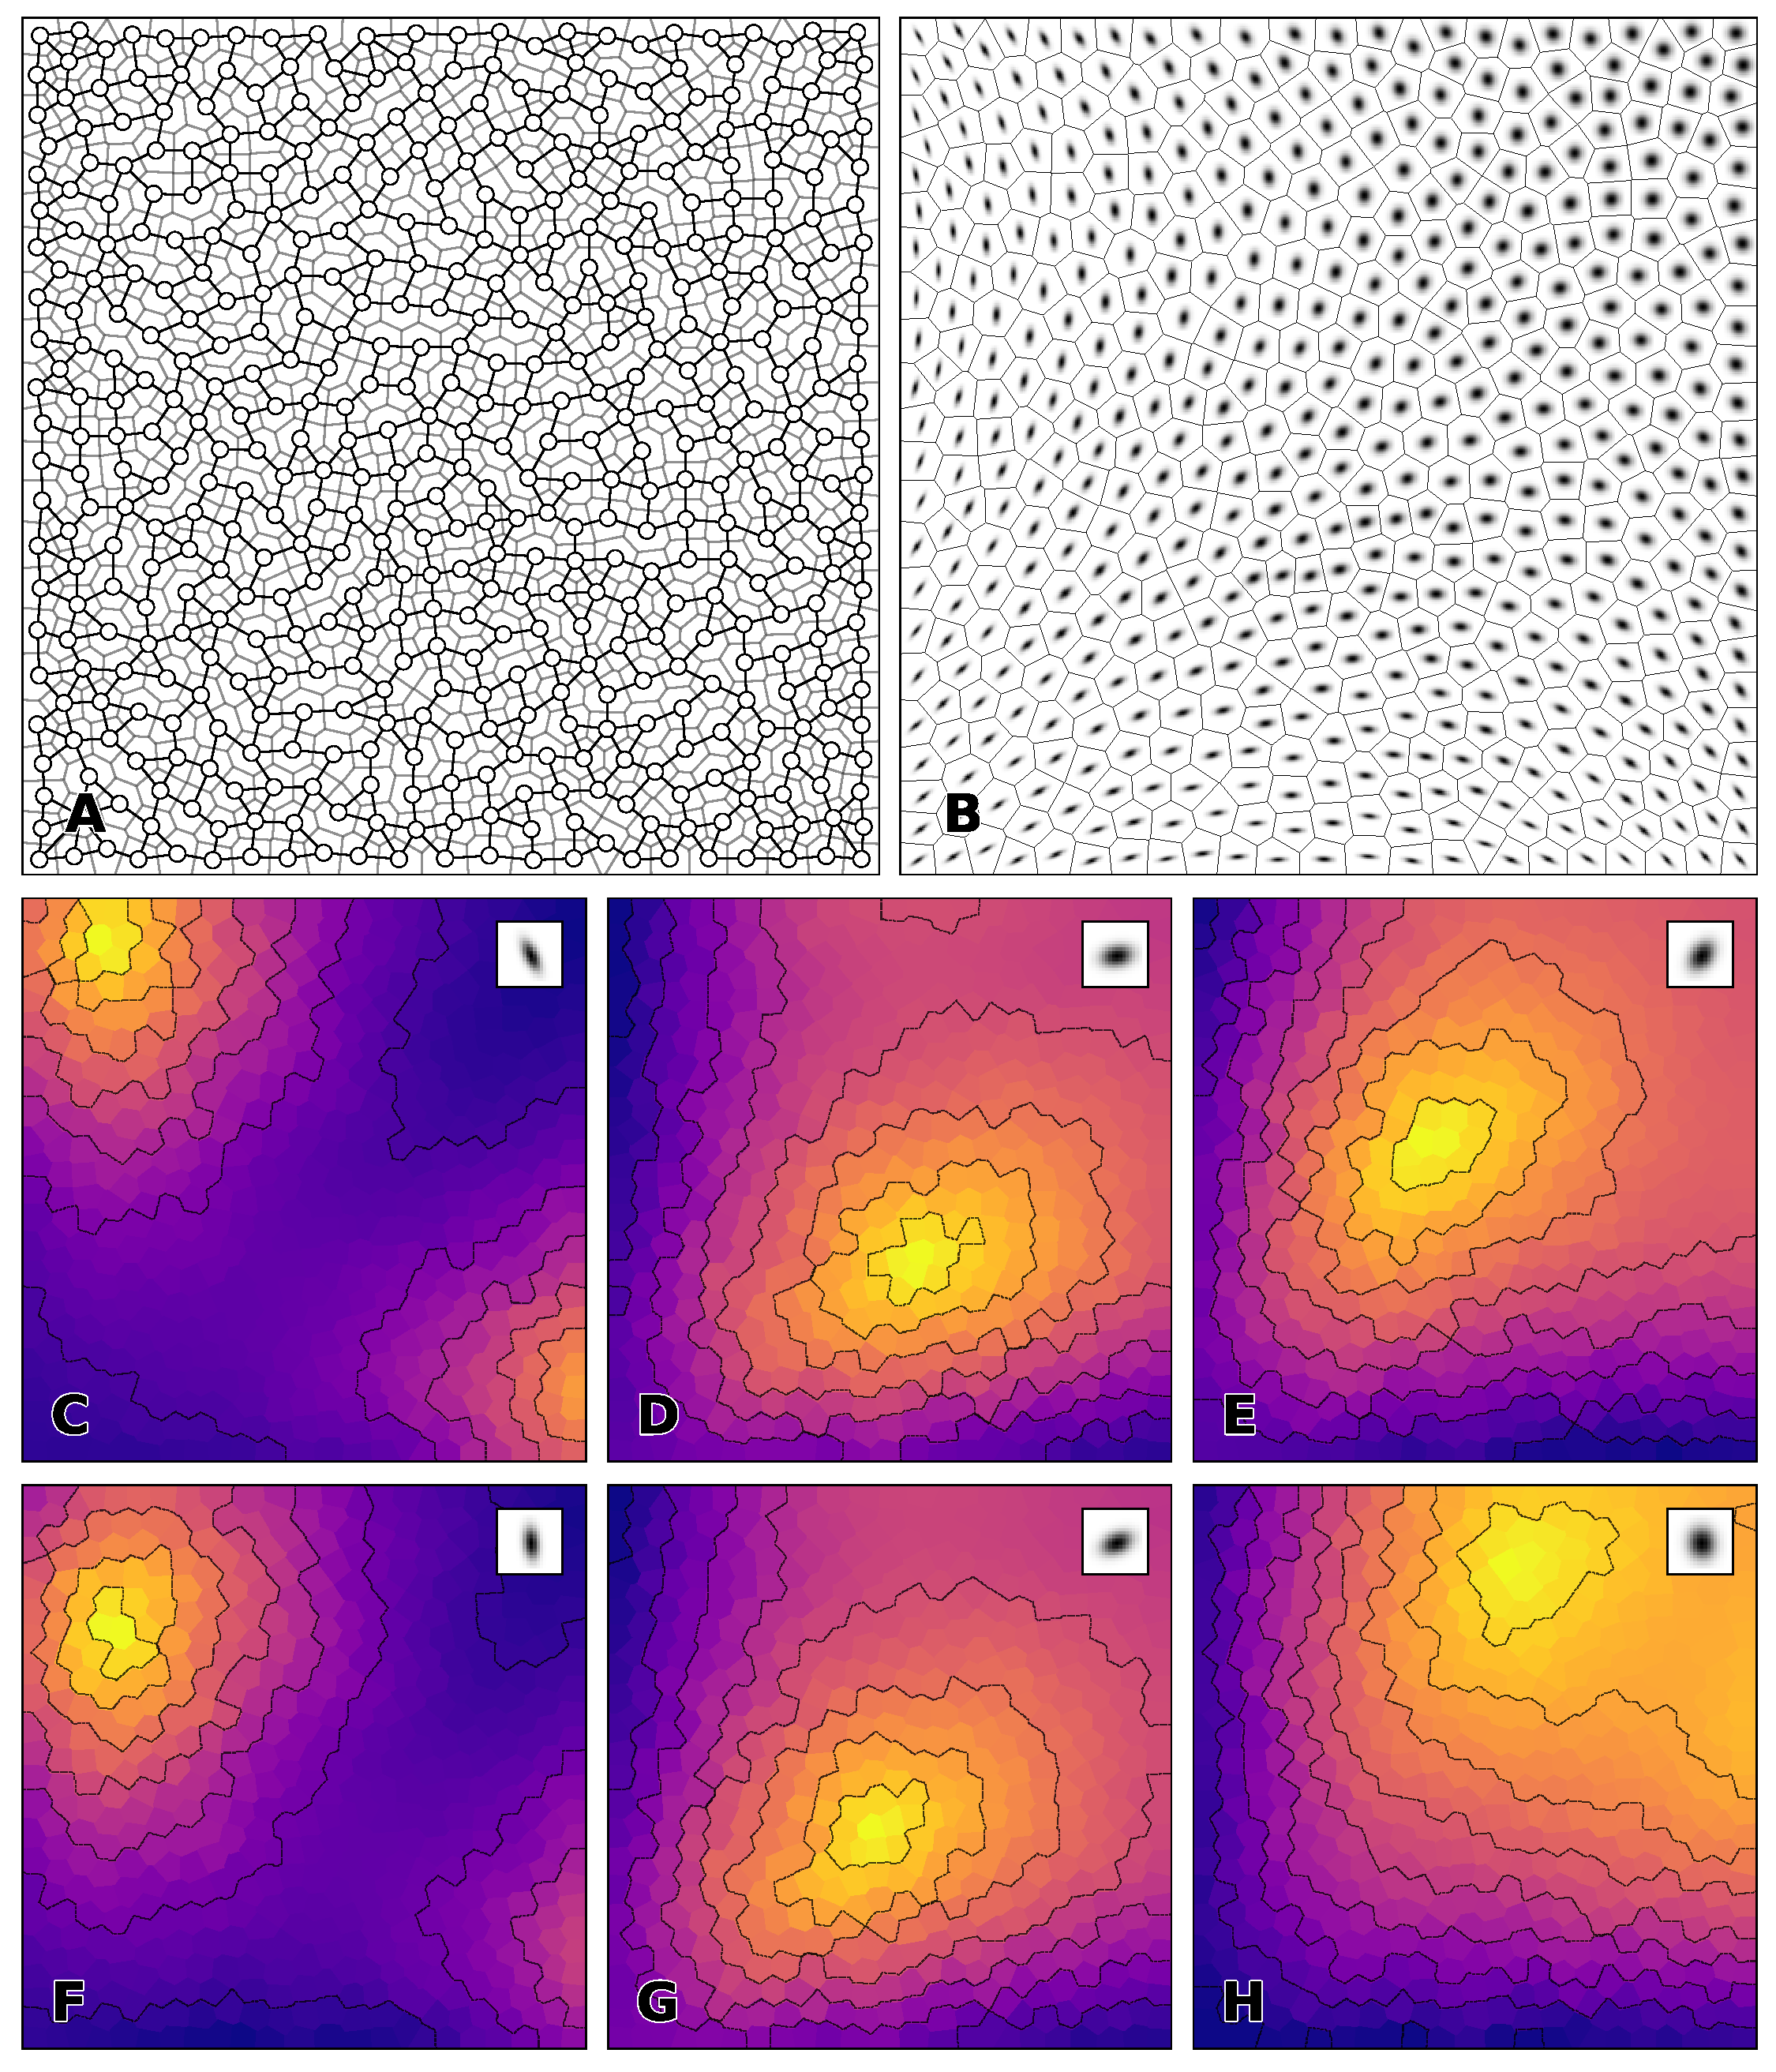
\includegraphics[width=\columnwidth]{experiment-Gaussians.pdf}
  \vspace{2mm}
  \includegraphics[width=\columnwidth]{colormap.pdf}
  %
  \caption{%
  %
  {\bfseries \sffamily Oriented Gaussians dataset (results)}
  %
  Randomized SOM made of $1024$ neurons with a $2$-nearest neighbors induced topology. Model has been trained for $25,000$ epochs on oriented Gaussian datasets. \textbf{A} Map topology in neural space. \textbf{B} Map topology in data space. \textbf{C to H} Receptive field of the map for six samples.
  %
  }
  \label{fig:gaussians:results}
\end{figure}

\subsection{Influence of the topology}

\begin{figure}
  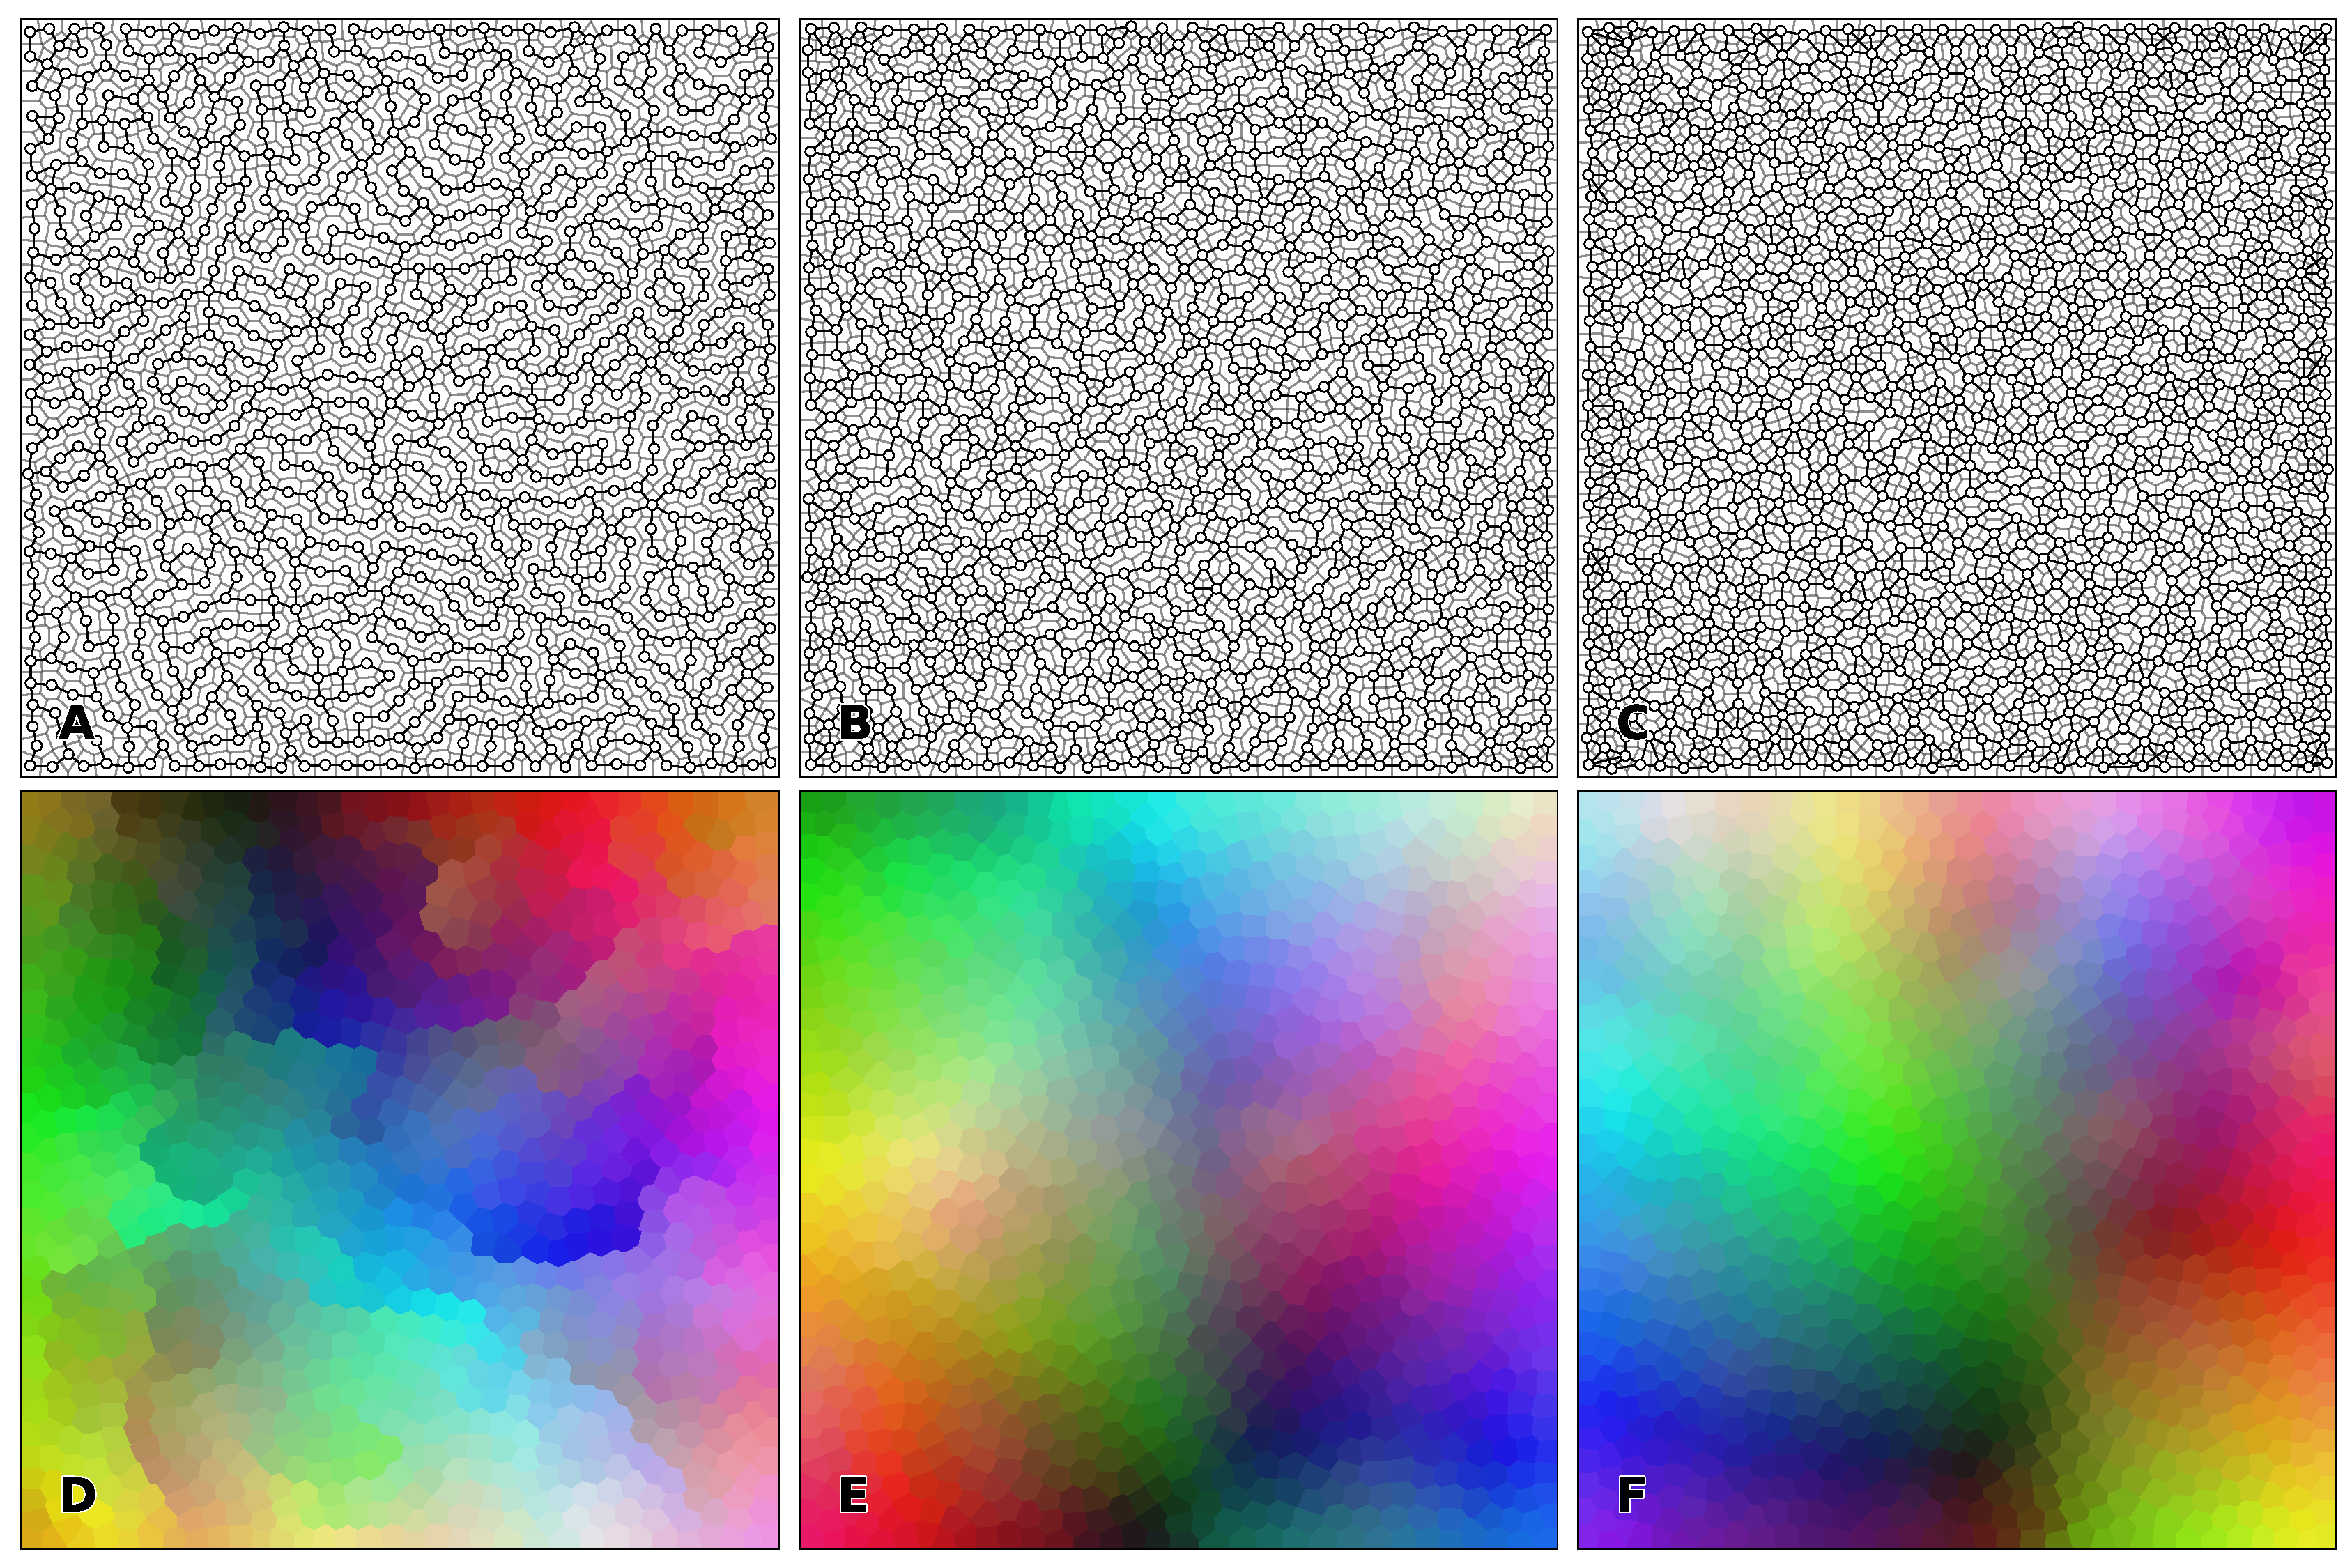
\includegraphics[width=\columnwidth]{figure-topology-influence.pdf}
  %
  \caption{%
  %
  \textbf{Influence of topology on the self organization.}
  %
  The same initial set of 1024 neurons has been equiped with 2-nearest neighbors, 3 nearest neighbors and 4-nearest neighbors induced topology (panels \textbf{A}, \textbf{B} and \textbf{C} respectively) and trained on 25,000 random RGB colors. This lead to qualitatively different self-organization as shown on panels \textbf{D}, \textbf{E} and \textbf{F} respectively, with major discontinuities in the 2-nearest neighbors case. ).
  %
  }
  %
  \label{fig:topology-influence}

\end{figure}

\subsection{Eigenvalues distribution}
\label{sec:dist}

One way to investigate if there is any significant difference between the regular and random SOMs is to compare their neural responses to the same random stimuli. Therefore, we measure the neural activity and build a covariance matrix out of it. Then, we compute the eigenvalues of the covariance matrix (or Gram matrix) and we estimate a probability distribution. Thus, we can compare the eigenvalues distributions of the two maps and compare them to each other. If the distributions are close enough in the sense of Wasserstein distance then the two SOMs are similar in terms of neural activation.  A Gram matrix is an $n \times n$ matrix given by where $n$ is the number of neurons of the map and ${\bf Y} \in \mathbb{R}^{n \times m}$ is a matrix for which each column is the activation of all $n$ neurons to a random stimulus.

From a computational point of view we construct the matrix ${\bf Y}$ by applying a set of stimuli to the self-organized map and computing the activity of each neuron within the map. This implies that ${\bf Y} \in \mathbb{R}^{m \times n}$, where $m=1024$ (the number of neurons) and $n={2, 3}$ (two- or three-dimensional input samples). Then we compute the covariance or Gram matrix as ${\bf M} = {\bf Y}{\bf Y}^T \in \mathbb{R}^{n \times n}$, where $n$ is the number of neurons. Then we compute the eigenvalues and obtain their distribution by sampling the activity of neurons of each experiment for $200$ different initial conditions using $50$ input sample each time. At the end of sampling we get an \emph{ensemble} of $200$ Gram matrices and finally we estimate the probability density of the eigenvalues on each \emph{ensemble} by applying a Kernel Density Estimation method~\citep{Parzen:1962} (KDE) with a Gaussian kernel and bandwidth $h=0.4$. This allows us to quantify any differences on the distributions of the regular and randomized SOMs by calculating the Earth-Mover or Wasserstein-1 distance over the two distributions (regular ($P$) and random SOM ($Q$)). The Wasserstein distance is computed as $W(P, Q) = \inf_{\gamma \in \Pi(P, Q)}\{\mathbb{E}_{(x, y) \sim \gamma}\Big[||x - y||\Big]\}$, where $\Pi(P, Q)$ denotes the set of all joint distributions $\gamma (x, y)$, whose marginals are $P$ and $Q$, respectively. Intuitively, $\gamma (x,y)$ indicates  how  much ``mass'' must be transported from $x$ to $y$ to transform the distribution $P$ into the distribution $Q$. 

The distributions of the eigenvalues of the RSOM and the regular SOM are shown on figure~\ref{fig:eigenvalues}. We can conclude that the two distributions are alike and do not suggest any significant difference between the two maps in terms of neural activity. This implies that the RSOM and the regular SOM have similar statistics of their neural activities. This means that the loss of information and the \emph{stretch} to the input data from both RSOM and regular SOM are pretty close and the underlying  topology of the two maps do not really affect the neural activity. This is also confirmed
by measuring the Wasserstein distance between the two distributions. The blue curve shows the regular SOM or distribution $P$ and the black curve the RSOM or distribution $Q$. The Wasserstein distance between the two distributions $P$ and $Q$ indicates that the two distributions are nearly identical on all datasets. The Wasserstein distances in Table~\ref{table:distances}
confirm that the eigenvalues distributions of SOM and RSOM are almost identical indicating that both maps retain the
same amount of information after learning the representations of input spaces.

\begin{table}[!ht]
  \begin{center}
    \begin{tabular}{ll}
        \textbf{Experiment} & \textbf{Wasserstein Distance} \\
        \hline
        $2$D ring dataset               & $0.0000323$\\
        $2$D uniform dataset with holes & $0.0000207$  \\
        $3$D uniform dataset            & $0.0001583$ \\
        MNIST dataset                   & $0.0015$ \\
    \end{tabular}
      \caption{\textbf{Wasserstein distances of eigenvalues distributions.} We report here the Wasserstein 
      distances between eigenvalues distributions of SOM and RSOM for each of the four major experiments we
      ran. The results indicate that the distributions are close pointing out that the SOM and RSOM capture
      a similar level of information during training. For more information regarding how we computed the 
      eigenvalues distributions and the Wasserstein distance please see Section~\ref{sec:dist}.}
      \label{table:distances}
  \end{center}
\end{table}

\begin{figure}
  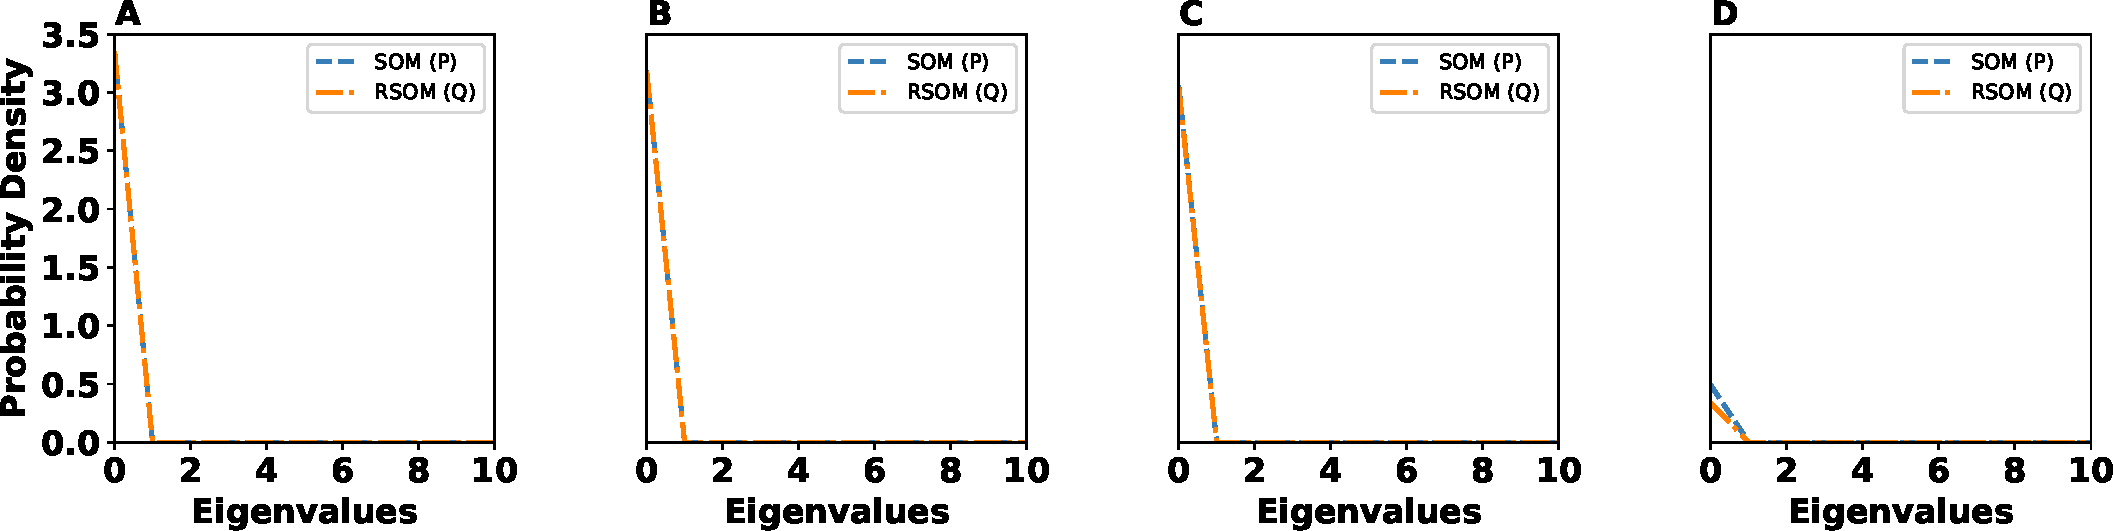
\includegraphics[width=\columnwidth]{eig-distributions-new.pdf}
  %
  \caption{Eigenvalues distribution for \textbf{A} 2D Ring dataset \textbf{B} 2D uniform dataset with holes \textbf{C} 3D uniform dataset and \textbf{D} MNIST Dataset
  }%
  \label{fig:eigenvalues}
 \end{figure}
\subsection{Distortion and entropy measures}

\begin{figure}
  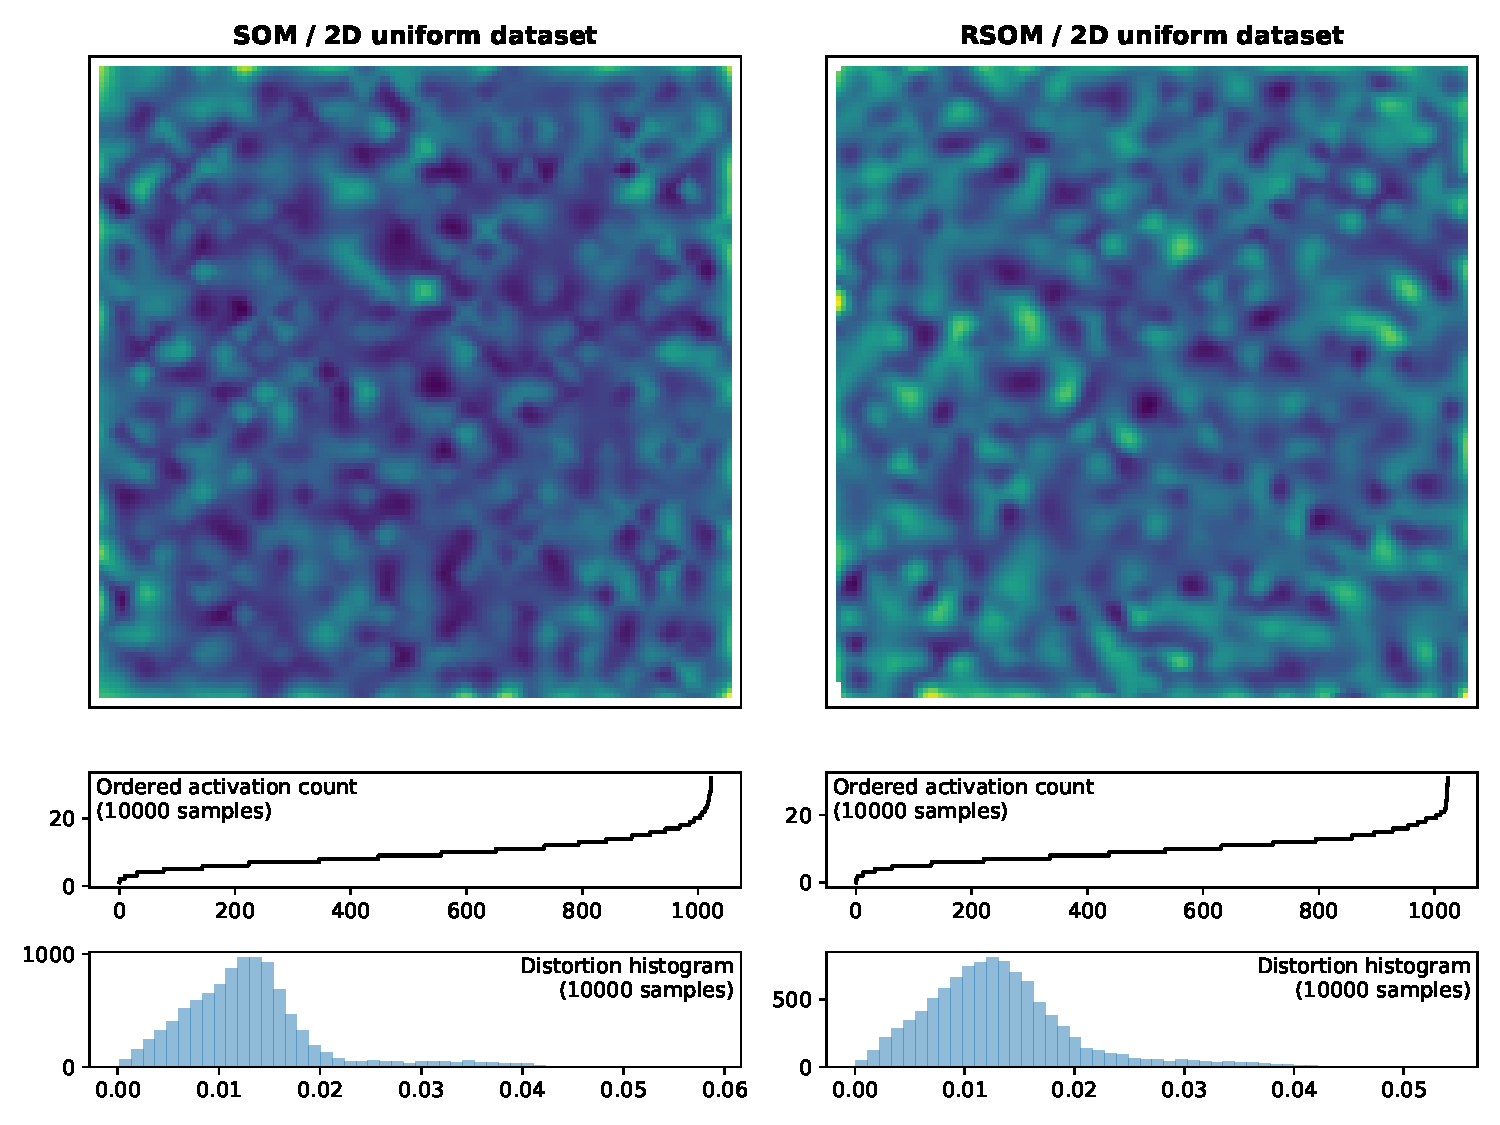
\includegraphics[width=\columnwidth]{experiment-2D-uniform-activation-distortion.pdf}
  \caption{\textbf{Two dimensional uniform dataset (measures)}. Measure of distortion and mean activation over 10,000 samples.}%
\end{figure}

\begin{figure}
  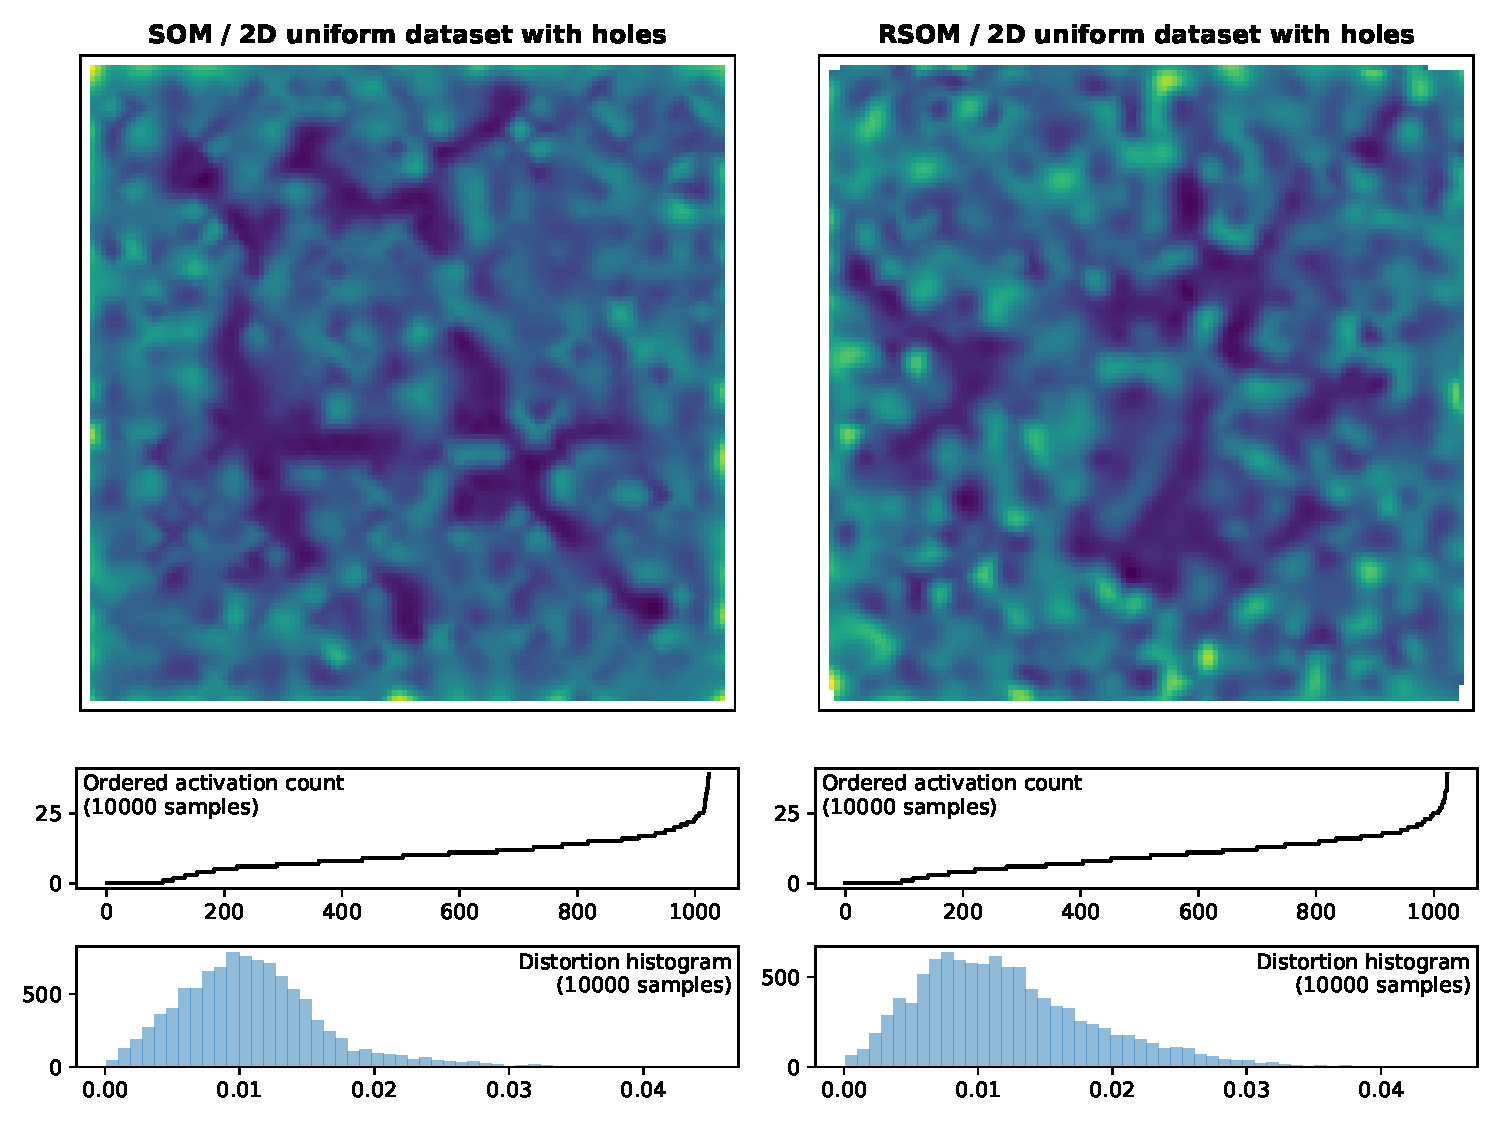
\includegraphics[width=\columnwidth]{experiment-2D-holes-activation-distortion.pdf}
  \caption{\textbf{Two dimensional uniform dataset with holes (measures)}Measure of distortion and mean activation over 10,000 samples.}%
\end{figure}

\begin{figure}
  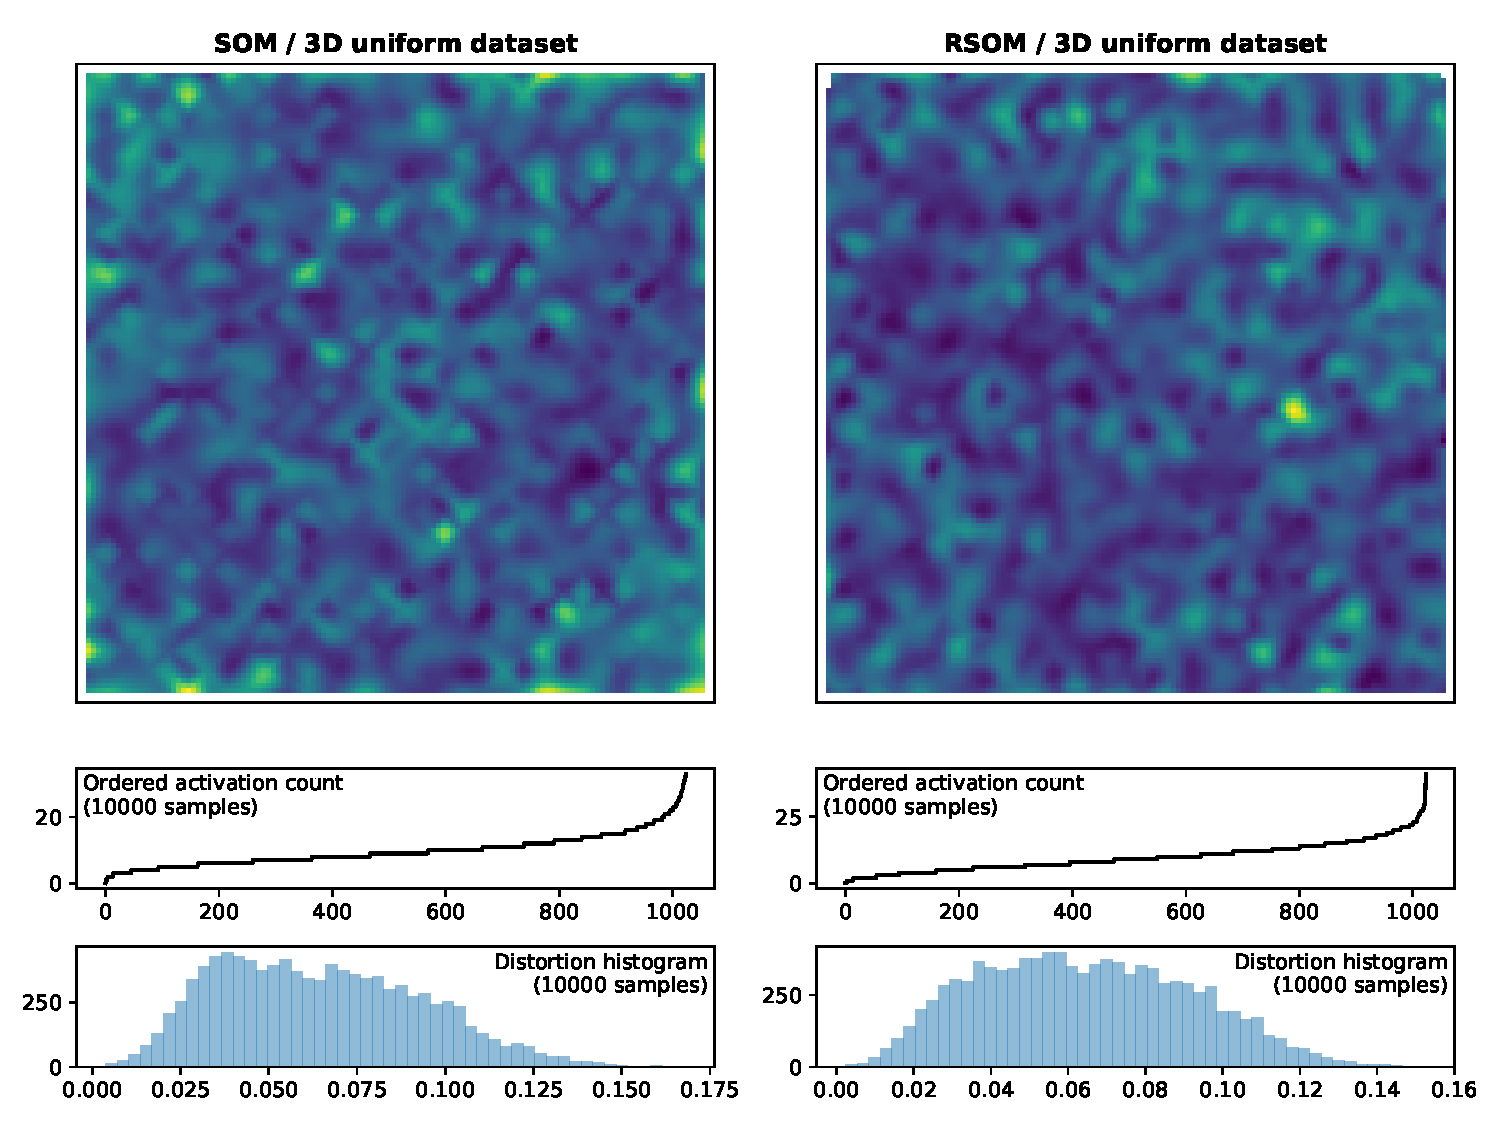
\includegraphics[width=\columnwidth]{experiment-3D-uniform-activation-distortion.pdf}
  \caption{\textbf{Three dimensional uniform dataset (measures)}. Measure of distortion and mean activation over 10,000 samples.}%
\end{figure}

\begin{figure}
  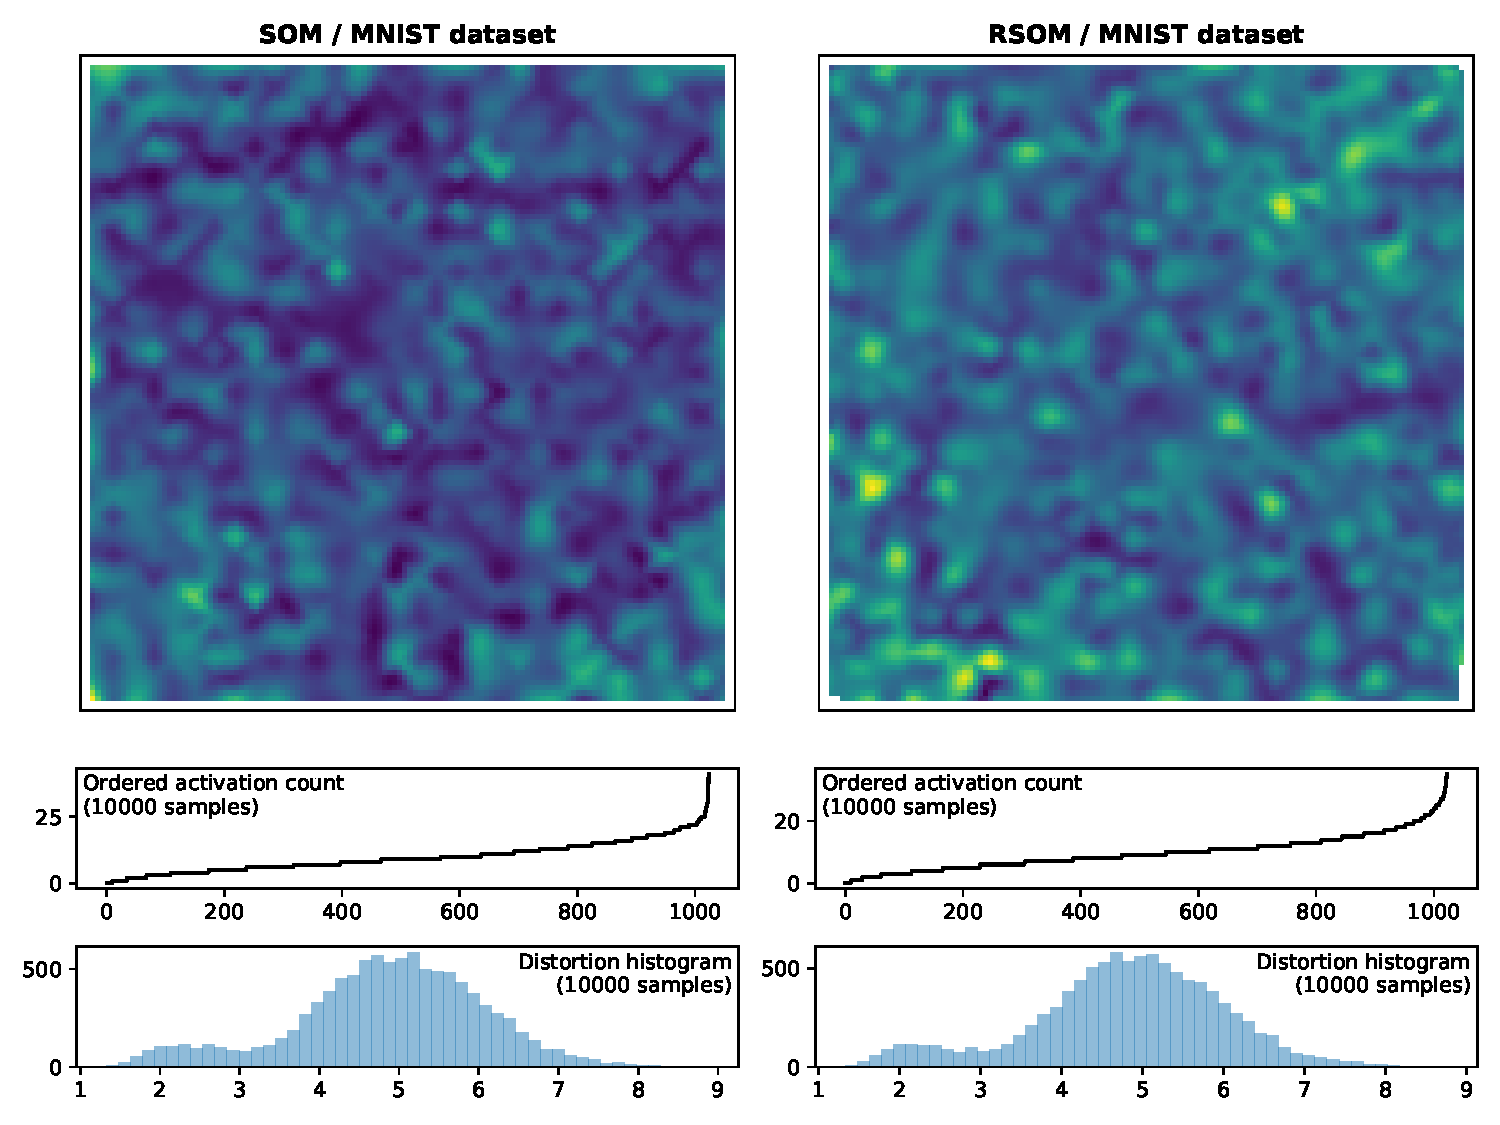
\includegraphics[width=\columnwidth]{experiment-MNIST-activation-distortion.pdf}
  \caption{\textbf{MNIST dataset (measures)}. Measure of distortion and mean activation over 10,000 samples.}%
\end{figure}



\end{document}
